\documentclass[12pt]{report}
\usepackage[utf8]{inputenc}
\usepackage{graphicx,listings,verbatim,csquotes,amsmath,tabularx,tabulary}
\usepackage[backend=bibtex]{biblatex}
\usepackage[margin=1in]{geometry}
\addbibresource{Thesis.bib}

\begin{document}

\title{
	{Algorithms and Applications of the Vision Correcting Display}\\
	{\large University of California, Berkeley}\\
}
\author{Charles Ding}
\date{12 May 2017}

\maketitle

\chapter*{Abstract}
Human vision problems such as nearsightedness and farsightedness are a result of optical aberrations in the human eye. The common method of treating eye aberrations is wearing corrective lenses, such as glasses or contact lenses, or undergoing laser eye surgery. The vision correcting display team under Professor Brian Barsky aims to develop a light field display using hardware and software that lets the user see a digital screen clearly without glasses or contact lenses. In addition, the team writes software simulations of the vision correcting display to evaluate the performance of the display for different eye aberrations and different digital devices. \\
In this paper, we present a new software approach to the display, the backward method, and compare it with the original light field algorithm \cite{Huang:EECS-2013-206} and the forward method \cite{Wu:EECS-2016-67}. We also explore two new applications of the vision correcting display: the effect of different pixel arrangements from different devices on the performance of the display and the effects of diffraction in choosing an optimal pinhole size. Finally, we present a new approach to the software simulation that combines both ray and wave optics.

\chapter*{Acknowledgements}
I want to thank my advisor Professor Brian Barsky for all his help and support during my two years as a member of his research group. Also, I want to thank all the members of the vision correcting display team, especially Michael Chen, Dingyi Zheng, Linghan Zheng, Tongyu Chen, Luxin Yang, Vivek Claver, Haonan Jing, Hung Vu, and Yirong Zhen for all their help and contributions. Finally, I want to thank Professor Laura Waller for helping me look over my thesis and teaching the computational imaging class that I took.

\tableofcontents

\chapter{Introduction}

Humans depend on their vision for every waking hour of the day. Out of the five main senses, vision is arguably the most important in acquring information about the surrounding environment. A person cannot walk in the streets, drive a car, or read if he or she cannot see. However, genetic inheritance, disease, and age will naturally lead to the loss of vision. According to the Vision Council, roughly 75 percent of all adults in the United States require some form of vision correction \cite{GlassesCrafter.com:2010:Vision}. 

The most common method for correcting eye aberrations are with glasses and contact lenses. Both seek to divert the light rays right before they reach the cornea, or front layer of the eye, so that the image displayed on the retina, or sensor of the eye, is clear. However, glasses and contact lenses may present an inconvenience. For example, a person who is far-sighted might only need his or her glasses when reading a screen close to him or her and would prefer to not always put on and take off his or her glasses. But what if instead of fixing the eye, the image is modified on the screen so that it appears clear without eyewear? Professor Brian A. Barsky has been focusing on this field for over a decade and introduces the concept of the vision correcting display in his paper \textit{An Overview of Vision Realistic Rendering and Vision Correcting Displays} \cite{SDTP:SDTP10326}:

\begin{displayquote}
The concept of a vision correcting display involves digitally modifying the content of a display using measurements of the optical aberrations of the viewer's eye so that the display can be seen in sharp focus by the user without requiring the use of eyeglasses or contact lenses. Given the measurements of the optical aberrations of a users eye, a vision correcting display will present a transformed image that when viewed by this individual will appear in sharp focus. Vision correction could be provided in some cases where spectacles are ineffective.
\end{displayquote}


\begin{figure}[ht]
  \centering
  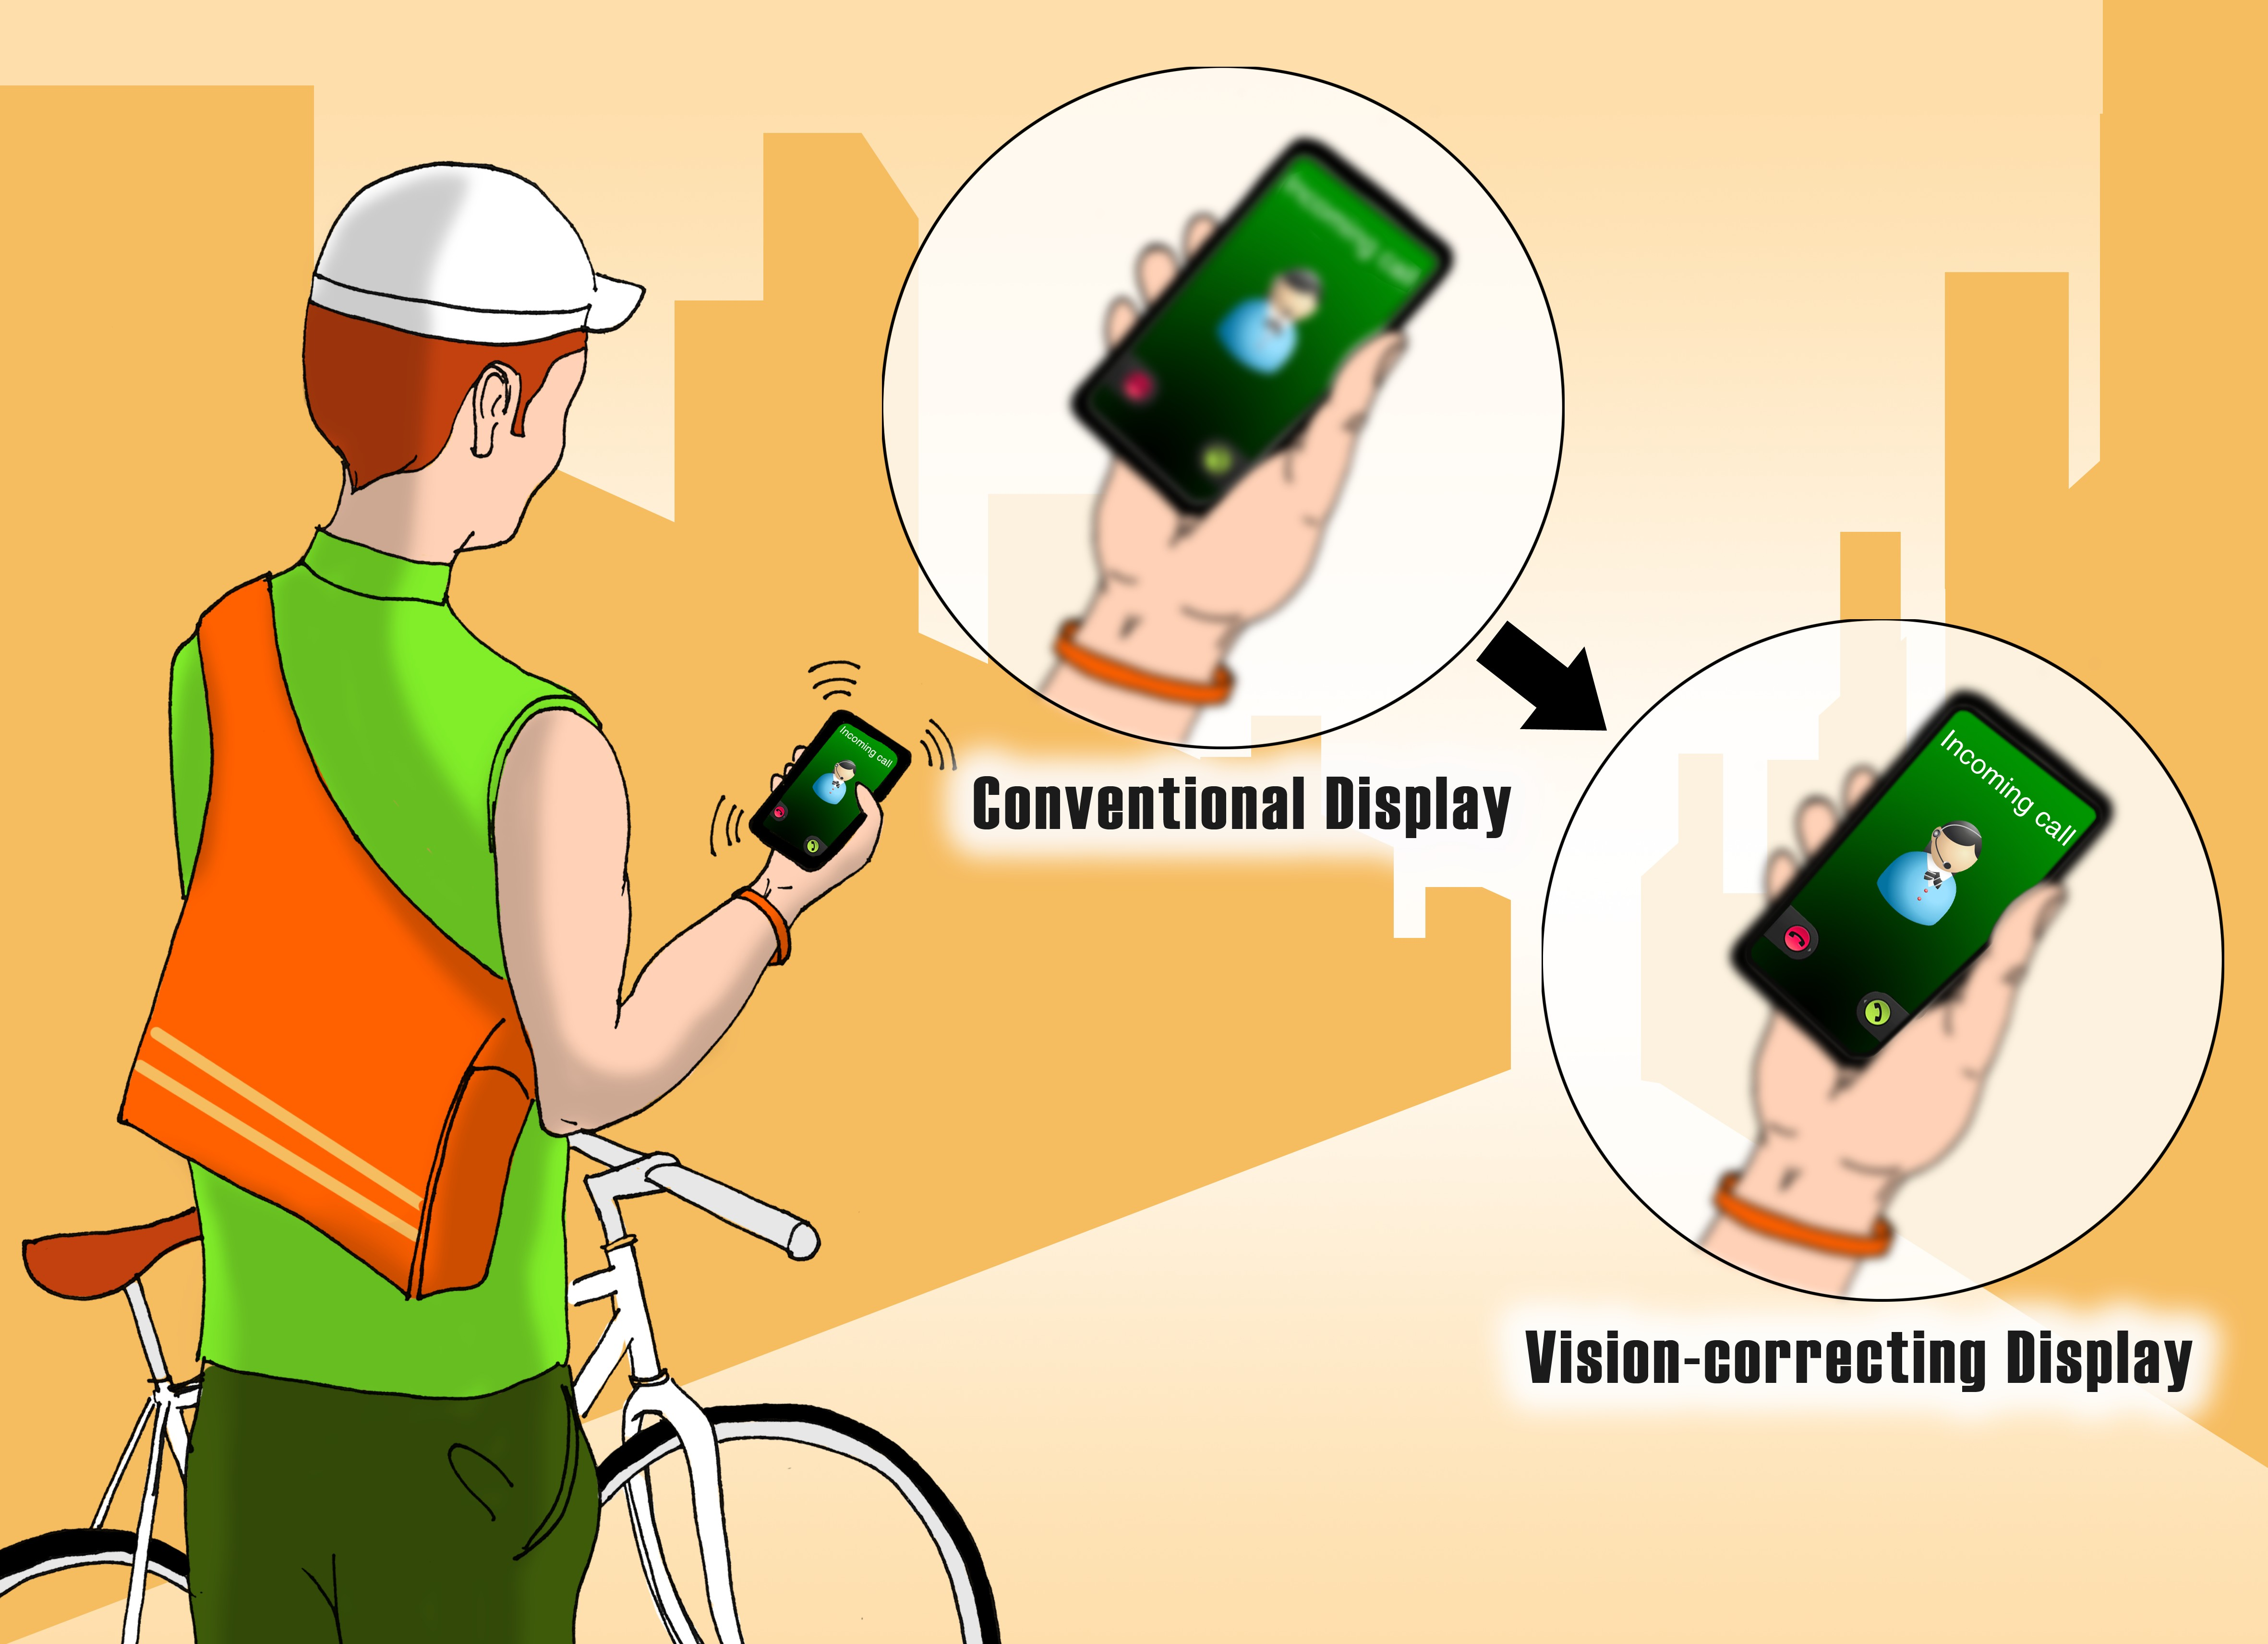
\includegraphics[height=3in]{chapters/chapter1/images/phone.jpg}
  \caption{Application Scenario of Vision-Correcting Display \cite{Huang:2014:VisionCorrectingDisplay}}
  \label{fig:application}
\end{figure}

Fu-Chung Huang et. al proposed two different solutions to this problem. In his first solution, he uses a multilayer display \cite{Huang:2012:COA:2366145.2366204}, and in the second solution, he used light field technology, specifically a pinhole mask, to generate a sharp image out of the display plane \cite{Huang:2014:VisionCorrectingDisplay}. Wu presented one new software algorithm (forward method), one major hardware improvement (lens array display), and a simulation program \cite{Wu:EECS-2016-67}. 

This paper builds on the work from Wu's report. In chapter 4, we present the backward method, which aims to fix some of the issues with the issues with Huang's algorithm. In chapter 7, we test the forward method on different RGB pixel arrangements for different phone screens. In chapter 8, we apply a combined ray and wave optics model in the simulation to account for diffraction and find the optimal size of a pinhole. Finally, in chapter 9, we compare the performance of Huang's algorithm, the forward method, and the backward method.

% TODO: Finish Reading literature on Huang's algorithm and incorporate it here

%The Chapter 2 of this paper discusses the different types of aberrations of the eye that we aim to correct. Chapters 3 and 4 describe the hardware and software components of the vision-correction display, respectively. Chapter 5 shows the performance of the vision-correction display via physical experiment. Chapter 6 describes the algorithm used for the software simulation of aberrations. Chapter 7 examines the effectiveness of the algorithms on different pixel arrangements of different devices. Chapter 8 is a case study on the effects on diffraction on the effectiveness of the display. Chapter 9 gives a summary of the results of the algorithms presented.

\chapter{Aberrations of the Eye}

We first describe the two most common forms of aberrations, myopia and hyperopia. These two types of aberrations are the easiest to illustrate via a Gaussian ray tracing model. We then go on to describe other types of aberrations such as astigmatism, coma, and trefoil, which are modeled using Zernike polynomials.  

\section{Gaussian Ray Tracing}

The Gaussian ray tracing model illustrates the path of light rays passing through a lens. The lens contains a focal point where all of the light rays are focused, and the eye focuses at a focal plane. Assume the object is located at the focal plane. In a perfect or ideal eye, the light rays traveling through the pupil converge on the sensor (retina on the eye). 

\begin{figure}[ht]
  \centering
  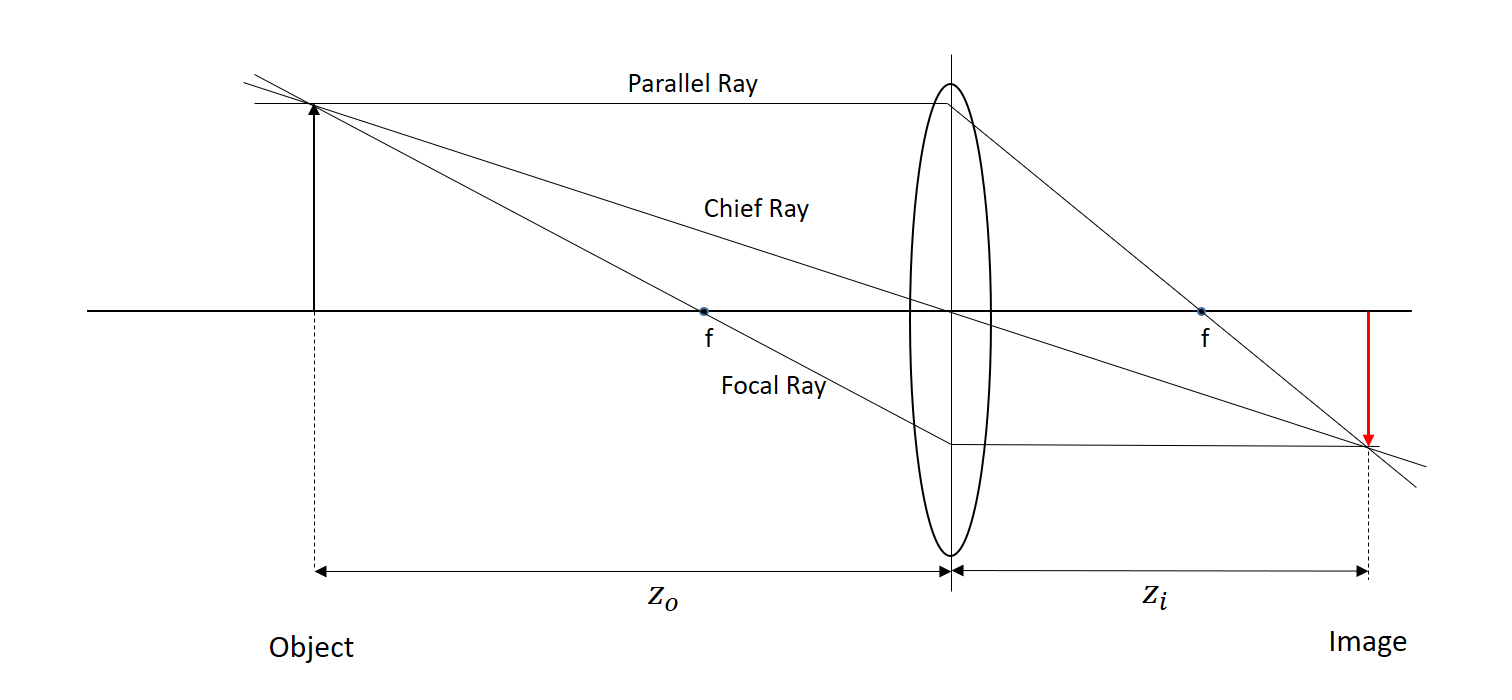
\includegraphics[width=5.0in]{chapters/chapter2/images/gauss.png}
  \caption{Gaussian Ray Tracing}
  \label{fig:ferrari}
\end{figure}

The distance from the object to the lens ($z_o$) and the distance from the image to the lens ($z_i$) are related by the following equation: 

$$\frac{1}{f} = \frac{1}{z_i} + \frac{1}{z_o}$$
 
\section{Myopia}
In a myopic or nearsighted eye, light rays converge in front of the retina. 

\begin{figure}[ht]
  \centering
  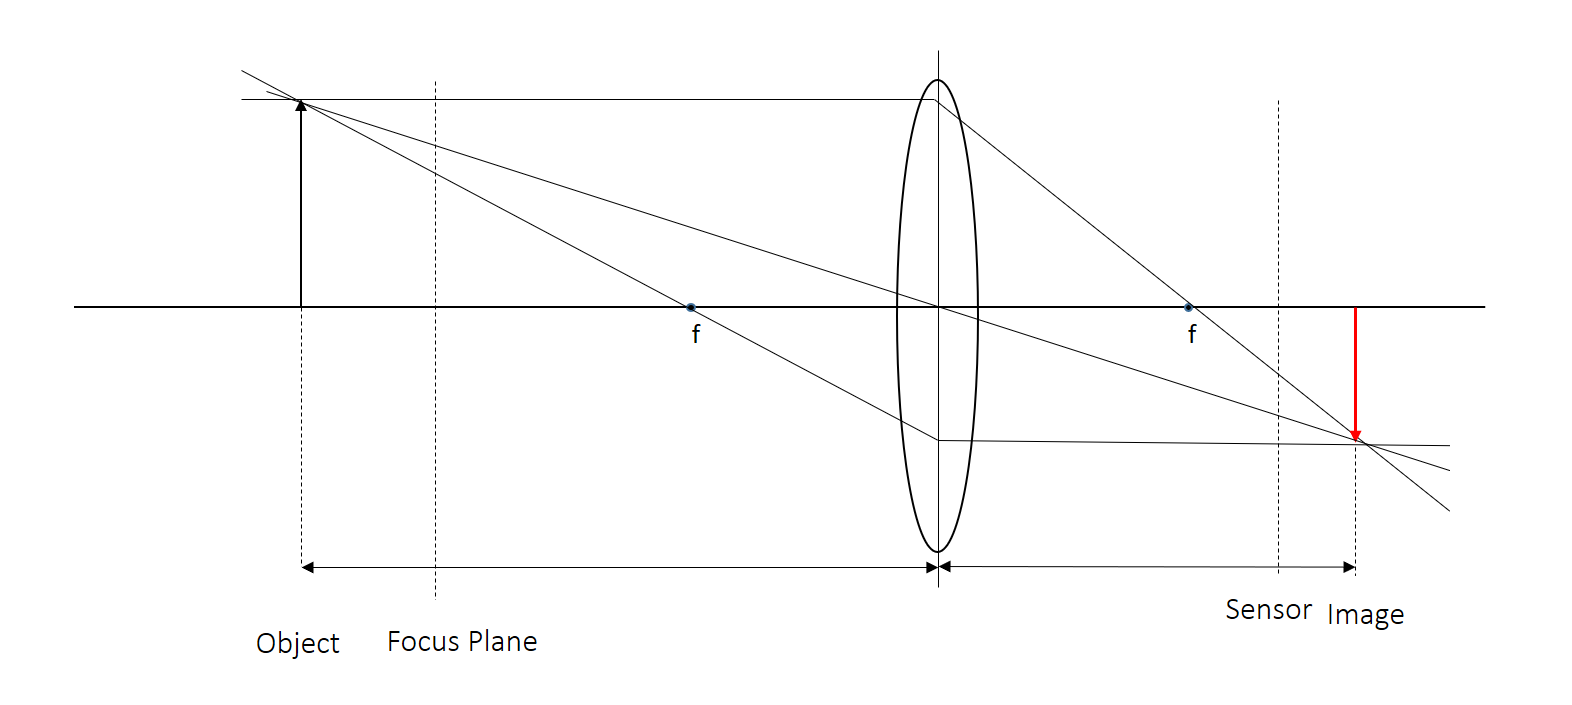
\includegraphics[width=5.0in]{chapters/chapter2/images/myopia.png}
  \caption{Myopia}
  \label{fig:ferrari}
\end{figure}

Myopia affects about 30 to 40 percent among adults in Europe and the United States, and up to 80 percent or higher in the Asian population, especially in China. In addition, incidence of myopia is increasing, from about 25 percent of Americans in the early 1970s to nearly 40 percent of the population today.

% Cite this: http://www.allaboutvision.com/parents/myopia-progression.htm

\section{Hyperopia}
In a hyperopic or farsighted eye, light rays converge behind the retina. 

\begin{figure}[ht]
  \centering
  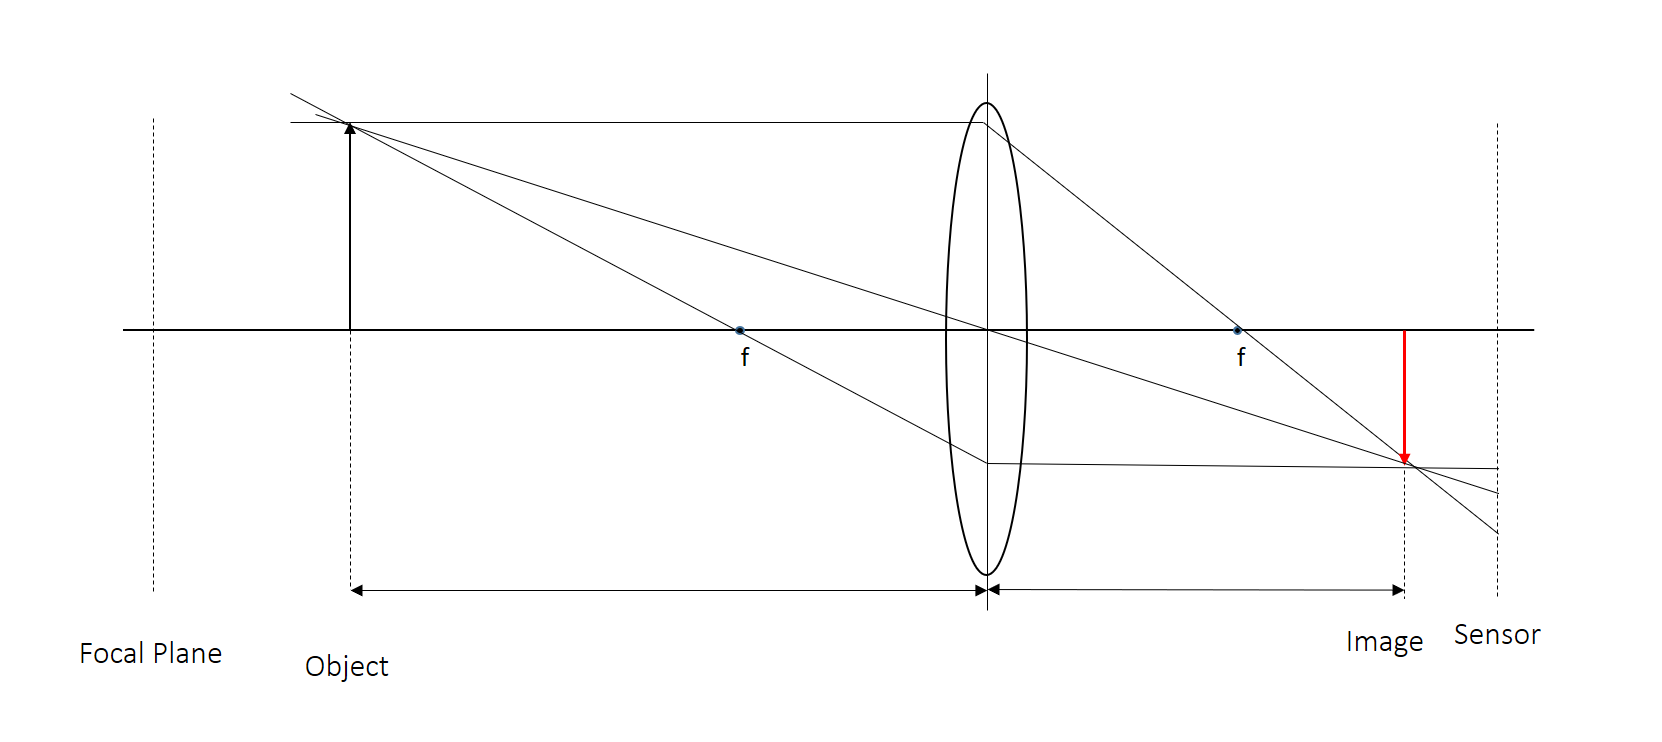
\includegraphics[width=5.0in]{chapters/chapter2/images/hyperopia.png}
  \caption{Hyperopia}
  \label{fig:ferrari}
\end{figure}

Hyperopia is a common condition that affects about ten percent of the adult population worldwide. 

% Cite this: http://www.drbishop.com/view/article_445.3conx

\section{Zernike Polynomials and Higher Order Aberrations}

We fit the wave aberrations with the Zernike polynomials, which are a set of shapes orthogonal to the unit disk used to measure the eye’s wavefront (Weisstein). The Zernike shapes are very similar to the usual aberrations that are found in a human eye. If we consider W(x,y) as the wavefront, then here is the equation that fits the Zernike polynomial:

$$W(x,y)= \sum_{i} c_i Z_i (x,y)$$

i represents the index of the coefficient c, and Z(x,y) is the associated polynomial equation. Here are the first six terms of the Zernike polynomial:

\begin{equation}
\begin{aligned}
W(x,y) ={} & c_0 \times 1 + c_1 \times 2 \times \rho \times sin(\theta) + c_2 \times 2 \times \rho \times cos(\theta) \\
           & + c_3 \times \sqrt{6} \rho^2 \times sin(2\theta) + c_4 \times \sqrt{3} \times (2 \times \rho^2 - 1) \\
           & + c_5 \times \sqrt{6} \times \rho^2 \times cos(2\theta) + ...
\end{aligned}
\end{equation}

\begin{figure}[ht]
  \centering
  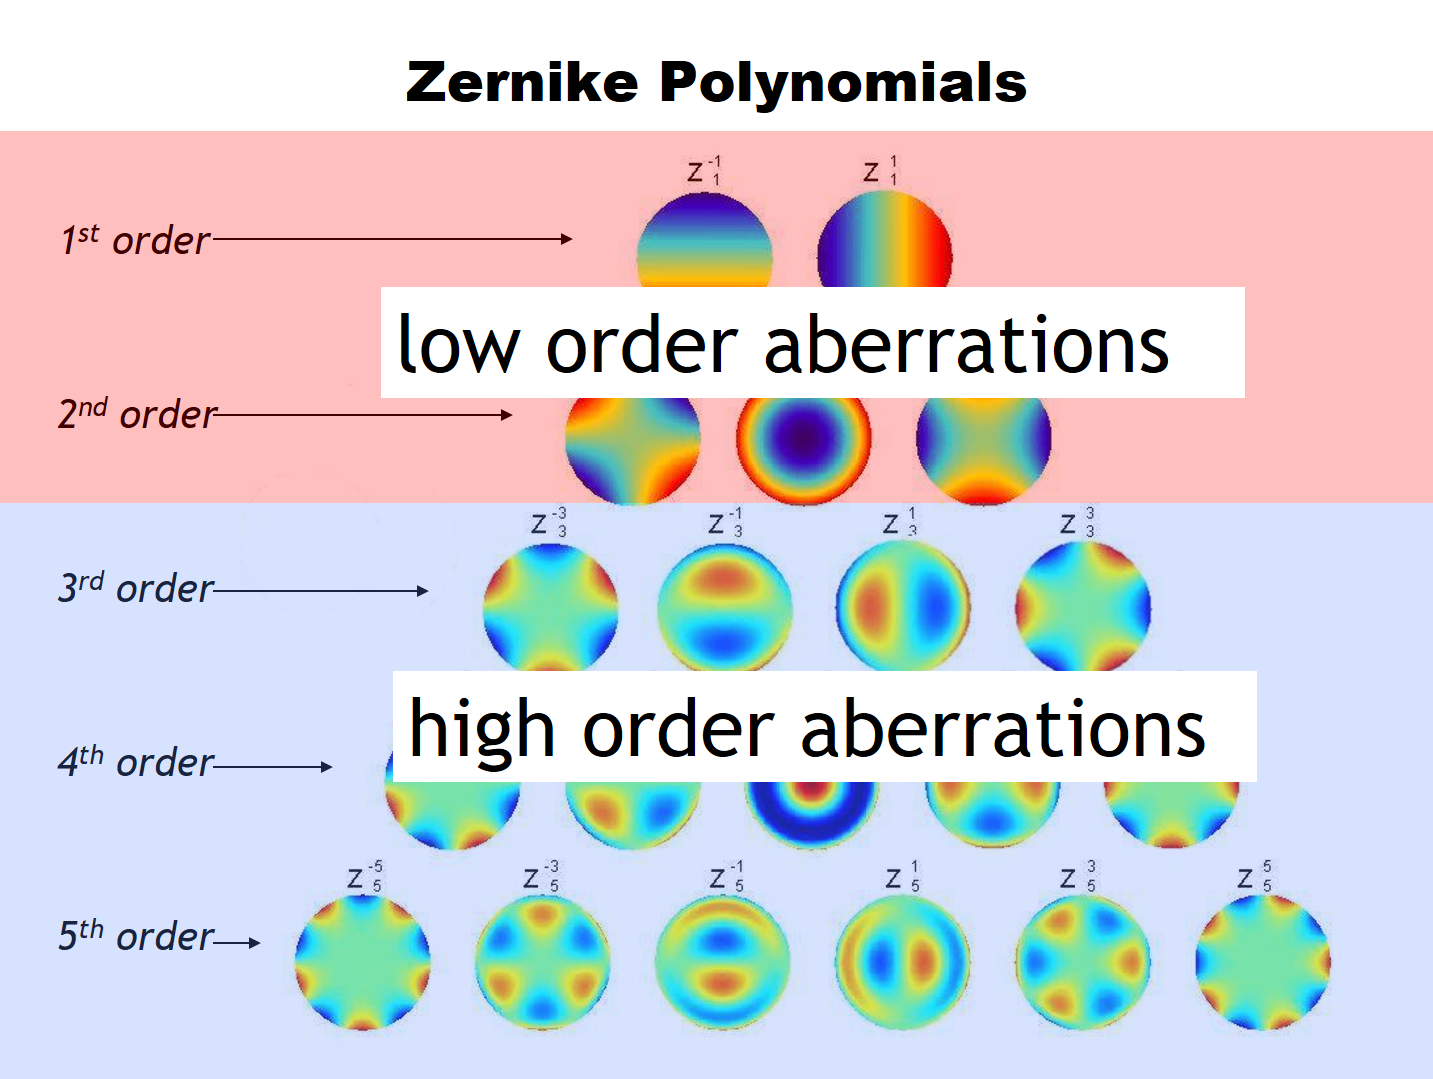
\includegraphics[width=5.0in]{chapters/chapter2/images/Zernike_polynomials.png}
  \caption{Hyperopia}
  \label{fig:ferrari}
\end{figure}

The first six Zernike polynomial terms measure lower order aberrations and the next sixty terms measure higher order aberrations. The names of lower order aberrations are tilt (terms one and two), astigmatism (terms three and five), and defocus (term four). Some examples of higher order aberrations are coma and trefoil (terms six through nine) and quatrefoil, secondary astigmatism, and spherical aberration (terms ten through fifteen). Lower order aberrations account for 90 percent of all decline in the quality of retinal images, while higher order aberrations are while the remaining 10 percent is a combination of the effects of higher order aberrations. Lower order aberrations are frequently treated with eyeglasses, which divert the direction of light rays so that they land squarely on the retina. However, higher order aberrations are much harder to treat with eyeglasses, but with the vision-correction display, a user can input the Zernike polynomial coefficients to manipulate the image on the screen.

% Cite this paper: http://www.scielo.br/pdf/rbof/v73n6/0034-7280-rbof-73-06-0358.pdf

% Question: Do I cite the PSF and wavefront map stuff?

% Do I mention circle of confusion?


% Cite Professor Austin's powerpoint slide



\chapter{Hardware of the Vision Correction Display}

We explore two hardware devices used for the vision-correction display: the pinhole mask and the lenslet array. Both devices are examples of light field displays.

\section{Light Field Display}
A light field is a vector function that describes the amount of light flowing in every direction through every point in space. The direction of each ray is given by the 5D plenoptic function $$L(x, y, z, \theta, \phi)$$, where (x, y, z) represents the position of the ray and $(\theta, \phi)$ represents the direction. The magnitude of the light ray is equivalent to its radiance, denoted by $L$ and measured in watts ($W$) per steradian ($sr$) per meter squared ($m^2$). The steradian is a measure of solid angle, or the subtended surface area on the unit sphere, and meters squared are used here to measure cross-sectional area.

\begin{figure}[ht]
  \centering
  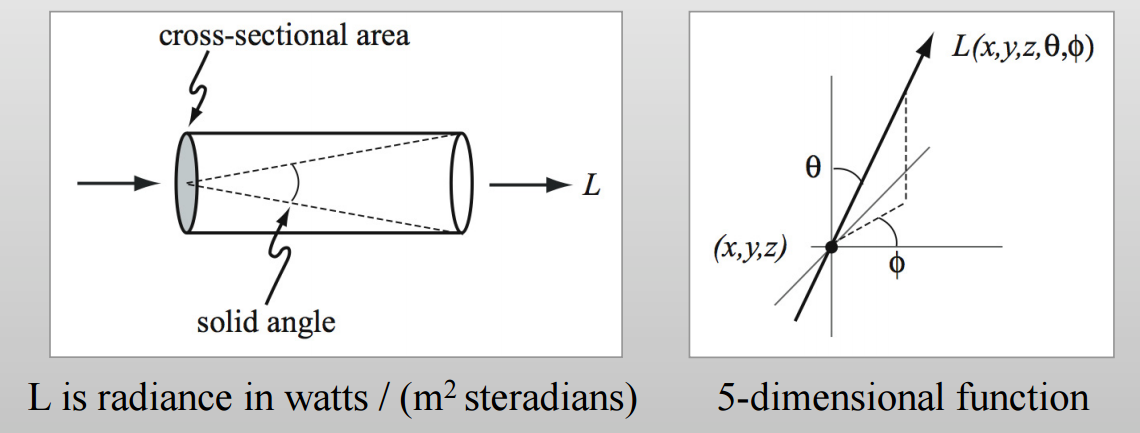
\includegraphics[width=5in]{chapters/chapter3/images/light_field.png}
  \caption{Radiance (left) and 5D plenoptic function (right) \cite{Stanford}}
  \label{fig:plenoptic}
\end{figure}

In the case of the vision correcting display, a 4D light field is considered. A 4D light field has constant radiance along the ray, and one dimension is ignored ($z$). Each light ray starts at a ($x, y$) coordinate on the screen and in the direction ($\theta, \phi$). The light field display is placed on top of the device and used to capture and/or manipulate the light fields from the surface.

% Maybe include a diagram here

\section{Pinhole Mask Display}

The pinhole mask display is a light field display that is composed of a sheet of black film taped to a layer of acrylic 6 millimeters thick. The black film is composed of a 2D array of pinholes in the shape shown in the figure below.

\begin{figure}[ht]
  \centering
  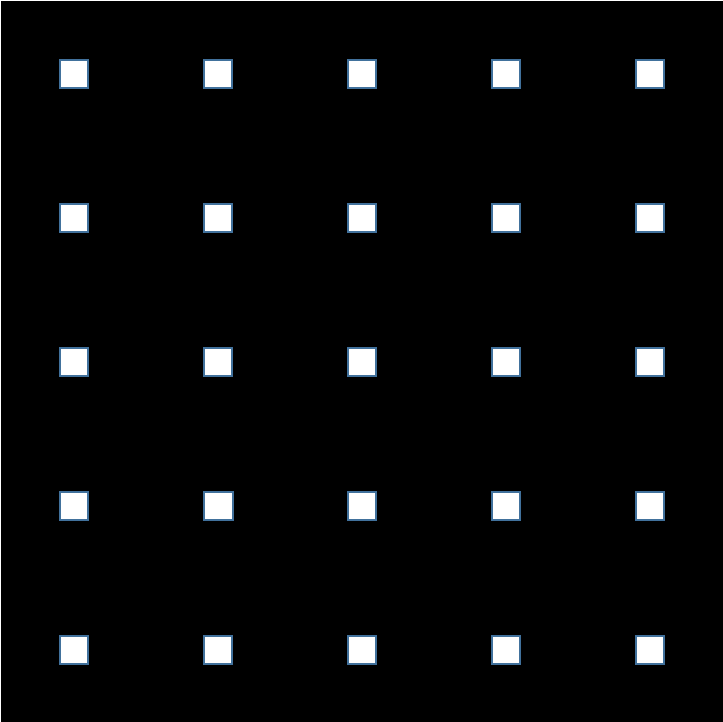
\includegraphics[width=3.5in]{chapters/chapter3/images/pmask.png}
  \caption{Area blocked and covered by pinhole.}
  \label{fig:pinhole}
\end{figure}

The pinhole mask is an example of a parallax barrier. The parallax barrier attenuates most of the light rays in the area covered by the pinhole. Therefore, less light rays will interfere, and light from each pixel will land on a smaller area on the retina. The blur as a result of defocus is reduced and contrast is improved. 

\begin{figure}[ht]
  \centering
  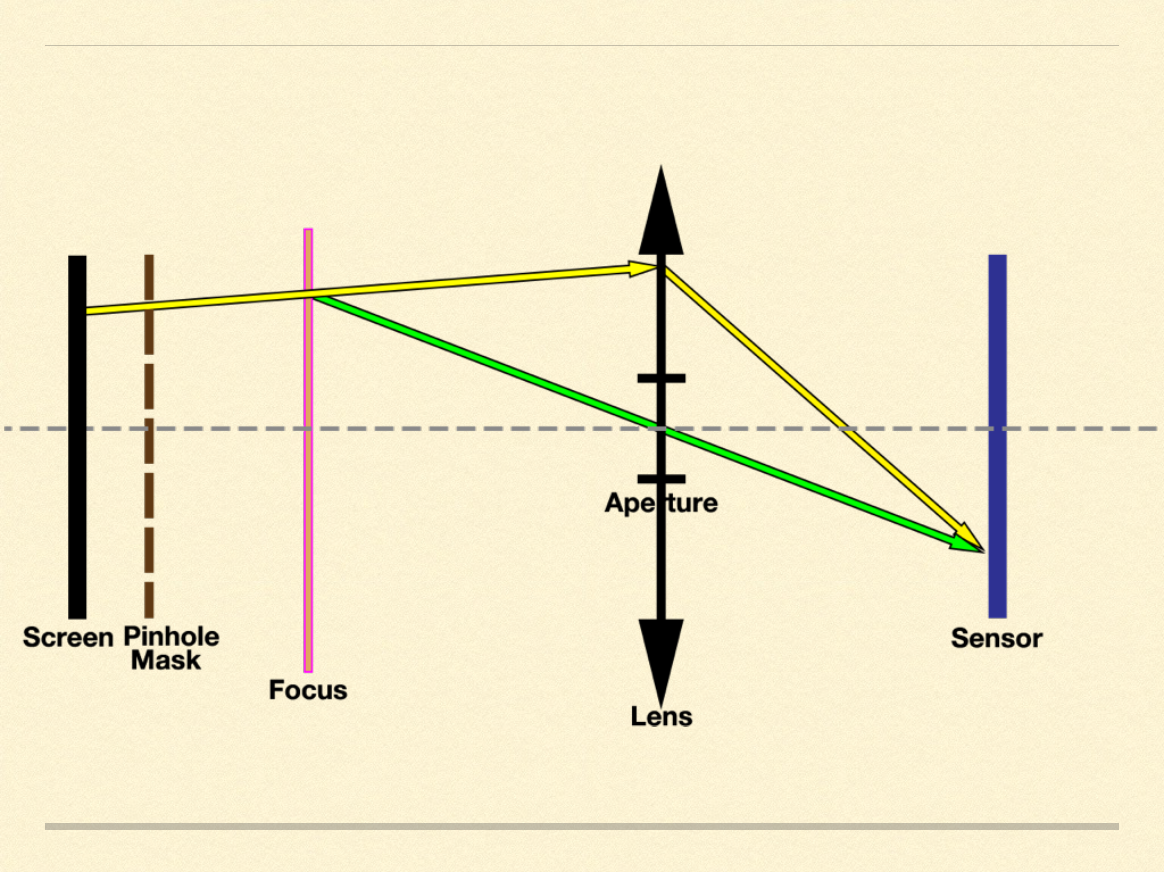
\includegraphics[width=5.0in]{chapters/chapter3/images/pinhole_rays.png}
  \caption{Light rays traveling through a pinhole \cite{Wu:EECS-2016-67}}
  \label{fig:pinhole_light}
\end{figure}

Previously, Huang et al. 2014 \cite{Huang:2014:VisionCorrectingDisplay} developed a similar pinhole mask display. Both Huang's display and our display had pinholes of size 75 micrometers that are 390 micrometers apart. Huang's display is used for the Apple iPod touch 4th generation display, which has a pixel pitch of 78 micrometers and resolution of $960 \times 640$ pixels, while our display is used for the iPhone 6, which has a resolution of $1334 \times 750$ pixels. Our pinhole mask has a greater depth (6 mm instead of 4 mm), and this increased depth allowed the outer pixels in the $5x5$ superpixel covered by the pinhole to become more visible. The light rays from the outer pixels travel at an angle through the pinhole mask and will miss the pupil or aperture if the angle was too large.


\section{Lens Array Display}

The lens array display is a 2D array of microlenses etched on a layer semiconductor material. A microlens is a small lens, generally with a diameter less than a millimeter ($mm$) and often as small as 10 micrometers ($\mu m$). The depth of the microlens is equal to the its focal length so that all of the light rays emanating from a screen pixel travel outwards in parallel. The size of the microlens is equal the length of its covered superpixel. For example, in a 5x5 superpixel on the iPhone6 (pixel size $0.078 mm$), the diameter of the microlens would be $5 \times 0.078mm = 0.3895mm$.  

\begin{figure}[ht!]
  \centering
  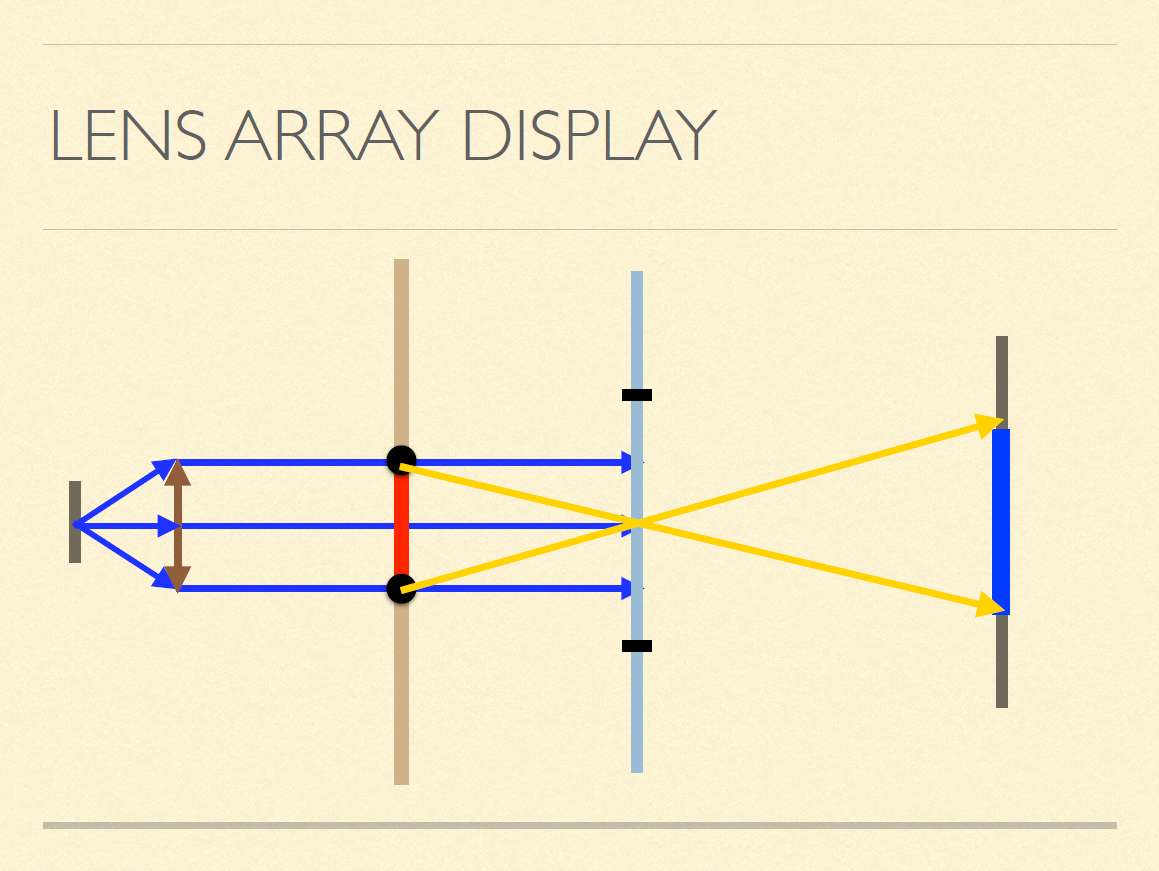
\includegraphics[width=5.0in]{chapters/chapter3/images/lens_rays.png}
  \caption{Light rays traveling through a microlens \cite{Wu:EECS-2016-67}}
  \label{fig:lens}
\end{figure}


One advantage of the lens array is that no light is lost and no information is lost. In the pinhole mask, light from many screen pixels are blocked, and only about 4 percent of all light under a 5x5 superpixel pass through the pinhole. However, in a microlens array, light from every screen pixel is allowed to pass through. One disadvantage of the microlens array is that it costs significantly more to manufacture than the pinhole mask display.



\chapter{Software of the Vision Correction Display}

\section{Introduction to Algorithms}

% Mention more about what Huang did later
Fu-Chun Huang et al. applied light field technology to develop an algorithm that created a sharp image on the display plane \cite{Huang:EECS-2013-206}. The algorithm took into account Peter Wu introduced the forward method and its optimizations \cite{Wu:EECS-2016-67}. Another new algorithm we will introduce is the backward method, which processes an image under the assumption that most light rays that travel through the center of the pinhole or lenslet. The method aims to improve run time compared to Huang's algorithm while taking into consideration more light rays than the forward method. We will use the same definitions, symbols, and content on Huang's algorithm and the optimized forward method in chapter 4 of Wu's paper \cite{Wu:EECS-2016-67} for consistency.

\subsection{Projection and Prefiltering}

Each algorithm in this paper is divided up into two components: the projection relationship and prefiltering. The projection relationship is the mapping relationship from a point on the display to a point on the sensor or retina. The projection relationship depends on the experimental settings such as focal point, object focus, and object distance. Prefiltering is the step in which the content on the display is modified. Prefiltering takes in the projection relationship and the input image and produces a transformed output image.

\subsection{Symbols}

\begin{figure}[ht]
  \centering
  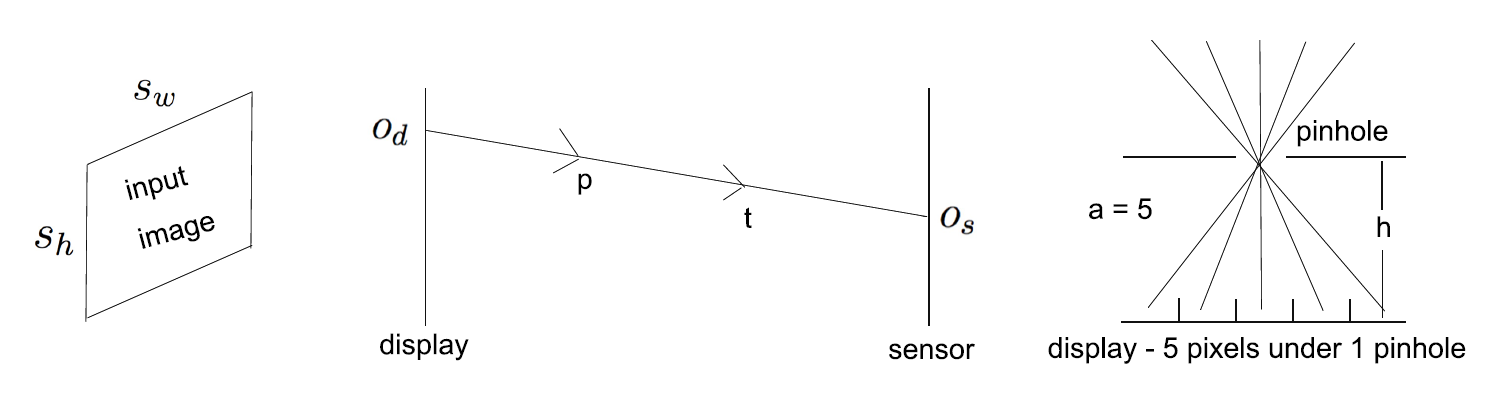
\includegraphics[width=5.0in]{chapters/chapter4/images/Prefilter.png}
  \caption{The figure shows the setup for the prefiltering algorithm. (left) The input image has dimensions $s_w$ by $s_h$ pixels. (middle) $p$ and $t$ are points on the light ray. (right) There are $5$ pixels under each pinhole, and $h$ is the distance between the pinhole and the display. This image is from \cite{Wu:EECS-2016-67}.}
  \label{fig:fr}
\end{figure}


The size of the input image is $s_w$ by $s_h$ pixels. The input image is the unmodified image a normal person sees on the display.
We define two functions $f_s$ and $f_d$, both of which contain the same parameters:
\begin{itemize}
\item $p$ and $t$ stand for arbitrary points in 3-D space. $p$ and $t$ specify a light ray.

\item $e$ is the experimental settings. If we only consider defocus (myopia or hyperopia) the only parameter to consider is the distance from the the screen to the lens.

\item $c$ is the condition of the camera or human eye. If we only consider defocus, then this parameter is the distance from the sensor to the lens.

\end{itemize}

$f_s$ takes in the parameters and computes the position $o_d$, the position where the light ray $(p,t)$ hits the sensor. Similarly, $f_d$ takes in the same parameters and computes the position $o_s$, the position where the light ray $(p, t)$ hits the display. \\
$$f_s(p, t, e, c) \rightarrow O_s$$ \\
$$f_d(p, t, e, c) \rightarrow O_d$$ \\
The angular resolution $a$ is the ratio of the screen resolution to the pinhole mask display or lens array display. \\
The depth $h$ is the distance from the surface of the pinhole mask to the plane of the display.

\section{Huang's Light Field Algorithm}

The projection relation is represented as a matrix in Huang's algorithm. He assumes that the sensor has the same resolution as that of the pinhole mask, which is ($L_s = s_w / a$ by $L_d = s_h / a$). This display pixels have resolution $s_w$ $\times$ $s_h$. 
Next, the algorithm builds a projection matrix. First, an all-zero matrix $P$ with dimensions $L_d$ by $L_s$ is created. Second, for every pixel on the screen, n points $o_n$ are sampled on the aperture, and a light ray $p_s - o_i$ is constructed for each sample point. third, the algorithm applies the function $f_d$ to get the position $p_d$ on the display. Then, the function $m_d$ is called to convert $p_d$ into a 2-D index $I_d$. Finally, algorithms adds index $I_d$ of the matrix by $1/n$. 

After the projection matrix is formed, the following linear equation needs to be solved, where $P$ is the project matrix and $b$ is the one-dimensional representation of the input image:

$$P \cdot x = b$$

$P$ is not a square matrix, but we can multiply both sides by $P^{T}$, and $P^TP$ is square.

$$(P^T \cdot P) \cdot x = p^T \cdot b$$

Define $H = P^T \cdot P$. There is a high chance that $H$ is singular and there is not solution to the linear system. To solve the linear system, a very small positive value $\lambda$ is defined and added to the the system where $I$ is the identity matrix:

$$H' \leftarrow H + \lambda \cdot I$$

$\lambda$ introduces a negligible amount of error to the system, and $H$ is not singular anymore.

Instead of solving the system directly, Huang's algorithm changes it into an optimization problem: \\
% Cite where Huang got his algorithm

Minimize: $$(H'x - P^Tb)^T \cdot (H'x-P^Tb)$$

the L-BGFS method was used to solve this optimization problem. The final result $x$ may have very large positive or very small negative values, but Huang cut off all values in the range (0, 255). The algorithm was applied for the R, G, and B (red, green, and blue) channels separately.


\section{Forward Method}

In the forward method, we assume that the sensor has the same resolution as the screen, so if the screen has size $640 \times 640$ pixels, then so does the sensor. In addition, the light rays travel from the screen to the sensor instead of from the sensor to the screen.

In the projection step of the algorithm, we compute all possible relationships from each point on the screen to the sensor. the direction of the light ray traveling from the screen to the sensor is taken into consideration

The first step in the algorithm is to the set the sensor image equal to the original perfect image. That ray is then traced to the sensor, and the color on the sensor position $o_s$ is equal to the color on the display position $o_d$. 

The two steps can be merged together in that the projection step and prefiltering step can be completed for each pixel. There are no matrices involved.

\lstset {language=C++}
\begin{lstlisting}[frame=single, caption=Pseudocode For Prefiltering Algorithm]
int[][] sensor_image = origin_image;
int[][] prefiltered_image = new int[sensor_image.height][sensor_image.width];

// Loop through the display image
for (int y_index = 0; y_index < screen_size; y_index++) {
  for (int x_index = 0; x_index < screen_size; x_index++) {
        screen_pos = [x_index, y_index];
        pinhole_pos = find_nearest_pinhole(screen_pos);
        sensor_pos = ray_trace(screen_pos, pinhole_pos, sensor_image);
        prefiltered_image[x_index][y_index] = sensor_image[sensor_pos];
  }
}
\end{lstlisting}


\section{Backward Method}

In the backward method, rays are traced form the sensor to the screen, like in Huang's algorithm. We also assume that the resolution of the sensor and screen are the same. 

The first step in the algorithm is to the set the sensor image equal to the original perfect image and the display image equal to a $s_w \times s_h$ array of zeros. For each sensor pixel $o_d$, a ray is drawn to the center position of the closest pinhole, $o_c$ and screen location $o_d$. If the ray passes through the aperture, then the color on the display image is incremented by the the color on the sensor image. We also keep track of the number of hits on each display position and normalize to keep all values between 0 and 255.

\lstset {language=C++}
\begin{lstlisting}[frame=single, caption=Pseudocode For Prefiltering Algorithm]
int[][] sensor_image = origin_image;
int[][] prefiltered_image = new
int[sensor_image.height][sensor_image.width];

// Loop through the display image
for (int y_index = 0; y_index < screen_size; y_index++) {
  for (int x_index = 0; x_index < screen_size; x_index++) {
    for (int py = 0; py < pinhole_size; py++) {
      for (int px = 0; px < pinhole_size; px++) {
        pinhole_pos = compute_pinhole_pos(px, py);
        aperture_pos = compute_aperture_pos(pinhole_pos, 
        x_index, y_index);
        if (aperture_pos.length < aperture_radius) {
          display_pos = compute_display_pos(pinhole_pos, aperture_pos)
          prefilter_image[display_pos] +=  sensor_image[x_index][y_index];
        }
      }
    }
  }
}
\end{lstlisting}


% Insert images here

\chapter{Physical Experiment}

The simulation software in Wu's paper demonstrates that Huang's algorithm and the forward method do a lot to correct for defocus, but does the physical setup yield similar results \cite{Wu:EECS-2016-67}? One can think of the simulation software as tests or a rough draft of a final paper, and the physical demonstration as the final product or copy. The camera in the physical demonstration mimics a human eye with defocus in the real world, and the images captured by the camera are similar to the images perceived by the retina. We set up the camera as a defocused eye and compare the performance Huang's algorithm and the forward method for effectiveness in vision correction.

\section{Physical Setup}

Here is the physical setup used in our experiment: 

\begin{figure}[ht]
  \centering
  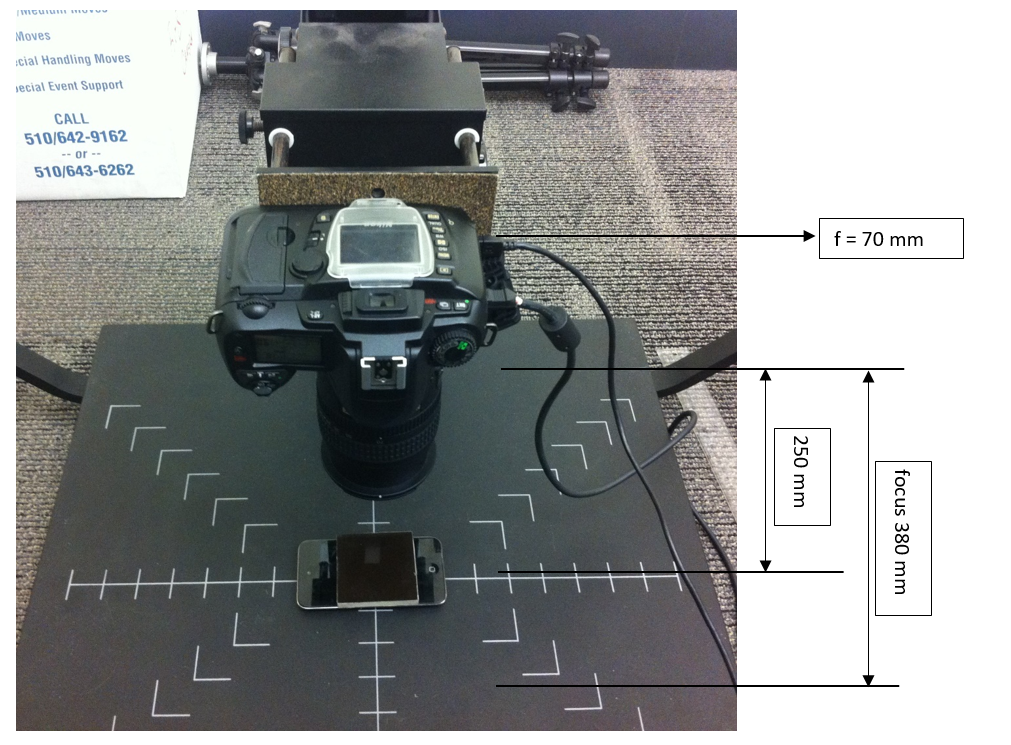
\includegraphics[width=5in]{chapters/chapter5/images/Setup.png}
  \caption{Experimental Setup}
  \label{fig:physical_setup}
\end{figure}
 
The camera used in the experiment was a Nikon D70s digital camera with a Nikon 18-70mm f/3.5-4.5 AF-S DX lens. We set the f-stop of the camera to f/8 (closest to human pupil size of 6 mm), and set the zoom to 70 mm. The distance between the sensor and the flange focal distance, or distance from the flange (the rear end of the lens) to the film plane, is 46.5 mm. The camera was focused at 380 millimeters and the distance between the camera and the phone was 250 millimeters. Since the camera focuses farther than the object, our setup simulates mild hyperopia. We chose such distances to mimic a hyperopic person trying to read from a screen up close. This setup closely resembles a +7.69 D defocus, and a +4.5 D defocus represents a risk factor for adults \cite{iscreenvision.com}. For Huang’s algorithm, the depth of the pinhole mask was 4 millimeters, and for the forward method, the depth was 6 millimeters. Other parameters remained the same for both algorithms. 

\section{Results} 

\begin{table}[!h]
    \caption{Original Images for Reference}
    \begin{tabular}{| l | l }
    \hline Bunny Image & Word Image \\ \hline
      
\includegraphics[width=3in]{chapters/chapter5/images/Clean_Images/0084_820.png} &
      
\includegraphics[width=3in]{chapters/chapter5/images/Clean_Images/Hello.png} \\ \hline
    \end{tabular}
\end{table}


\begin{table}[!h]
    \caption {Huang's Algorithm, Bunny Image}
    \begin{tabular}{| l | l | l |}
    \hline Blurred/Defocused Image & Prefiltered Image & Pinhole-Corrected Image \\ \hline
      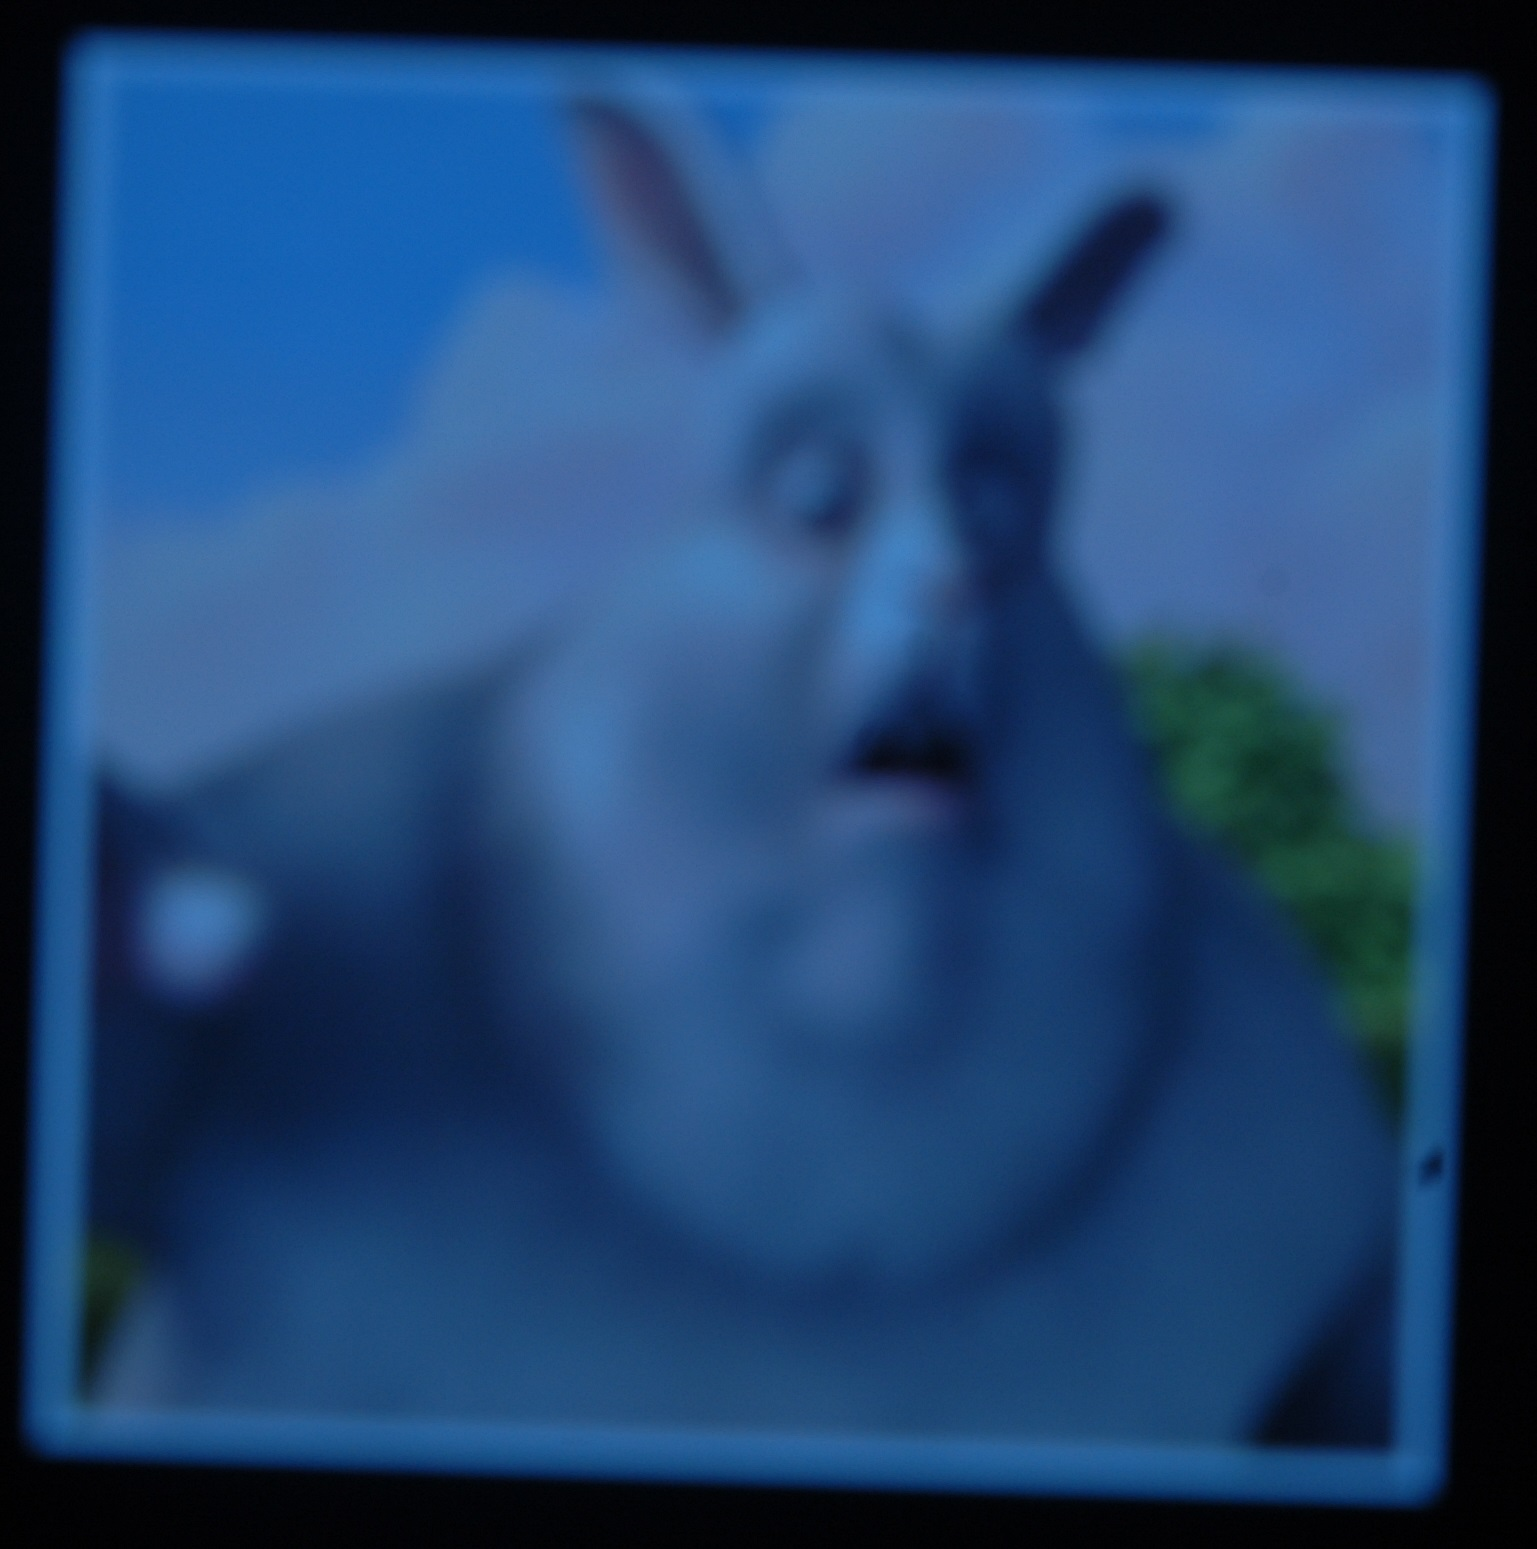
\includegraphics[width=1.9in]{chapters/chapter5/images/Huang_OffAxis_380_250_Origin_Bunny.JPG} &
      \includegraphics[width=1.9in]{chapters/chapter5/images/Huang_prefiltered.PNG} &
      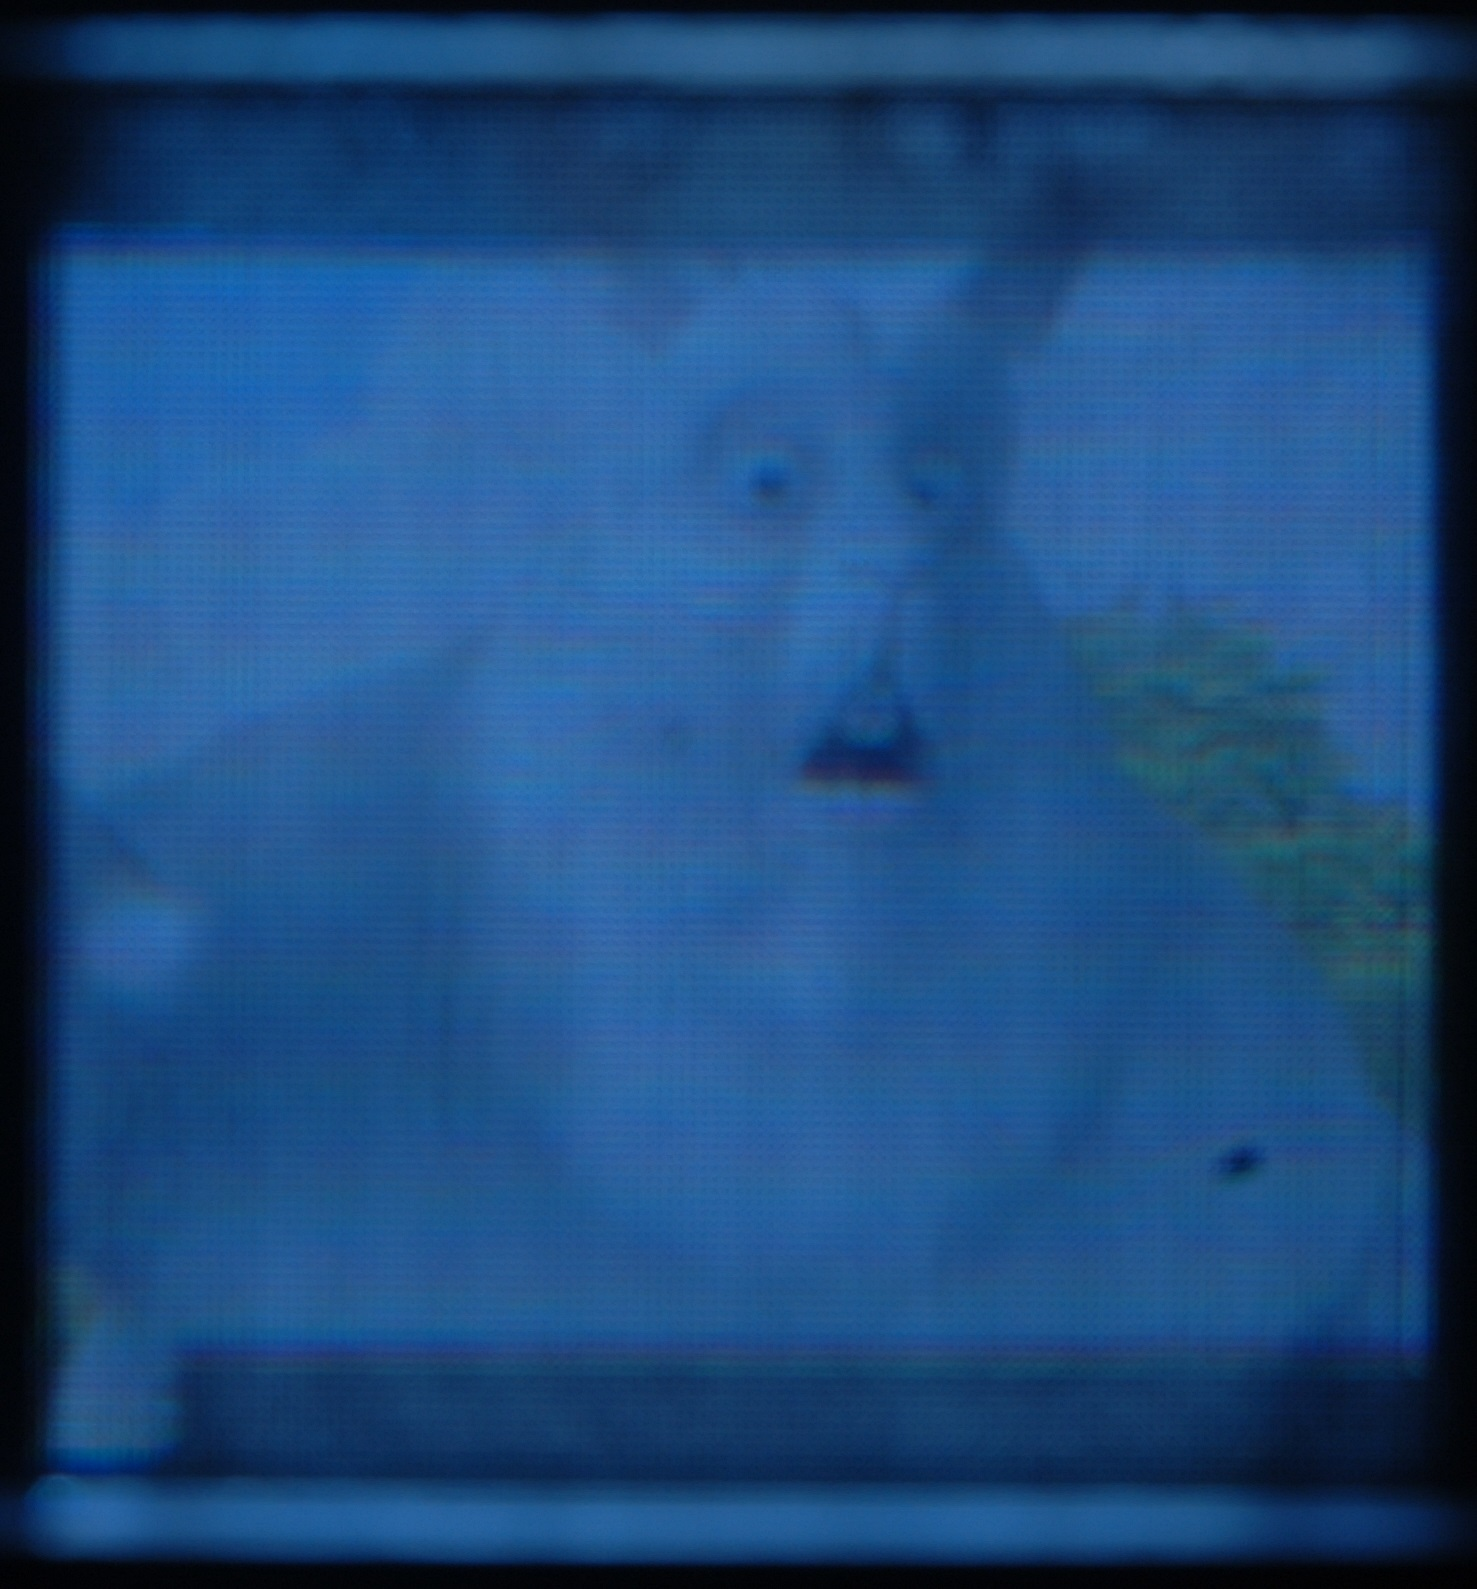
\includegraphics[width=1.9in]{chapters/chapter5/images/Huang_OffAxis_380_250_Pinhole_Bunny.JPG} \\ \hline
    \end{tabular}
\end{table}

\begin{table}
     \caption {Forward Method, Bunny Image}
    \begin{tabular}{| l | l | l |}
    \hline Blurred/Defocused Image & Prefiltered Image & Pinhole-Corrected Image \\ \hline
      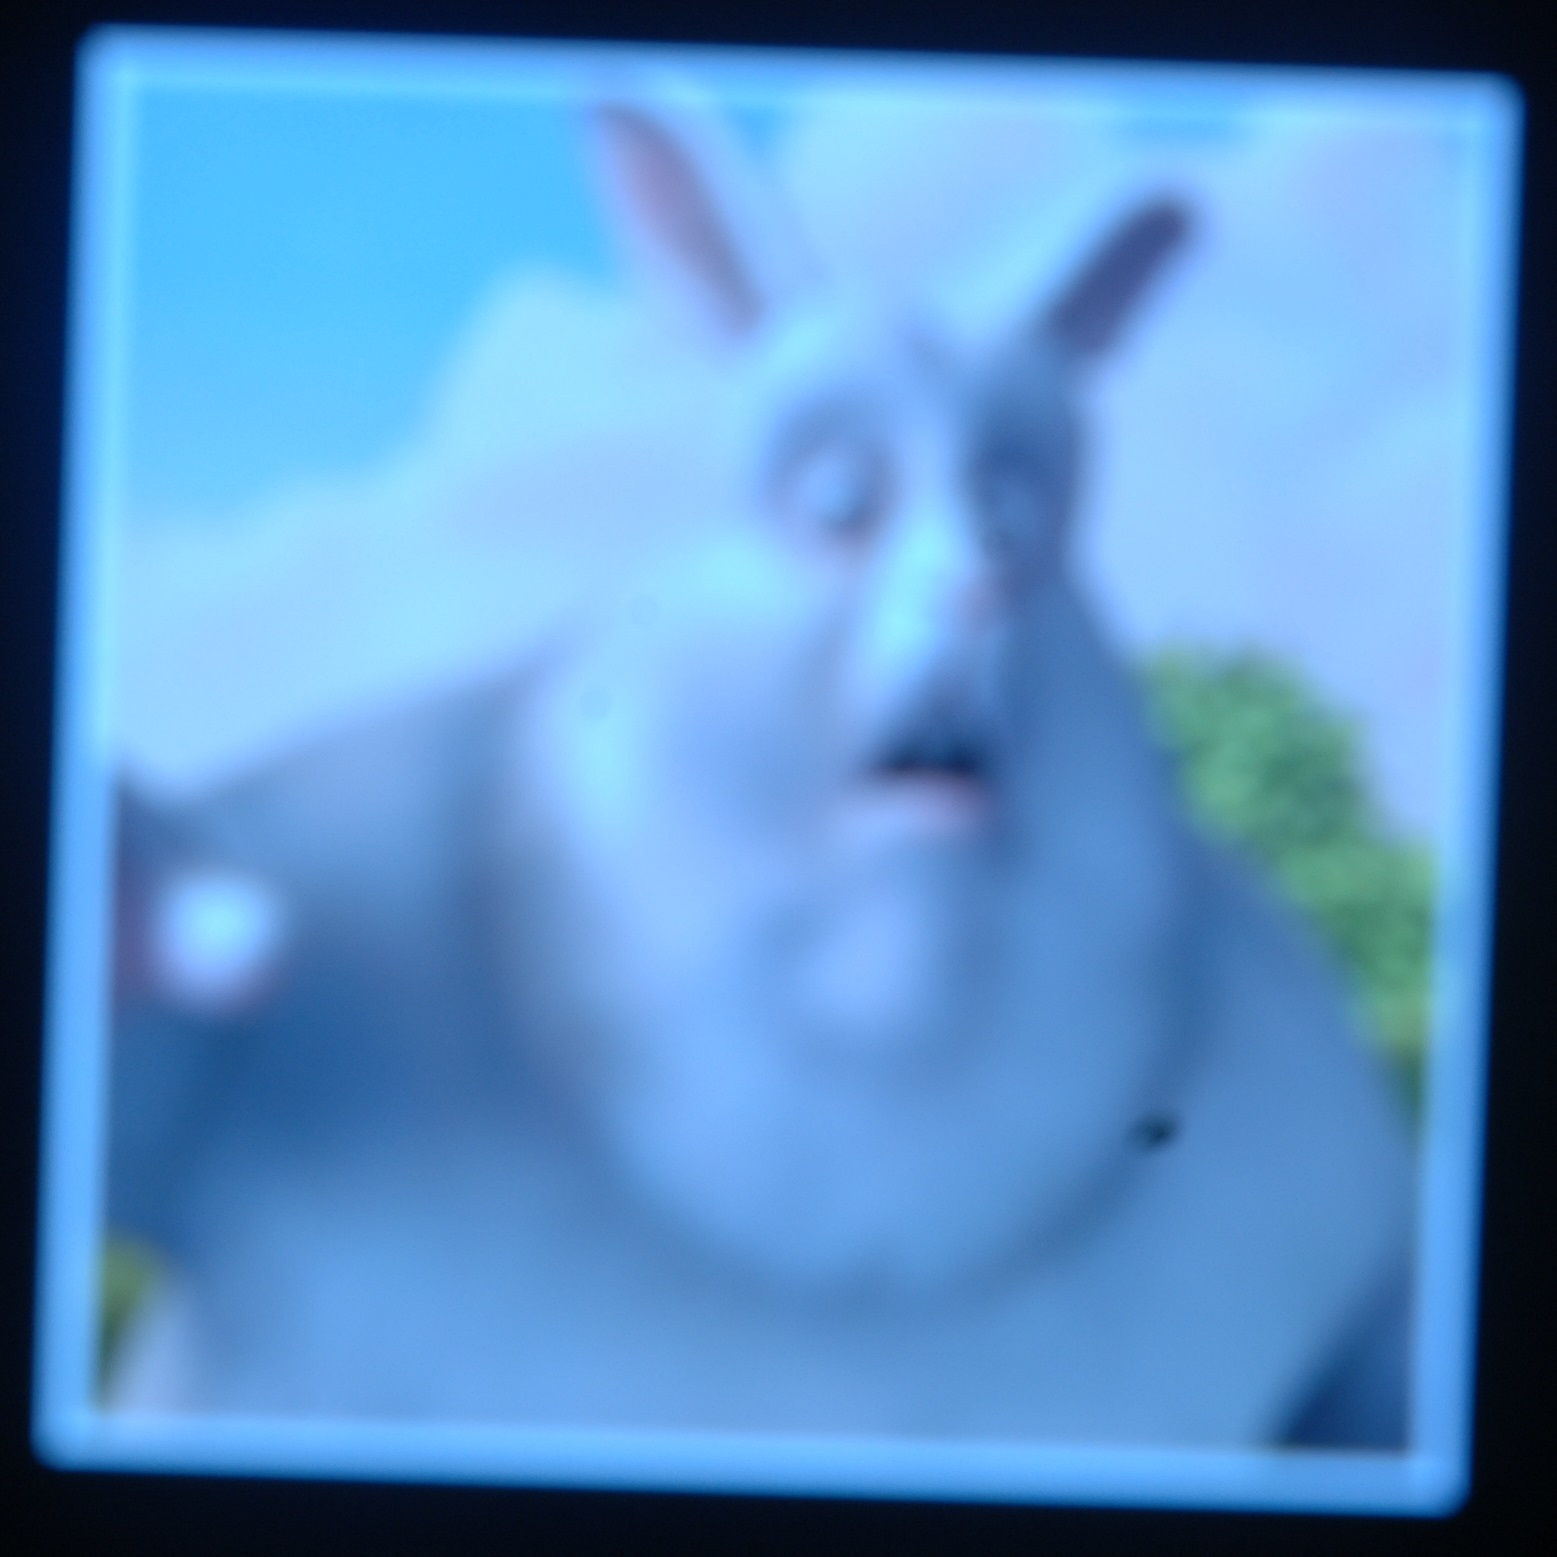
\includegraphics[width=1.9in]{chapters/chapter5/images/Shichao_Bunny_380_250_Origin.JPG} &
      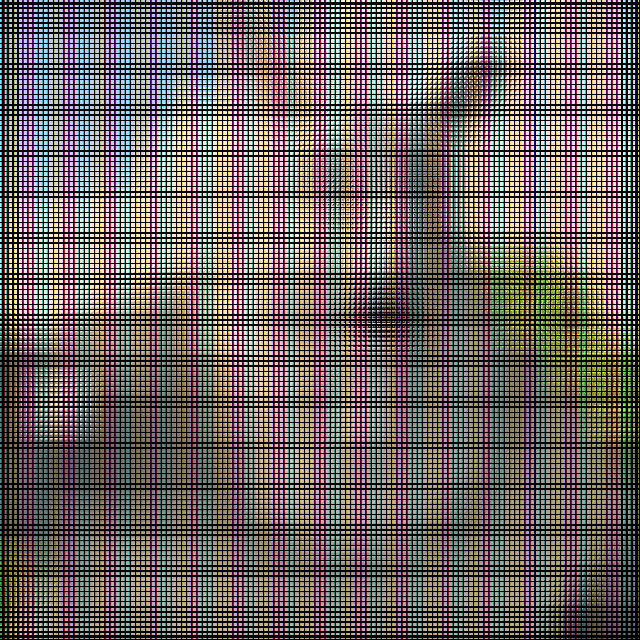
\includegraphics[width=1.9in]{chapters/chapter5/images/Shichao_Bunny_Prefiltered.png} &
      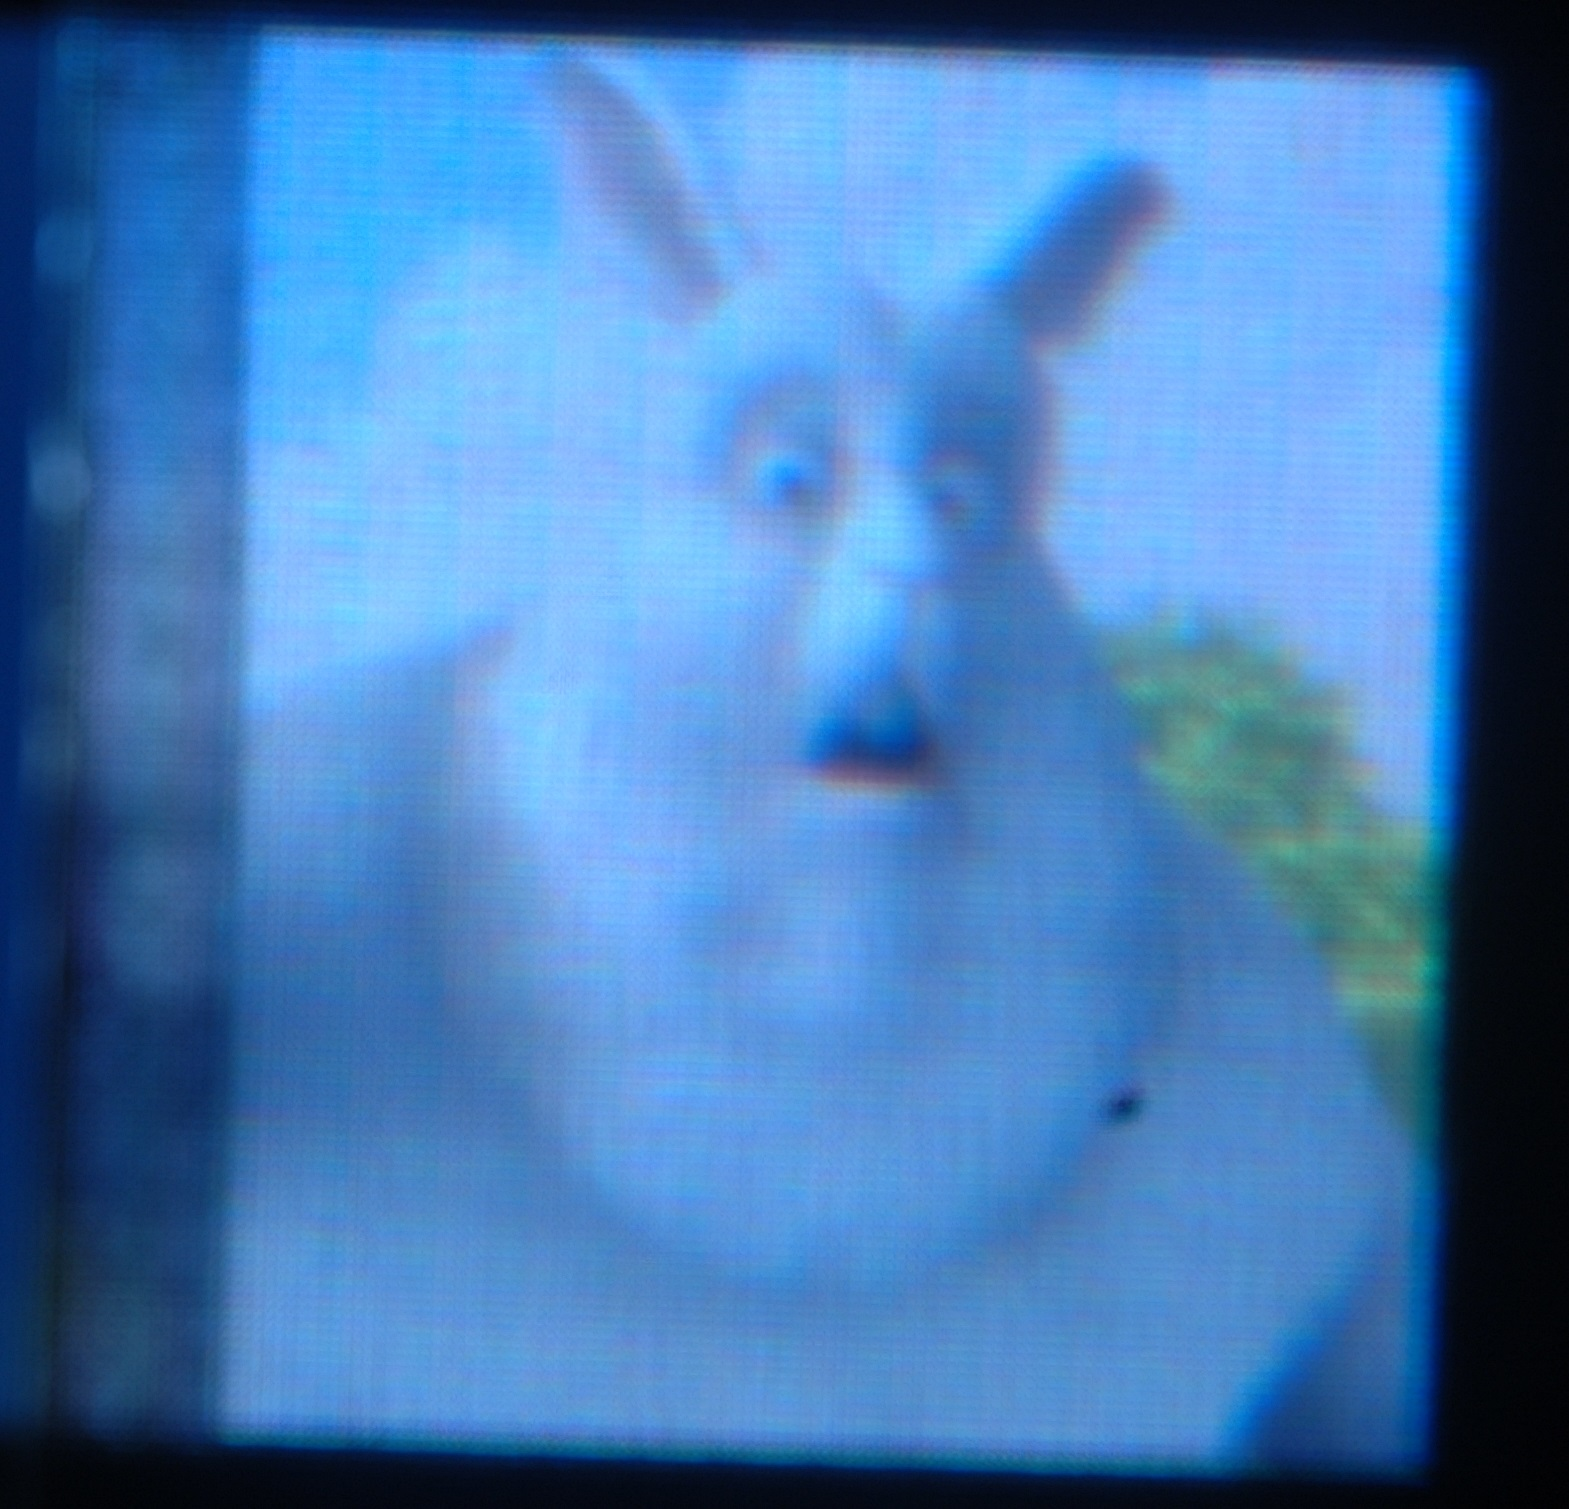
\includegraphics[width=1.9in]{chapters/chapter5/images/Shichao_Bunny_380_250_Pinhole.JPG} \\ \hline
    \end{tabular}
\end{table}
 	 	 
\begin{table}
    \caption {Forward Method, Text Image}
    \begin{tabular}{| l | l | l |}
    \hline Blurred/Defocused Image & Prefiltered Image & Pinhole-Corrected Image \\ \hline
      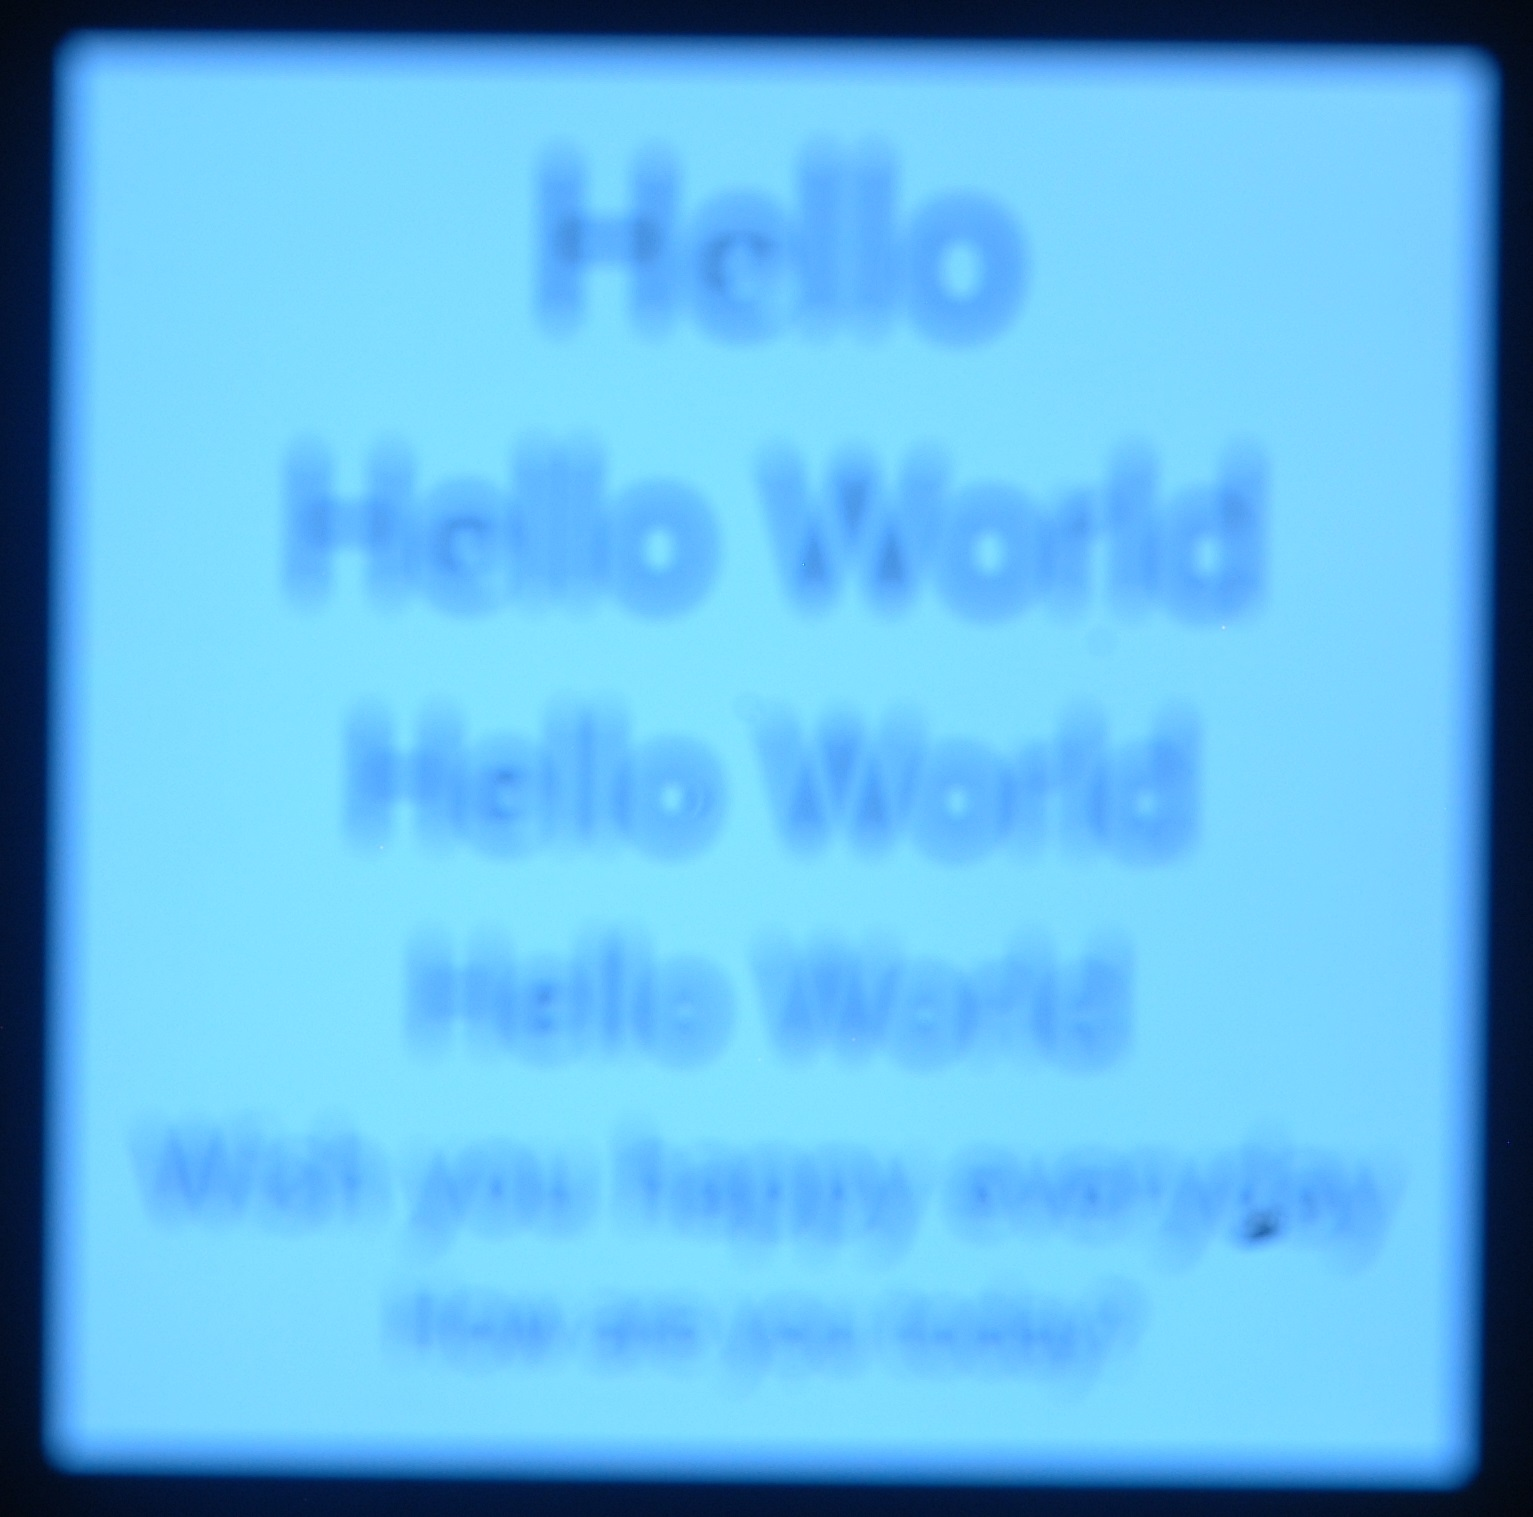
\includegraphics[width=1.9in]{chapters/chapter5/images/Shichao_Words_380_250_Origin.JPG} &
      \includegraphics[width=1.9in]{chapters/chapter5/images/Shichao_word_Prefiltered.png} &
      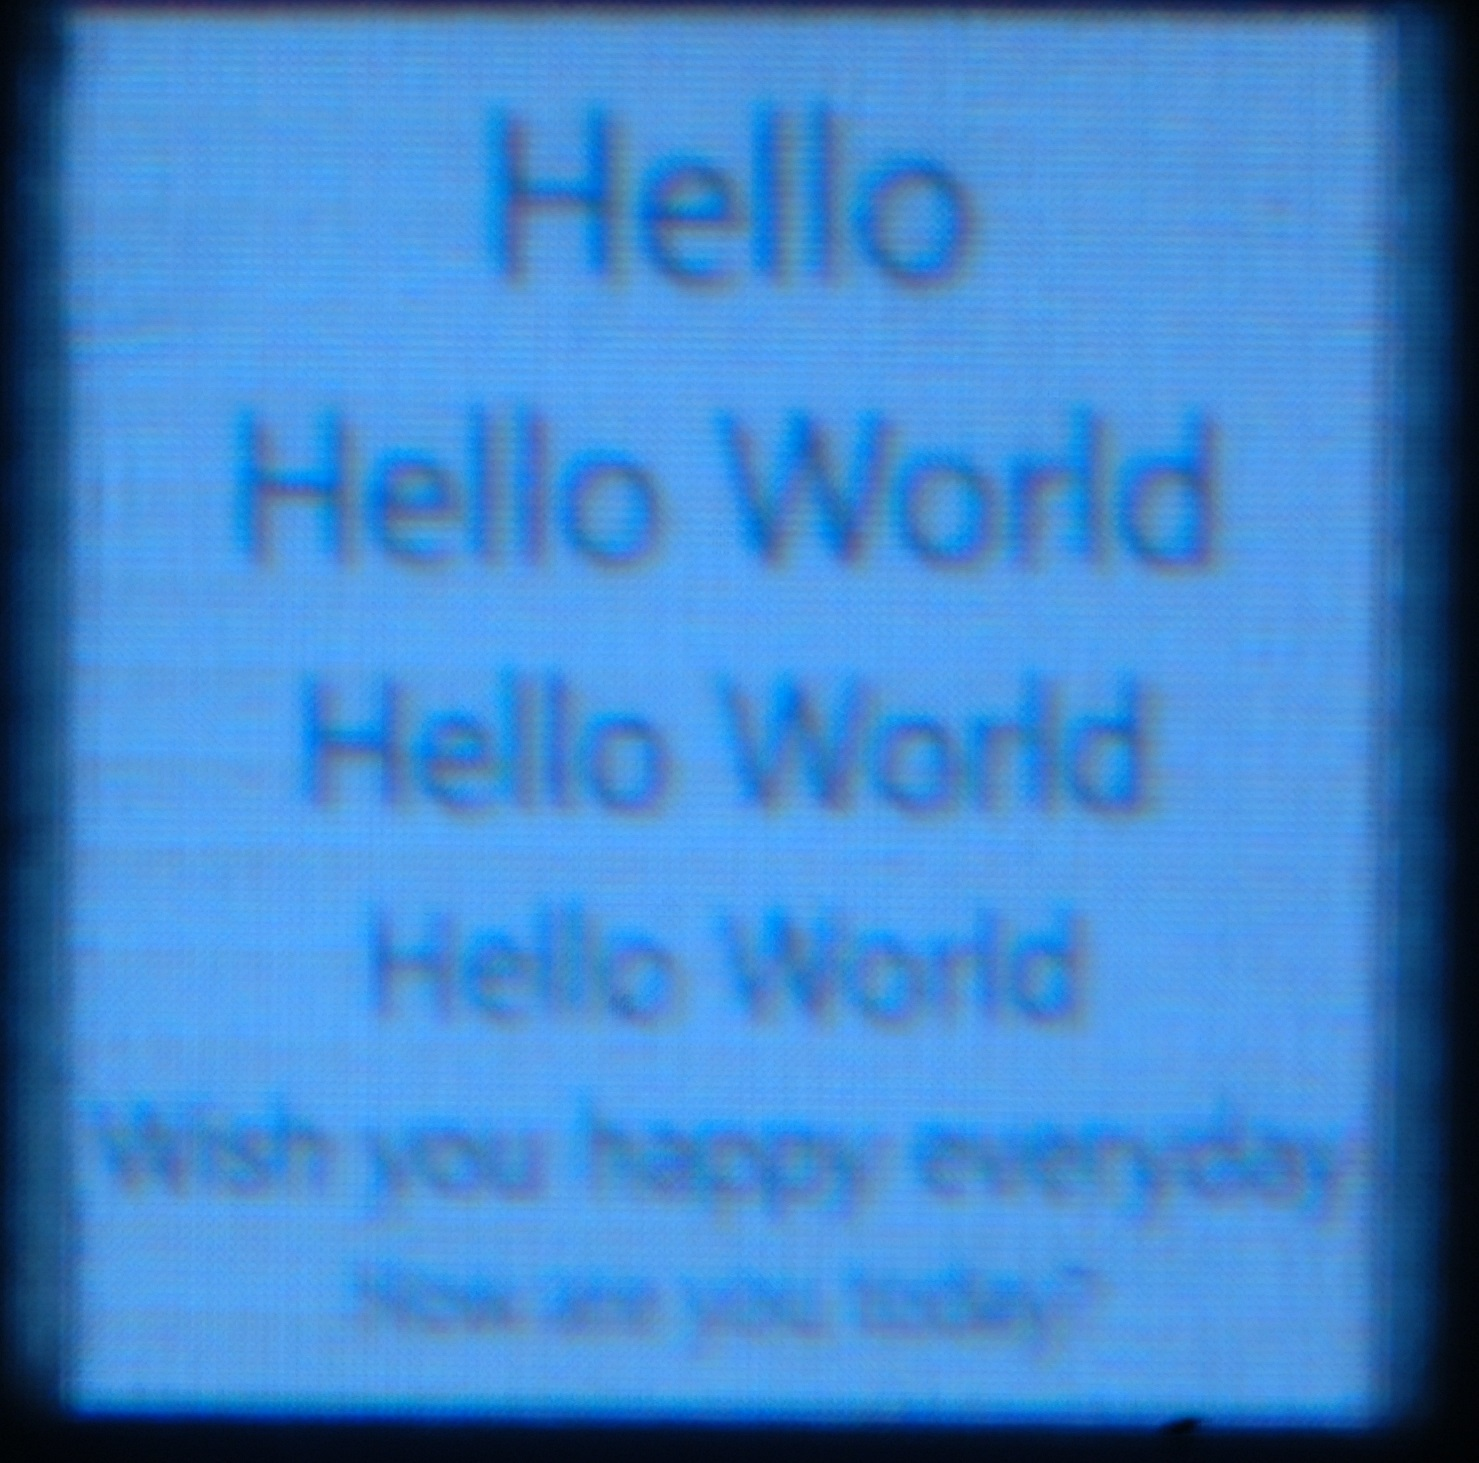
\includegraphics[width=1.9in]{chapters/chapter5/images/Shichao_Words_380_250_Pinhole.JPG} \\ \hline
    \end{tabular}
\end{table} 

\newpage
\section{Analysis}

For Huang’s algorithm, the corrected image shows better resolution but worse contrast. The bunny is far more clear in the corrected image than the defocused image, but the sky becomes saturated. Nevertheless, an average user would likely prefer the corrected image. 

For the forward method, the bunny image shows moderately better resolution with little to no change in contrast. The forward method yields slightly less improvement in resolution than Huang’s algorithm, but the limited loss of contrast makes the forward method more appealing depending on the viewer.

The forward method performs best on the text image in terms of resolution and contrast. In the defocused image, the last three lines are nearly impossible to read, and all words are badly blurred. However, in the corrected image, the first 3 lines are very clear, the next two lines are readable, and only the final line is blurry. 

We adjusted the image brightness on the cell phone and the exposure time of the camera that yielded the best possible results, so we did not keep the brightness factor constant. Nevertheless, exposure time was kept between 1.5 seconds and 2 seconds, so the differences in brightness between images was not significant. In the real world, a user has the ability to adjust the brightness on their cell phone, and a human eye is capable of adjusting to different light conditions. 

\section{Conclusion and Future Work}
For this specific case – an object placed 250 millimeters away and focused at 380 mm – both Huang’s algorithm and the forward method yield improvements in quality of image. In the bunny image, Huang’s algorithm yields slightly better resolution than the forward method but at the cost of losing contrast. The improvement in text image in the forward method is especially appealing because users usually spend more time reading text on an iPhone than viewing images. 
In the future, we want to run experiments on other object distances, focus distances, and depths. For example, we may want to try to simulate myopia (nearsightedness) – focus at 380 mm but place the object 500 mm away. Moreover, we want to do physical experiments with higher-order aberrations, which is much more challenging.

\chapter{Software Simulation}

We develop a software simulation to model the effectiveness of the pinhole mask display. There are multiple motivations for the software simulation. One, a software simulation allows experiment parameters, such as focus distance and physical distance to be adjusted more easily. In addition, a pinhole mask display is costly, and the software simulation is used to fine tune the parameters of the pinhole mask, such as depth and pinhole size. Finally, higher order aberrations are difficult to simulate with ordinary lenses, but Zernike polynomials are easy to incorporate into a software simulation.

\begin{figure}[ht]
  \centering
  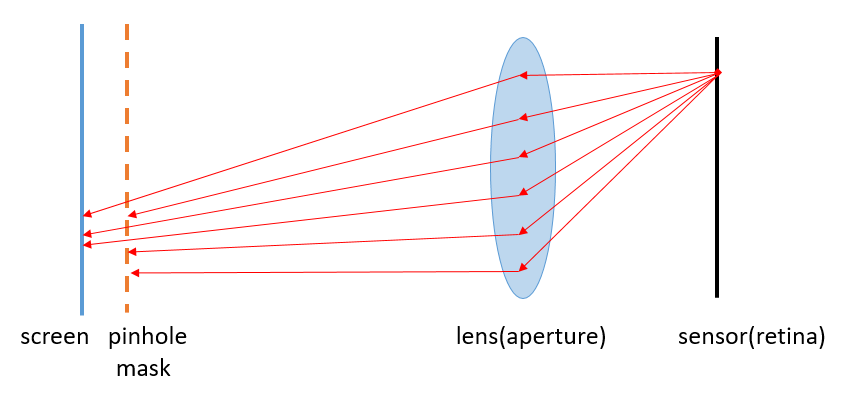
\includegraphics[width=5in]{chapters/chapter6/images/Ray_Simulation.png}
  \caption{Ray Optics Simulation}
  \label{fig:ray_optics}
\end{figure}

One approach we take to simulate the physical experiment is a purely ray optics model. We use a backward ray tracing algorithm, in which light travels from the sensor plane to the display plane. For every pixel on the sensor, the simulation samples multiple points on the aperture (human eye pupil of diameter 6 millimeters). The ray travels straight from the sensor pixel to the aperture point and to the screen. Some of the light rays may get blocked by the pinhole mask or entirely miss the screen. Each screen pixel is composed of a blue, green, and red area, and the color of the ray depends on which position it lands on the screen pixel. Each light ray that reaches the screen contributes to the red, green, or blue intensities of the sensor pixel.

\begin{lstlisting}[frame=single, basicstyle=\footnotesize\ttfamily, caption=Pseudocode For Ray Optics Simulation]
int[][][] sensor = new int[sensor_size][sensor_size][3];
// Iterate over sensor pixels
for (int iy = 0; iy < sensor_size; iy++) {
  for (int ix = 0; ix < sensor_size; ix++) {
    int color[3] = {0, 0, 0};
    int hits = 0;
    // Iterate through random aperture points
    for (int i = 0; i < aperture_sample_time; i++) {
      sensor_pos = (ix, iy);
      aperture_pos = (aperture_samples[2*i], aperture_samples[2*i + 1]);
      type,color = getRayColor(sensor_pos, aperture_pos);
      if (value >= 0) {
        hits++;
	color[type] += value;
      }
    }
  }
  sensor[ix][iy] = color * 3 / hits;
}
\end{lstlisting}

In the physical world, each pixel of light travels straight through free space, through the pupil, and hits a point (rod or cone cell) the retina. Each point on the retina may receive light rays from multiple pixels, so the backward ray tracing algorithm does a good job simulating a human eye. 

Another advantage of this approach is that it is simple and easy to parallelize. With OpenCL, a simulation of an image of size $640\times640$ pixels for roughly $1100$ aperture samples runs in less than one minute. This approach can also take into consideration the quantity of light traveling from the screen to the sensor. If the pinhole size is too small, then too many light rays are blocked by the pinhole mask, and the image on the sensor becomes dim due to the lack of light. To fix this issue, we divided the sum of the light rays by the number of hits. \\
\\
One disadvantage of the ray optics model is that it does not take into account wave properties like diffraction and interference. Even though small pinhole sizes are able to focus light more clearly, they also create larger diffraction effects, which this model does not capture. 

\chapter{Case Study: RGB Pixel Arrangements}

A pixel is composed of miniature red, green, and blue LEDs. When modeled as a square, there is a red, green, and blue component as well as dark areas. Different phones have different RGB pixel arrangements, and we want to test whether the prefiltering algorithm work regardless of pixel arrangement. We ran the software simulation with the forward method on different pixel arrangements. We consider the scenario with no pixel arrangements, which is the same as a RGB order on an OpenCV image, and a base case of a simple red, green, and blue bars, in that order. The different devices that we considered are the iPhone \footnote{Link to iPhone pixel: https://www.androidheadlines.com/2013/04/samsung-shows-off-the-new-diamond-pixel-layout-behind-the-s4s-amoled-display.html \cite{android:headlines}} and three generations of Samsung \footnote{Link to Samsung Galaxy S2 pixel: http://www.gsmarena.com/samsung\_galaxy\_note\_ii-review-811p3.php \cite{gsmarena}} \footnote{Link to Samsung Galaxy S3 pixel: https://www.androidheadlines.com/2013/04/samsung-shows-off-the-new-diamond-pixel-layout-behind-the-s4s-amoled-display.html \cite{android:headlines}}  \footnote{Link to Samsung Galaxy S4 pixel: https://www.chipworks.com/ko/node/126 \cite{chipworks}}. We chose a focus at 400 mm, distance of 350 mm, and a screen size of 640x640 pixels. In addition, for the simulation, we compared normalizing by total number of hits and normalizing by the number of hits per color.

\section{Results}

% TODO: rerun no pixel arrangement with pixel size = 78 micrometers
% TODO: rerun pixel arrangement with bug fixed just to see if there is a difference

\begin{figure}
    \centering
    \textbf{No Pixel Arrangements}\par\medskip
    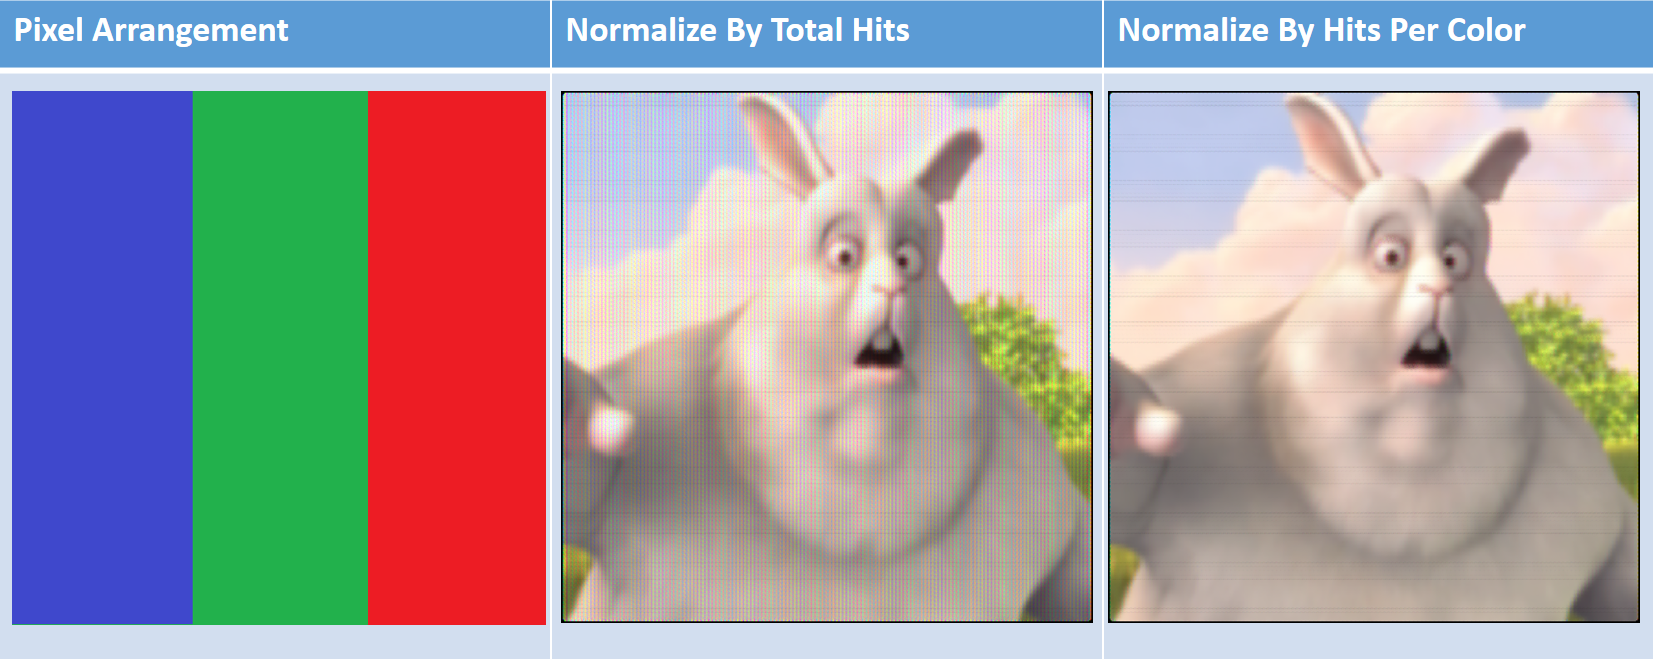
\includegraphics[width=6in]{chapters/chapter7/images/No_Pixel_Arrangement.png}
\end{figure}

\begin{figure}
    \centering
    \textbf{Base Case: RGB Bar}\par\medskip
    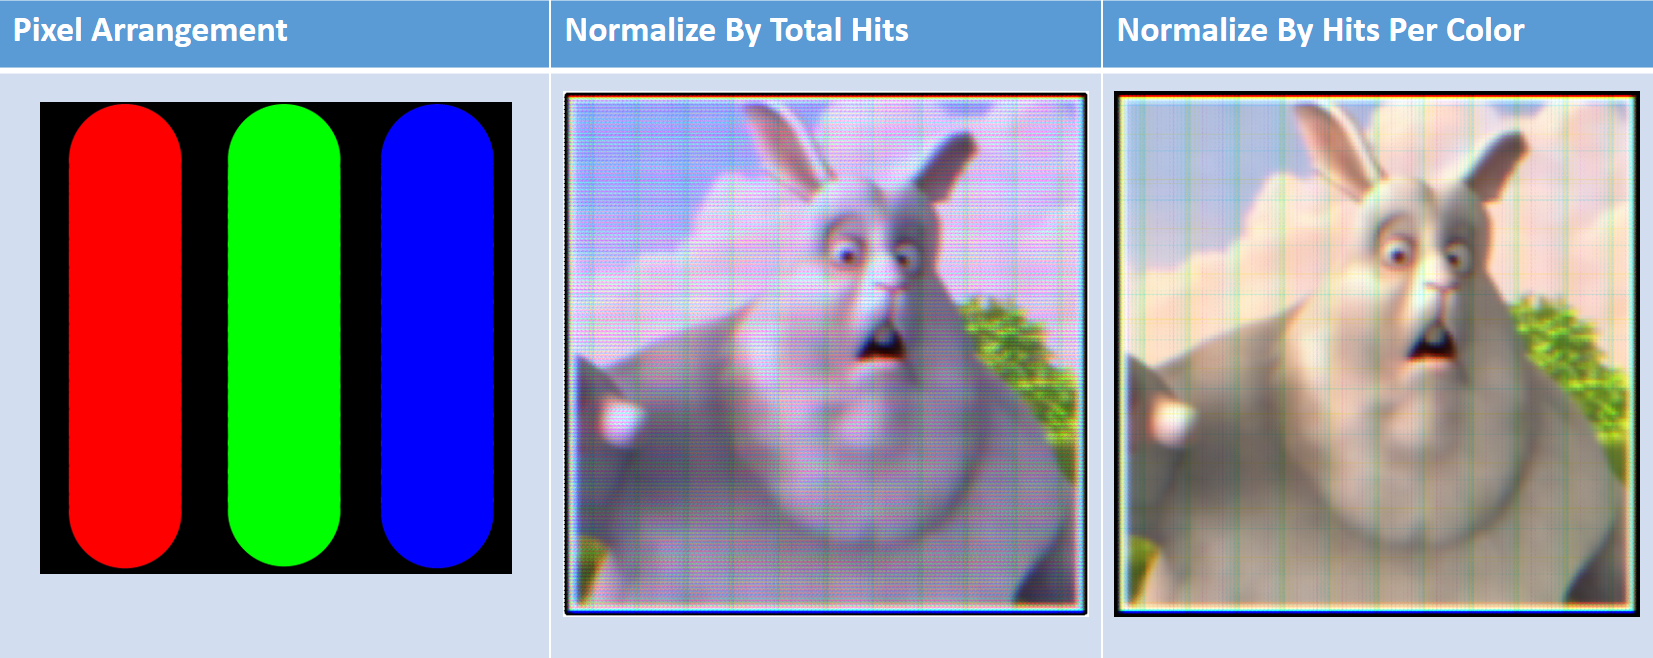
\includegraphics[width=6in]{chapters/chapter7/images/RGB_Bar.png}
\end{figure}

\begin{figure}
    \centering
    \textbf{iPhone}\par\medskip
    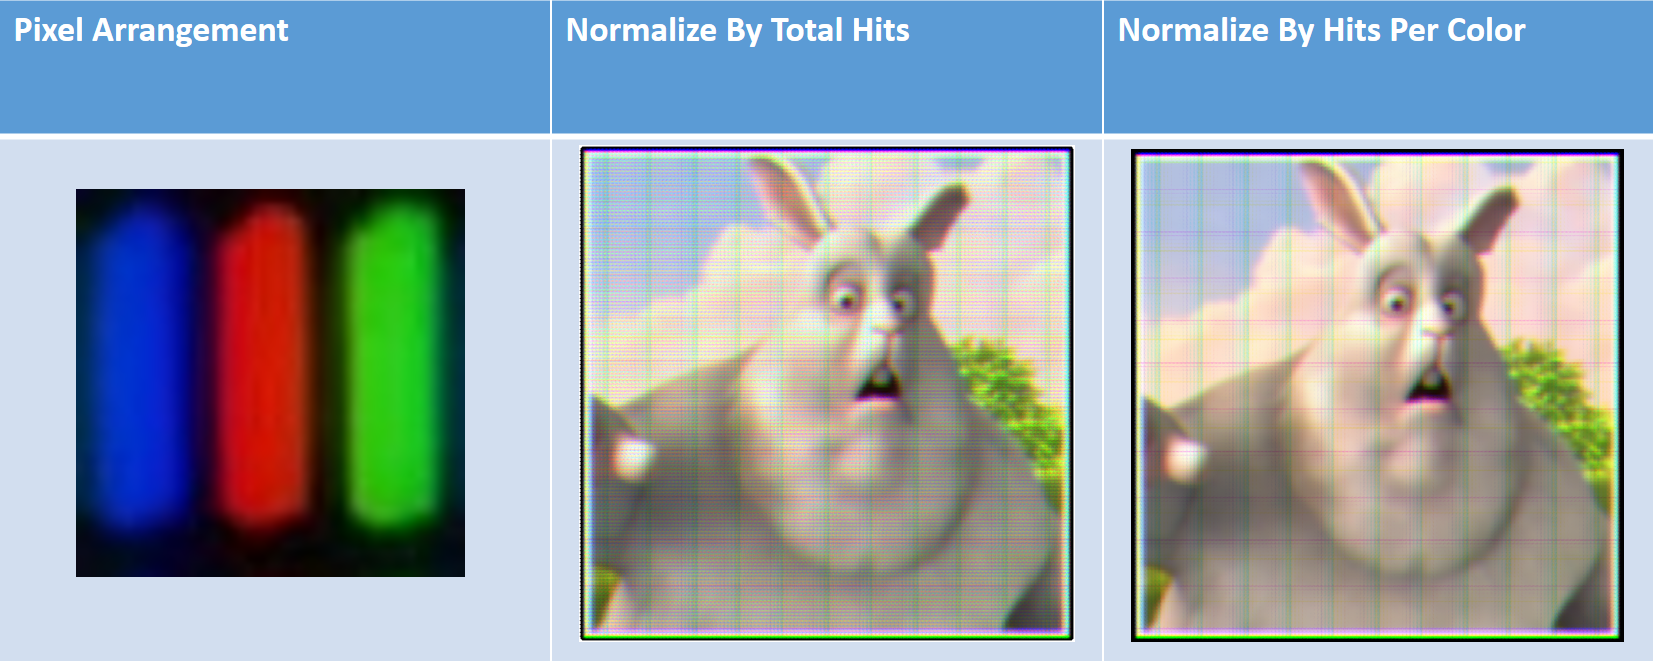
\includegraphics[width=6in]{chapters/chapter7/images/iPhone.png}
\end{figure}

\begin{figure}
    \centering
    \textbf{Samsung Galaxy S2}\par\medskip
    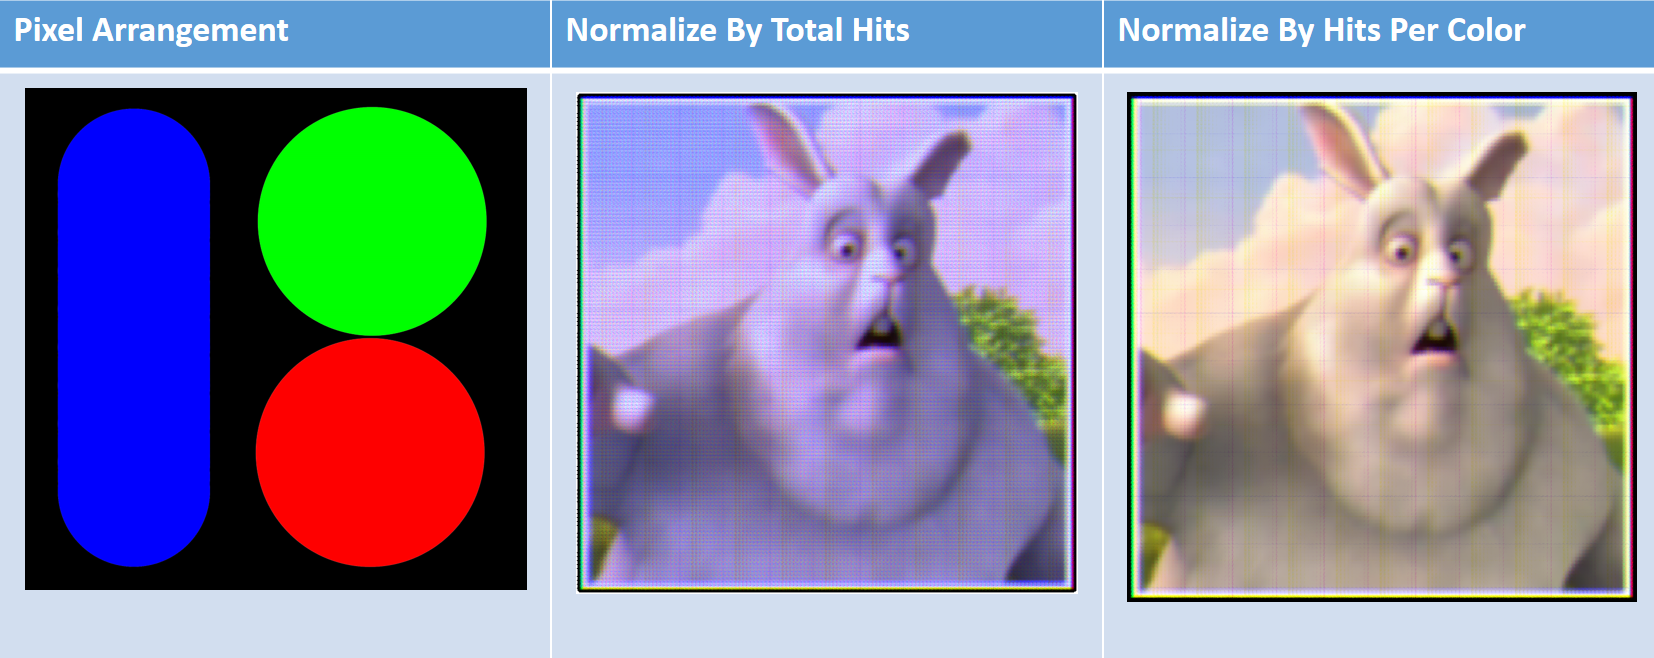
\includegraphics[width=6in]{chapters/chapter7/images/Samsung_Galaxy_S2.png}
\end{figure}

\begin{figure}
    \centering
    \textbf{Samsung Galaxy S3}\par\medskip
    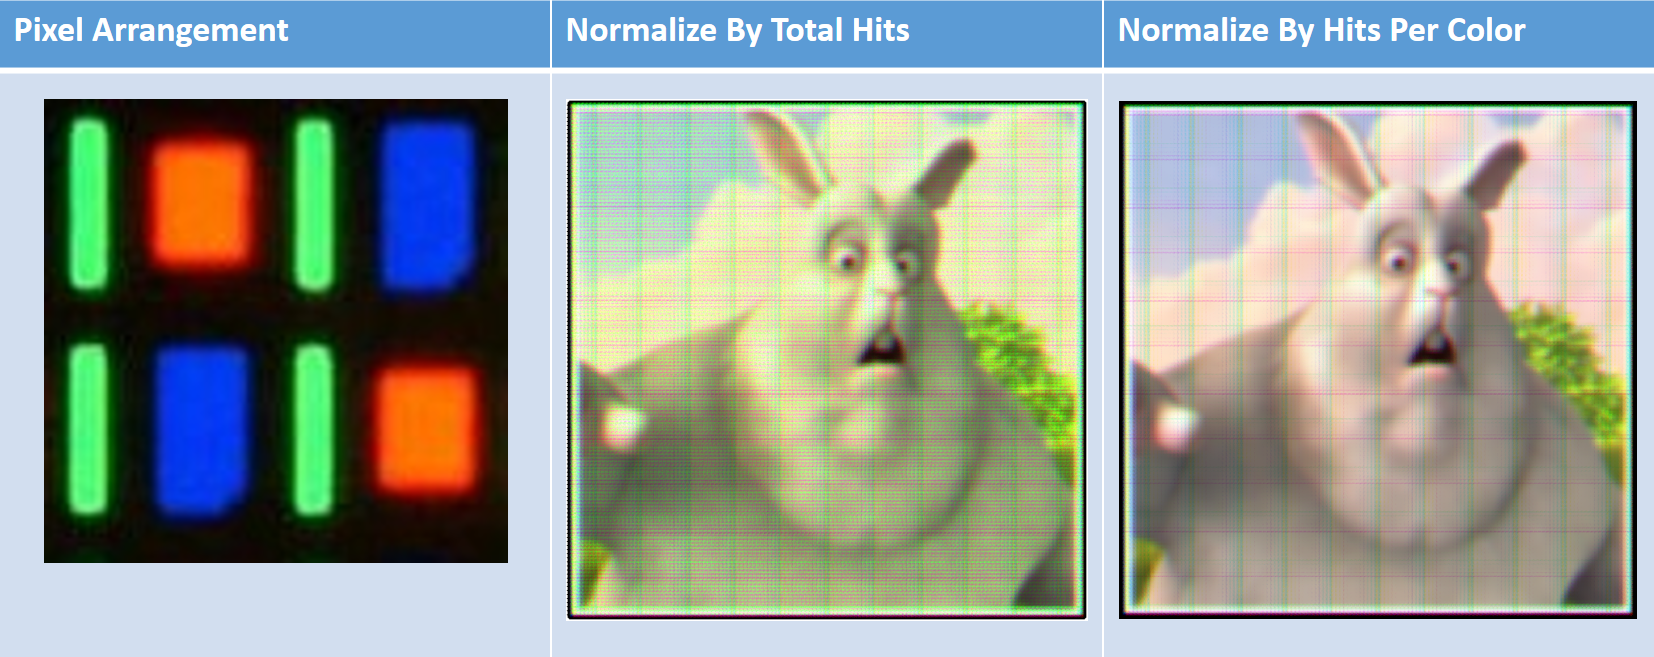
\includegraphics[width=6in]{chapters/chapter7/images/Samsung_Galaxy_S3.png}
\end{figure}

\begin{figure}
    \centering
    \textbf{Samsung Galaxy S4}\par\medskip
    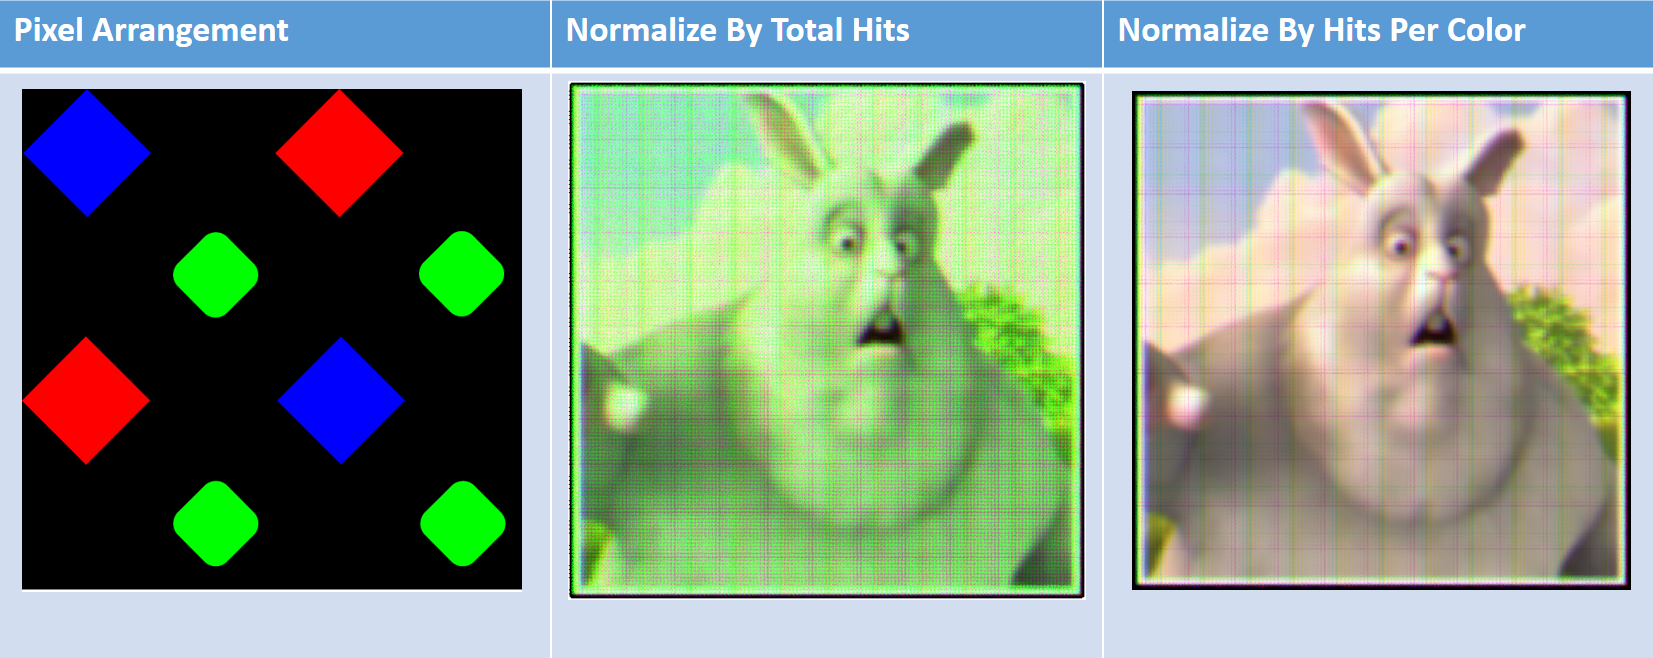
\includegraphics[width=6in]{chapters/chapter7/images/Samsung_Galaxy_S4.png}
\end{figure}

\newpage
\section{Analysis}

The default simulation (OpenCV RGB bars) yields the best results, which is expected. The RGB Bar and the Samsung Galaxy S2 have images that are bright with a blue hue when normalization by the total number of hits is considered. This is expected for the Samsung Galaxy S2 since the the blue LED covers a larger area than the green or red LED, but very unusual for the RGB bar, which has equal red, green, and blue. The iPhone does not have any unique shade, which is expected. The Samsung Galaxy S3 and especially the Samsung Galaxy S4 have a green shade when normalized by the total number of hits, possibly due to a disproportionate amount of green rays as a result of a larger green area on the pixel. All images look very clear when normalized by hits per color and yield a similar grid pattern. The grid pattern is more severe for pixel arrangements with larger dark area as a percentage of total area, which makes sense because more light rays will miss the screen and deviate from the no pixel arrangement case.

% In the future, calculate a percentage of R, G, and B for each pixel arrangement

% In the future, rerun with bug fixed to see if there is any difference

% Also hid the fact that we used 78 micrometer pinhole

% Also missing sources for the pixel arrangements

As expected, the pixel arrangement creates a major impact when we normalize by the total hits because there is a disproportionate amount of red, green, and blue hits when the red, green, and blue components are not equal in area or on different positions of the pixel. However, when we normalize by hits per color, this issue is resolved. The grided pattern may be a result of some pixels on the sensor that have rays traced to unexpected areas on the screen, but it does not interfere much with clear recognition of the bunny.

\chapter{Case Study: Diffraction through the Pinhole}

% MENTION THE CUTOFF OF THE GAUSSIAN FILTER

One question to ask about the vision correcting display is "What is the optimal pinhole size for the pinhole mask?" The regular simulation applies ray optics, which does not take into account properties of light, such as diffraction and interference. We want a new simulation that models the effects of diffraction through a pinhole.

\section{Software Simulation - Wave Optics}

We utilize another approach to the software simulation that considers both light traveling as a ray and the diffraction effects of the pinhole. 

\subsection{Fraunhofer Diffraction through Rectangular Aperture}
\noindent We assume that each light ray emits a spherical wavefront that creates a constant electric field on the pinhole. We consider each screen pixel as a point source, and since the depth of the pinhole mask (6 millimeters) is much larger than the size of the screen pixel (78 micrometers) or the pinhole (75 micrometers), the value of the electric field will not vary significantly between the edges of the pinhole and center of the pinhole. The distance between the pinhole plane and the sensor plane is about 27 centimeters, which is much larger than the size of the sensor, so there is not a large variation in the length of different light rays traveling from the mask to the sensor. The pinholes are squares, and we meet the conditions for Fraunhofer diffraction through a rectangular aperture [Lipson, Lipson, and Lipson, 2011]: 
$$\frac{W^2}{L \times \lambda} \ll 1$$
Here, $W$ is the length of the aperture, $L$ is the distance of the sensor from the aperture, and $\lambda$ is the wavelength. $W$ is at most $125$ micrometers, $L$ is roughly $27$ centimeters, and $\lambda$ is about $500$ nanometers. 

\begin{figure}[ht]
  \centering
  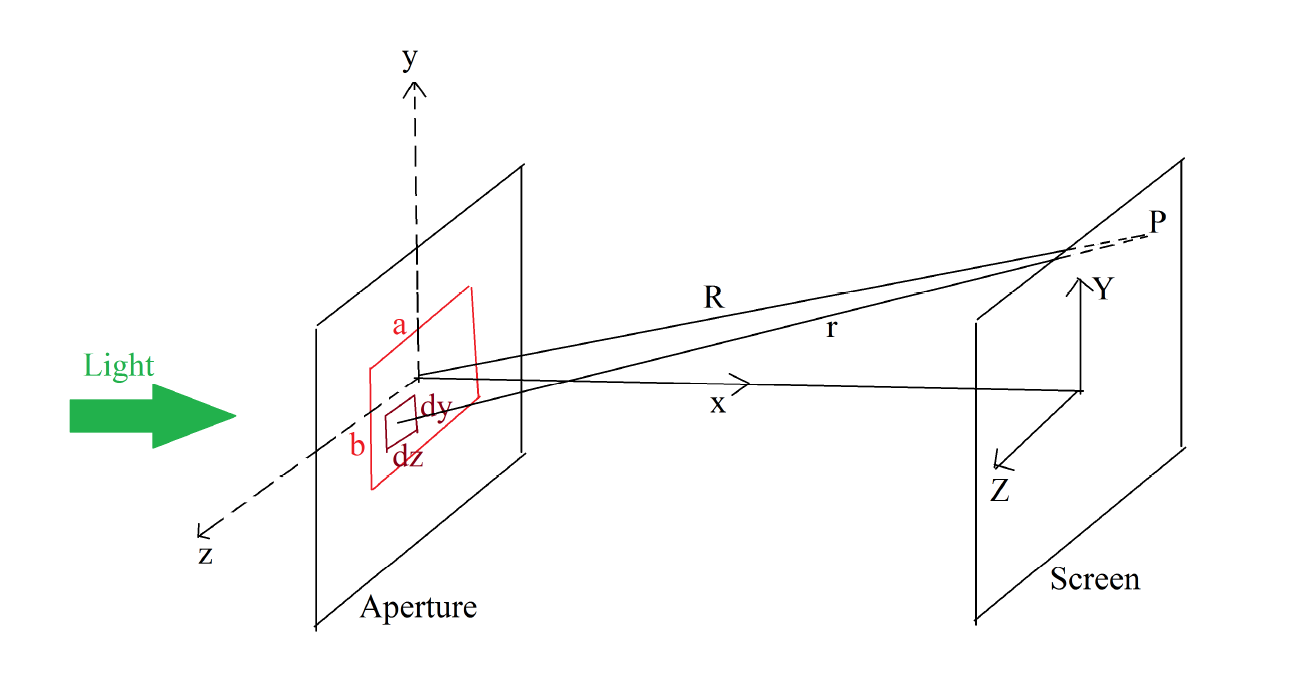
\includegraphics[width=4in]{chapters/chapter8/images/Rectangular_Aperture.png}
  \caption{Fraunhofer Diffraction through Rectangular Aperture Diagram [Rao 2014]}
  \label{fig:ferrari}
\end{figure}

Let $\epsilon_A$ represent the electric field strength per unit area, which is assumed to be constant over the entire aperture (derivation below from Hecht 1987). The electric field contributed by the the small section of the aperture $dzdy$ at point P on the screen is 
$$dE = \left(\frac{\epsilon_A}{R} \right)e^{i(\omega t-kr)}dzdy$$
where $r = [X^2 + (Y-y)^2+(Z-z)^2]^{\frac{1}{2}}$ and $k = \frac{2 \pi}{\lambda}$, the wavenumber. We can use the far field approximation and set $r = R$ for the amplitude term and $r = R[1-(Yy+Zz)^2/{R^2}]$ in the phase term. The total electric field at point $P$ on the screen is \\
$$E = \left(\frac{\epsilon_{A}}{R}\right)e^{i(\omega t-kR)} \int_{-b/2}^{b/2} e^{ikYy/R}dy \int_{-a/2}^{a/2} e^{ikZz/R} dz $$
Solving the integral gives \\
$$E = \left(\frac{ab\epsilon_A}{R}\right) e^{i(\omega t-kR)} sinc\left(\frac{kaZ}{2R}\right)sinc\left(\frac{kbY}{2R}\right) $$ \\
Intensity is equal to the square of the amplitude of the electric field intensity, so \\
$$I(Y,Z) = Re\left[\left(\frac{ab\epsilon_A}{R}\right)e^{i(\omega t - kR)} sinc\left(\frac{kaZ}{2R}\right) sinc\left(\frac{kbY}{2R}\right)\right]^2$$
$$I(Y,Z) = I_0  sinc^2\left(\frac{kaZ}{2R}\right) sinc^2\left(\frac{kbY}{2R}\right)$$
Intensity of light is proportional to two $sinc$ squared functions multiplied in both the $Y$ and $Z$ directions.
% In the future, try to justify your new model.


\subsection{Diffraction through a Lens}
The above diffraction equation creates a very large diffraction pattern on the sensor that leads to far too much loss of contrast. To fix this,we need to consider the effects of the lens and the fact that the display is not placed at the focus distance of 380 millimeters. 

\begin{figure}[ht]
  \centering
  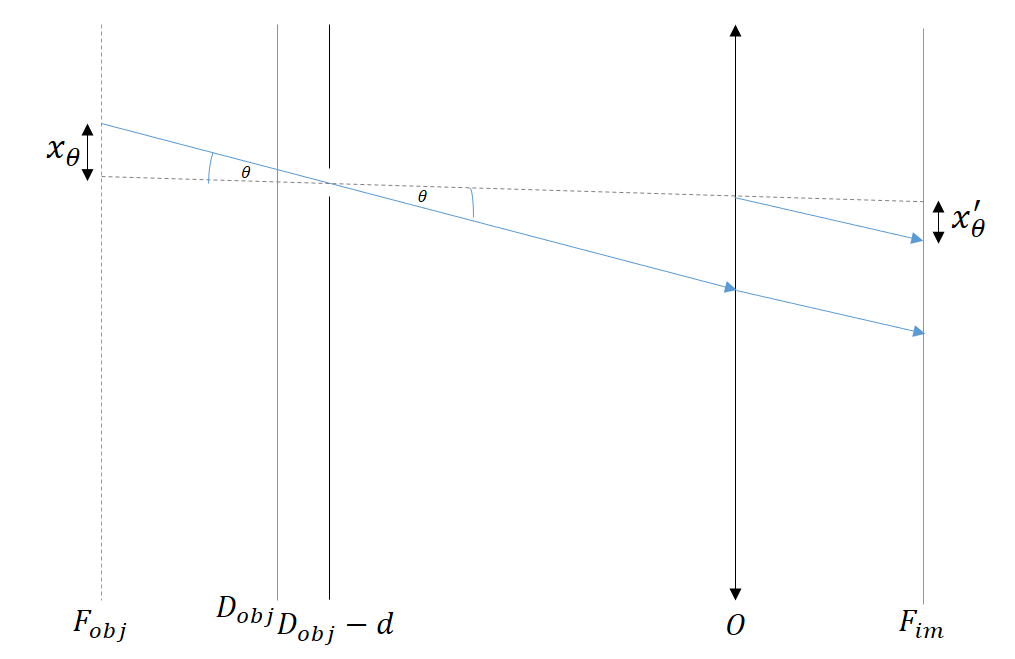
\includegraphics[width=4in]{chapters/chapter8/images/Lens_Diffraction.png}
  \caption{Fraunhofer diffraction through lens. $F_{obj}$ is the focus distance, $D_{obj}$ is the display distance, $d$ is the depth of the pinhole mask, $O$ is the plane of the lens, and $F_{im}$ is equal to position of the sensor at focus.}
  \label{fig:ferrari}
\end{figure}

We know that $$I(Y,Z) = I_0  sinc^2\left(\frac{kaZ}{2R}\right) sinc^2\left(\frac{kbY}{2R}\right)$$
We substitute in $sin(\theta) \sim \frac{Z}{R}$ and $sin(\phi) \sim \frac{Y}{R}$:
$$I(\theta,\phi) = I_0  sinc^2\left(\frac{\pi a sin \theta}{\lambda}\right) sinc^2 \left(\frac{\pi b sin \phi}{\lambda}\right)$$

We want to find the shape of the diffraction pattern as a function of sensor coordinates, $x_{\theta}'$ and $x_{\phi}'$. In other words, we want to determine $I(x_{\theta}', x_{\phi}')$, where $x_{\theta}'$ is the image created by $x_{\theta}$ and $x_{\phi}'$ is the image created by $x_{\phi}$. 

We consider the the angle that light travels through the pinhole, and imagine that the light ray is traced back to the plane at the focus distance. We have: 
$$tan(\theta) = \frac{x_{\theta}}{F_{obj} - D_{obj} + d}$$ 
which gets rearranged to 
$$x_{\theta} = (F_{obj} - D_{obj} + d) tan\theta$$

Then, based on the displacement $x_{\theta}$ on the focus object plane, we can compute the displacement on the sensor $x_{\theta}'$ through the magnification equation. 

$$x_{\theta}' = x_{\theta} \frac{F_{im}}{F_{obj}} =  \frac{F_{im}}{F_{obj}} (F_{obj} - D_{obj} + d) tan\theta $$

Likewise, $$x_{\phi}' = x_{\phi} \frac{F_{im}}{F_{obj}} =  \frac{F_{im}}{F_{obj}} (F_{obj} - D_{obj} + d) tan\phi $$

We want to incorporate the expressions for $x_{\theta}'$ and $x_{\phi}'$ into the original intensity equation. We use the conditions $\theta \ll 1$ (and $\phi \ll 1$) to make the approximations $sin\theta \approx tan\theta \approx \theta$ and $sin\phi \approx tan\phi \approx \phi$. Therefore, 

$$I(\theta, \phi) \approx I_0 sinc^2(\frac{\pi a \theta}{\lambda}) sinc^2(\frac{\pi b \phi}{\lambda})$$

We rearrange $$x_{\theta}' = \frac{F_{im}}{F_{obj}} (F_{obj} - D_{obj} + d) \theta $$ to get $$\theta =  \frac{F_{obj}} {(F_{obj} - D_{obj} + d)F_{im}} x_{\theta}'$$ Likewise,  $$\phi =  \frac{F_{obj}} {(F_{obj} - D_{obj} + d)F_{im}} x_{\phi}'$$ We substitute these results into the intensity equation to get

$$I(x_{\theta}', x_{\phi}') \approx $$ $$I_0 sinc^2 (\frac{\pi a F_{obj} x_{\theta}'}{F_{im}(F_{obj} - D_{obj} + d)\lambda}) sinc^2 (\frac{\pi b F_{obj} x_{\phi}'}{F_{im}(F_{obj} - D_{obj} + d)\lambda})$$

\subsection{Integration of Ray and Wave Optics}

In the integrated ray and wave optics model, ray optics determines the direction of light rays, and wave optics determines the size of the diffraction pattern on the sensor. We continue to do backwards ray tracing on multiple aperture samples, but each ray creates a diffraction pattern on multiple sensor pixels. The combined model is equivalent to blurring the result of the ray optics image by applying a low pass filter, and the blur matrix is determined by the intensities of the diffraction pattern. 

\begin{figure}[ht]
  \centering
  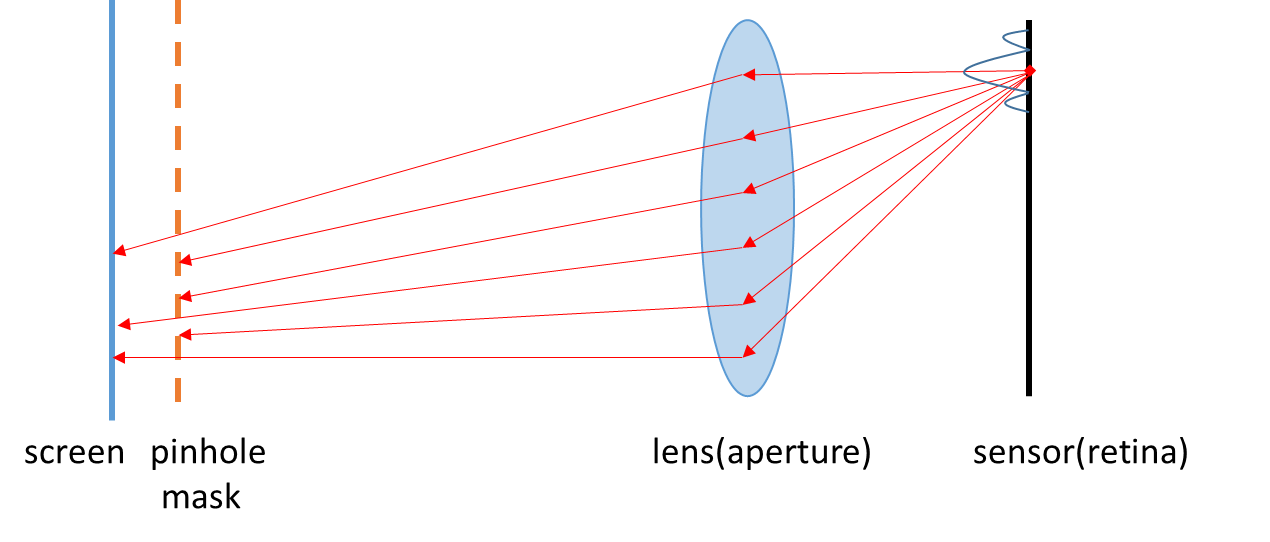
\includegraphics[width=4in]{chapters/chapter8/images/Diffract_Simulation.png}
  \caption{Wave Optics Simulation}
  \label{fig:ferrari}
\end{figure}


\lstset {language=C++}
\begin{lstlisting} [frame=single, caption=Pseudocode For Wave Optics Simulation]
int[][][] sensor = new int[sensor_size][sensor_size][3];
// Iterate over sensor pixels
for (int iy = 0; iy < sensor_size; iy++) {
  for (int ix = 0; ix < sensor_size; ix++) {
    int color[3] = {0, 0, 0};
    int hits = 0;
    // Iterate through random aperture points
    for (int i = 0; i < aperture_sample_time; i++) {
      sensor_pos = (ix, iy);
      aperture_pos = (aperture_samples[2*i], aperture_samples[2*i + 1]);
      type,color = getRayColor(sensor_pos, aperture_pos);
      if (value >= 0) {
        hits++;
	color[type] += value;
      }
    }
  }
  for (int x = 0; x < diffractMatrix.length; x++) {
    for (int y = 0; y < diffractMatrix.width; y++) {
       sensor[ix + x - diffractMatrix.length / 2][iy + y - diffractMatrix.width/2] += intensity[x][y] * color * 3 / hits;
    }
  }
}
\end{lstlisting}

\section{Results}

We compare the images produced by the physical experiment, ray optics simulation, and wave optics simulation. The parameters for all three cases are the same as those described earlier in the physical experiment section (380 millimeters focus distance, 250 millimeters display distance, 6 millimeters depth of pinhole mask, 6 millimeters diameter of human eye or f/8 stop, and 20 millimeters focal length). In addition, to see how well the ray and wave optics model account for diffraction, we examine the image quality of multiple pinhole sizes.

\subsection{Metrics}

The two metrics used to measure image quality are DRIM (dynamic range imagery) and RMSE (root mean square error).

\subsubsection{DRIM}

Aydin et. al 2008 describes DRIM as a metric that enables comparison of images with different dynamic ranges. The paper describes three measurements of image distortion: loss of visible contrast, amplification of invisible contrast, and reversal of visible contrast. We focus on loss of visible contrast, which occurs when contrast that was visible in the reference image becomes invisible in the test image. The algorithm in the paper applies a loss of visible contrast predictor and then a high-pass or low-pass filter. Here is what the distortion maps look like for the wave optics model for a 75 micrometer pinhole:

\begin{figure}[ht]
  \centering
  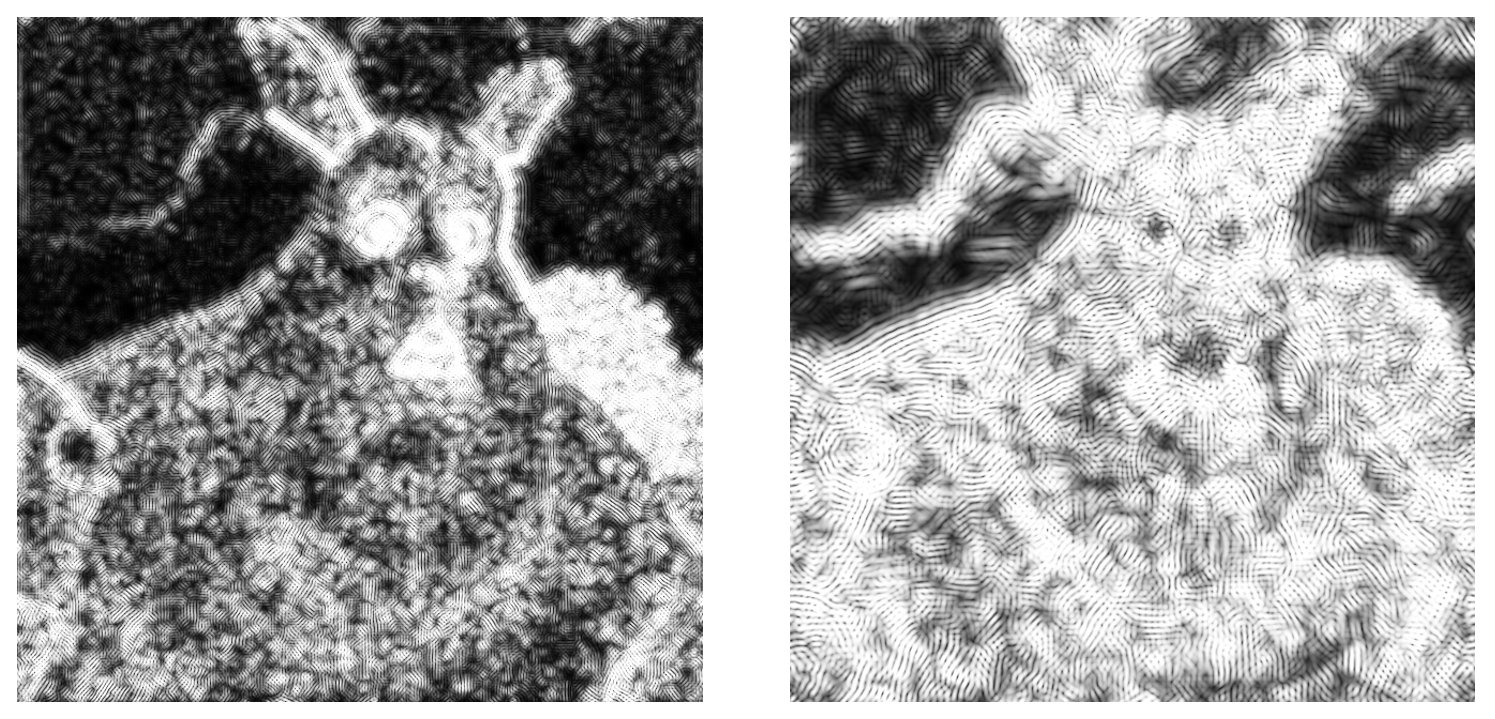
\includegraphics[width=3.5in]{chapters/chapter8/images/hp_lp_contrast_loss.png}
  \caption{Contrast Loss High Pass (left) and Contrast Loss Low Pass (right)}
  \label{fig:ferrari}
\end{figure}

The bright pixels represent areas of contrast loss. We compute the contrast loss as the pixel sum of the low-pass distortion image plus the pixel sum of the high-pass distortion image divided by two. 

\subsubsection{RMSE}

RMSE is a measurement used to measure how close the pixel values of the test image are to the reference image. $I_r$ in the equation below represents the RGB (red, green, and blue) intensities of the reference image, and $I_t$ represents the RGB intensities of the simulated image.

$$RMSE = \sqrt{ \sum_{y = 0}^{\textnormal{image length}} \sum_{x = 0}^{\textnormal{image width}} \sum_{c \in \{r,g,b\}} (I_r (x,y,c) - I_s(x,y,c))^2}$$

\subsection{Comparison of Ray and Wave Optics}

\begin{figure}[ht]
  \centering
  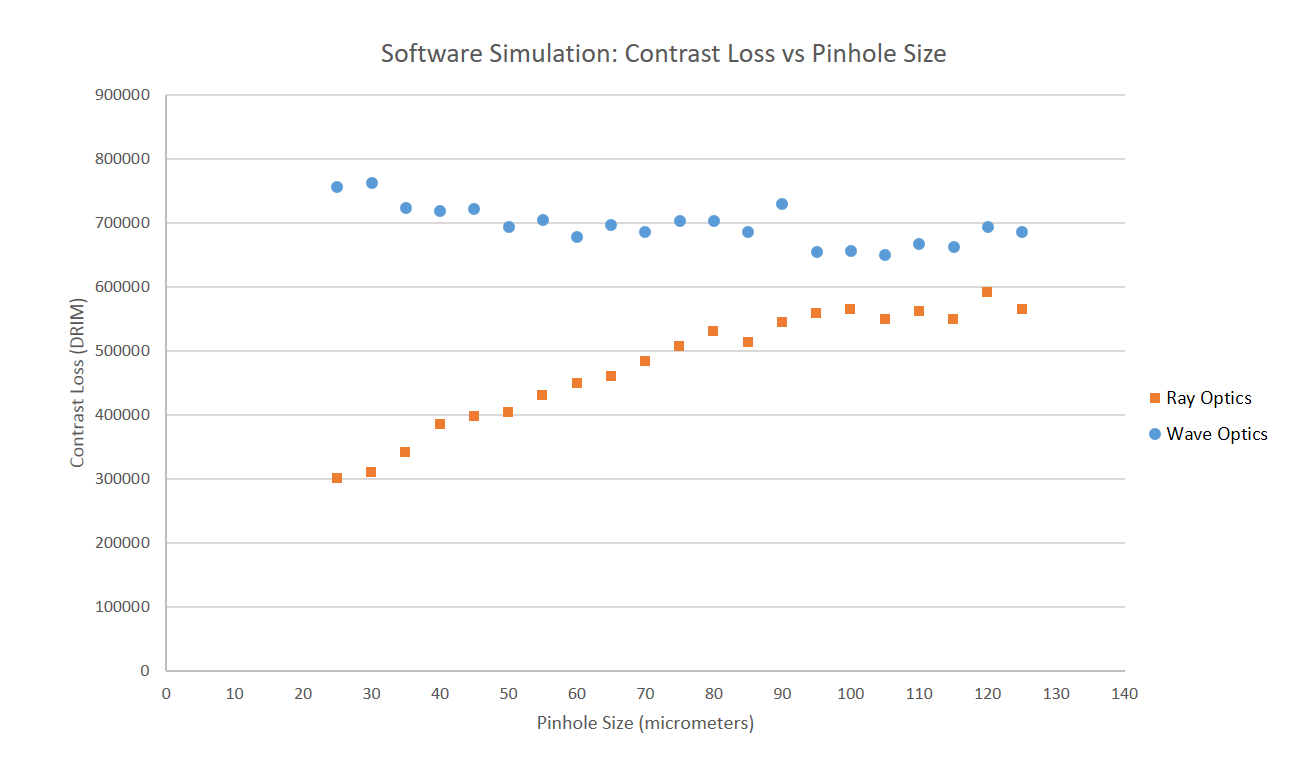
\includegraphics[width=7.0in]{chapters/chapter8/images/Contrast_Loss.png}
  \caption{DRIM Graph}
  \label{fig:ferrari}
\end{figure}

For the ray optics model, the larger the pinhole size, the worse the contrast. The pinhole size that gives the least loss of contrast is 25 micrometers. A pinhole of size 120 micrometers (contrast loss of about 600,000) generates twice the amount of contrast loss as a pinhole of size 25 micrometers (contrast loss of about 300,000). These results are expected because smaller pinholes focus light, which leads to sharper image contrast. For the combined ray and wave optics model, the contrast loss from different-sized pinholes is roughly the same (between 640,000 and 770,000). We find that the benefits of a small aperture in filtering light are counterbalanced by the larger diffraction pattern that is created. The smallest pinhole sizes create the largest diffraction patterns and therefore have the most severe contrast loss. From 25 micrometers to 105 micrometers, there is a weak trend of improving contrast due to the effects of diffraction outweighing the sharper focus of light through the pinhole. From 105 micrometers to 125 micrometers, there is a weak trend of declining contrast because at that point, the diffraction effects are very minor, and the larger pinhole sizes reduce the depth of field and do not focus the light source well. A pinhole size of 105 microns generates an image with the most contrast.

\begin{figure}[ht]
  \centering
  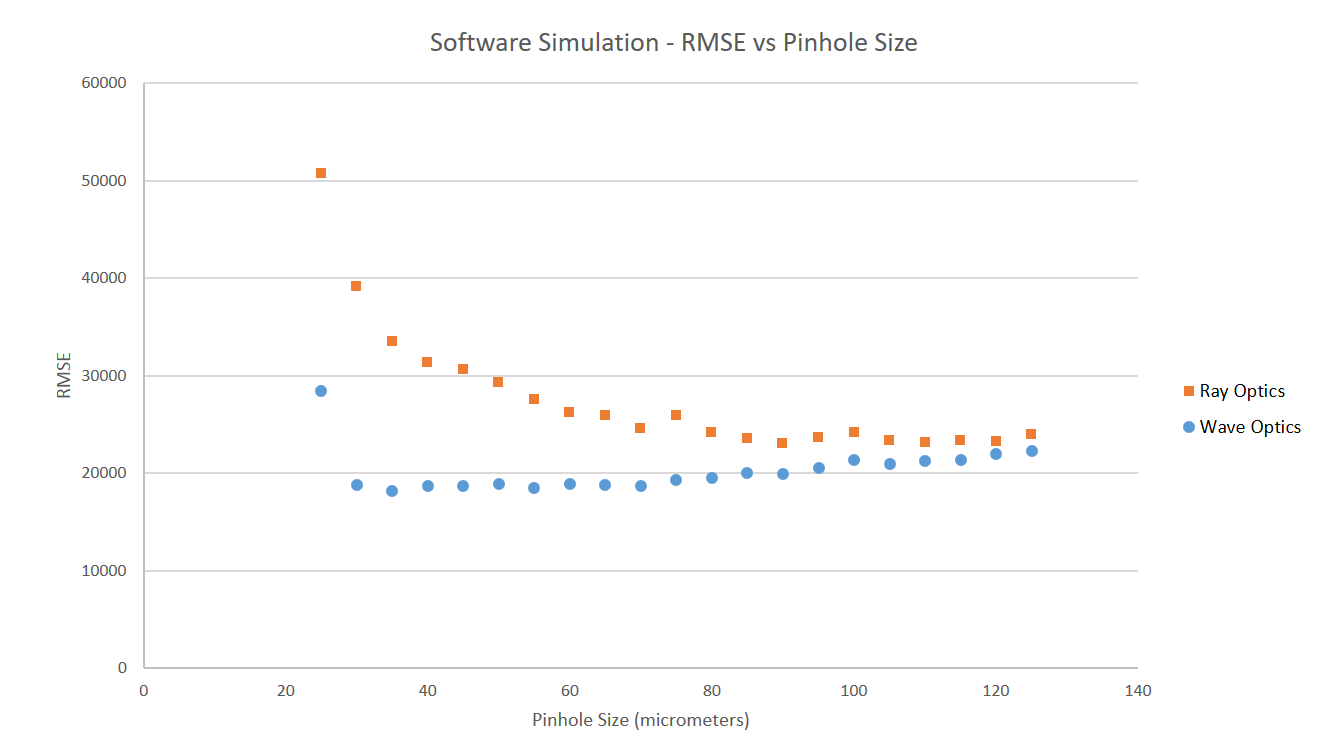
\includegraphics[width=7.0in]{chapters/chapter8/images/RMSE.png}
  \caption{RMSE Graph}
  \label{fig:ferrari}
\end{figure}

For the RMSE metric, the wave optics model features improvement over the ray optics model, despite the fact that the wave optics model produces a blurred version of the ray optics model. For both models, small pinhole sizes create an amplification of contrast, which leads to a larger RMSE. In addition, since small pinhole sizes allow significantly fewer light rays to reach the screen, there is a greater possibility of having too many rays of one color (red, green, or blue) and getting a noisy image (see figure 14 below). Because blurring reduces this amplification of contrast, larger pinhole sizes have smaller RMSE values for the ray optics model, and the wave optics model consistently produces images with smaller RMSE than the ray optics model. The wave optics model shows a trend of increasing RMSE for pinhole sizes 75 micrometers and above, because at that point, there is no more amplification of contrast, and blurring only causes the modeled image to deviate further from the clean image. Although a smaller RMSE is expected to indicate a image with pixel values close to the original image, it actually has a high chance of indicating more blur. Therefore, RMSE is a poor indicator of contrast and mediocre indicator of image quality. 

\begin{figure}[ht]
  \centering
  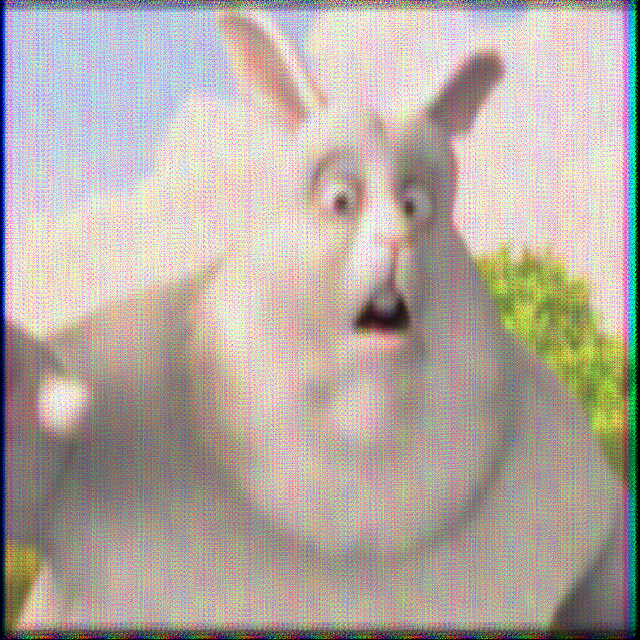
\includegraphics[width=2in]{chapters/chapter8/images/simulationResult_25.png}
  \caption{Ray Optics Simulation for 25 micrometer pinhole mask}
  \label{fig:ferrari}
\end{figure}

\subsection{Comparison of Physical Experiment and Software Simulation}

\begin{figure}[ht]
  \centering
  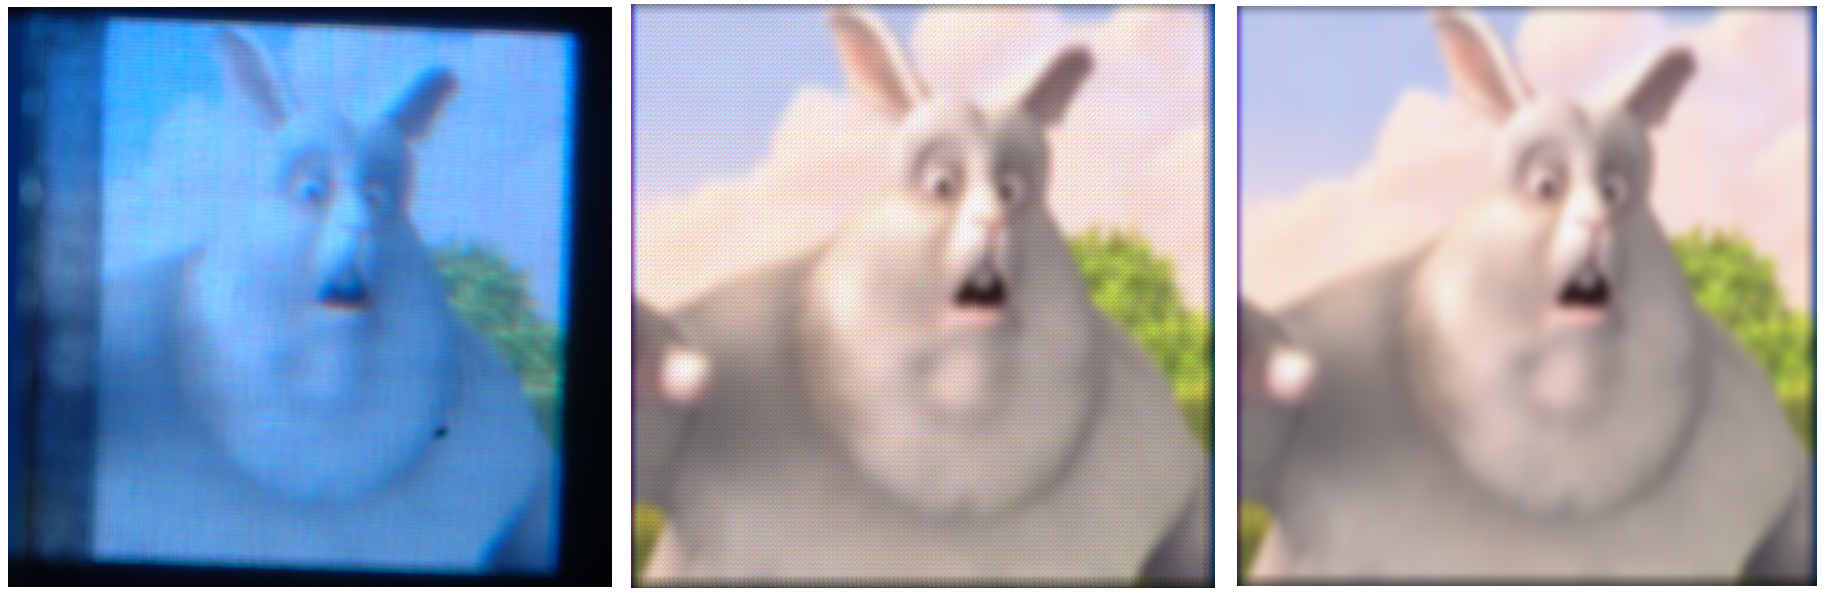
\includegraphics[width=5in]{chapters/chapter8/images/Comparison.png}
  \caption{Left: Physical Experiment, Center: Ray Optics Simulation, Right: Wave Optics Simulation}
  \label{fig:ferrari}
\end{figure}


We compare the images produced by the physical experiment, ray optics simulation, and wave optics simulation for a 75 micrometer pinhole. The wave optics simulation is slightly more blurred than the ray optics simulation, which is expected. Interestingly enough, the physical simulation generates the clearest image, but the exposure had to be inflated in order for the physical simulation to work. If one looks closely at the physical experiment image and the ray simulation image, one will find that a grid pattern is visible on both the physical experiment image and ray optics image, but is removed from the wave optics image due to diffractional blur. This shows that perhaps the wave optics simulation created a blur pattern that was too large for the 75 micrometer pinhole. 

\section{Conclusion and Future Work}

The physical experiment and the software simulation give mixed results. The prefiltering algorithm combined with the pinhole mask display yields a significant improvement to the defocused image. The ray optics model yields an image that has slightly less contrast than the one in the physical experiment and recommends using the smallest pinhole size to achieve the best contrast as long as RMSE is not too high. The wave optics model gives even more blurred images than the ray optics model and recommends using a larger pinhole size of approximately 105 micrometers to achieve an image with the best constrast. There exists a slight contrast gap between the physical experiment and software simulations that needs to be resolved.

In the future, we will try to find more ways to improve on the ray and wave optics model to look more like the physical experiment. One area to expand on in the wave optics model is to consider the light ray as a Gaussian beam rather than a point source. In addition, we would like to test the ray and wave optics models for astigmatism, another form of lower order aberrations, and higher order aberrations like coma and trefoil. We would also be interested in running physical experiments with pinhole masks for different sizes to confirm the results of the ray and wave optics models. 

\chapter{Comparison of Different Algorithms}

% Do a good job of explain PSNR via this paper: https://en.wikipedia.org/wiki/Peak_signal-to-noise_ratio

We compare the performance of the different algorithms used throughout this report. We also test the performance of the forward method and backward method on different pinhole sizes (3x3 pinhole vs 5x5 pinhole). Potential advantages of the 3x3 pinhole include improved resolution. However, the 3x3 pinhole filters out less light than the 5x5 pinhole, which can lead to more blurring.  

\begin{figure}
    \centering
    \textbf{3x3 Forward Algorithm}\par\medskip
    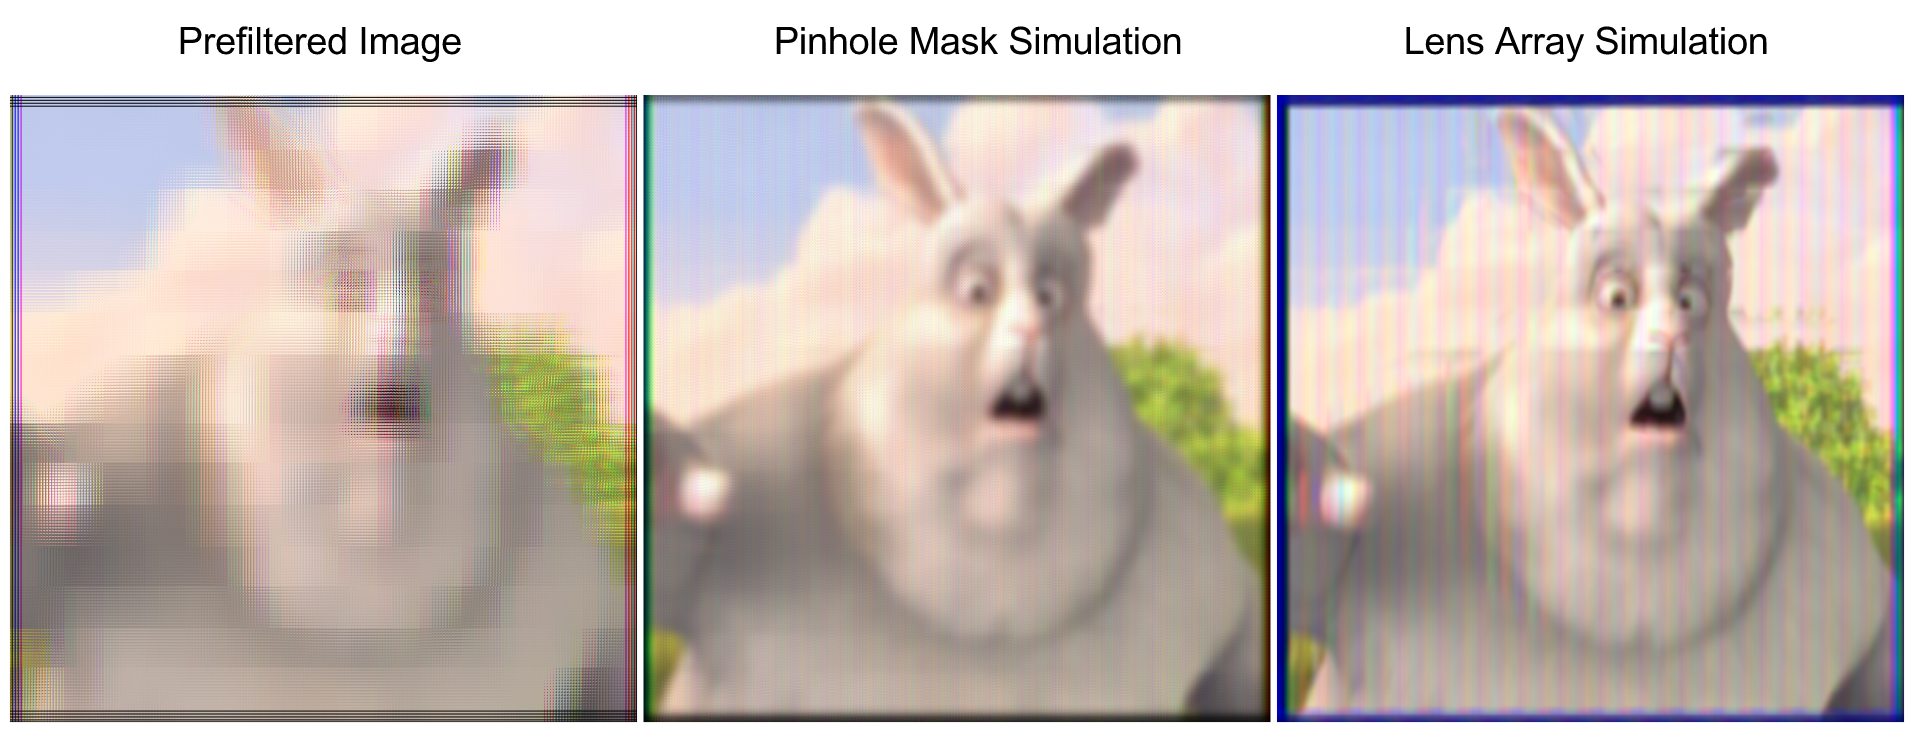
\includegraphics[width=\columnwidth]{chapters/chapter9/images/3x3_forward.png}
\end{figure}

\begin{figure}
    \centering
    \textbf{5x5 Forward Algorithm}\par\medskip
    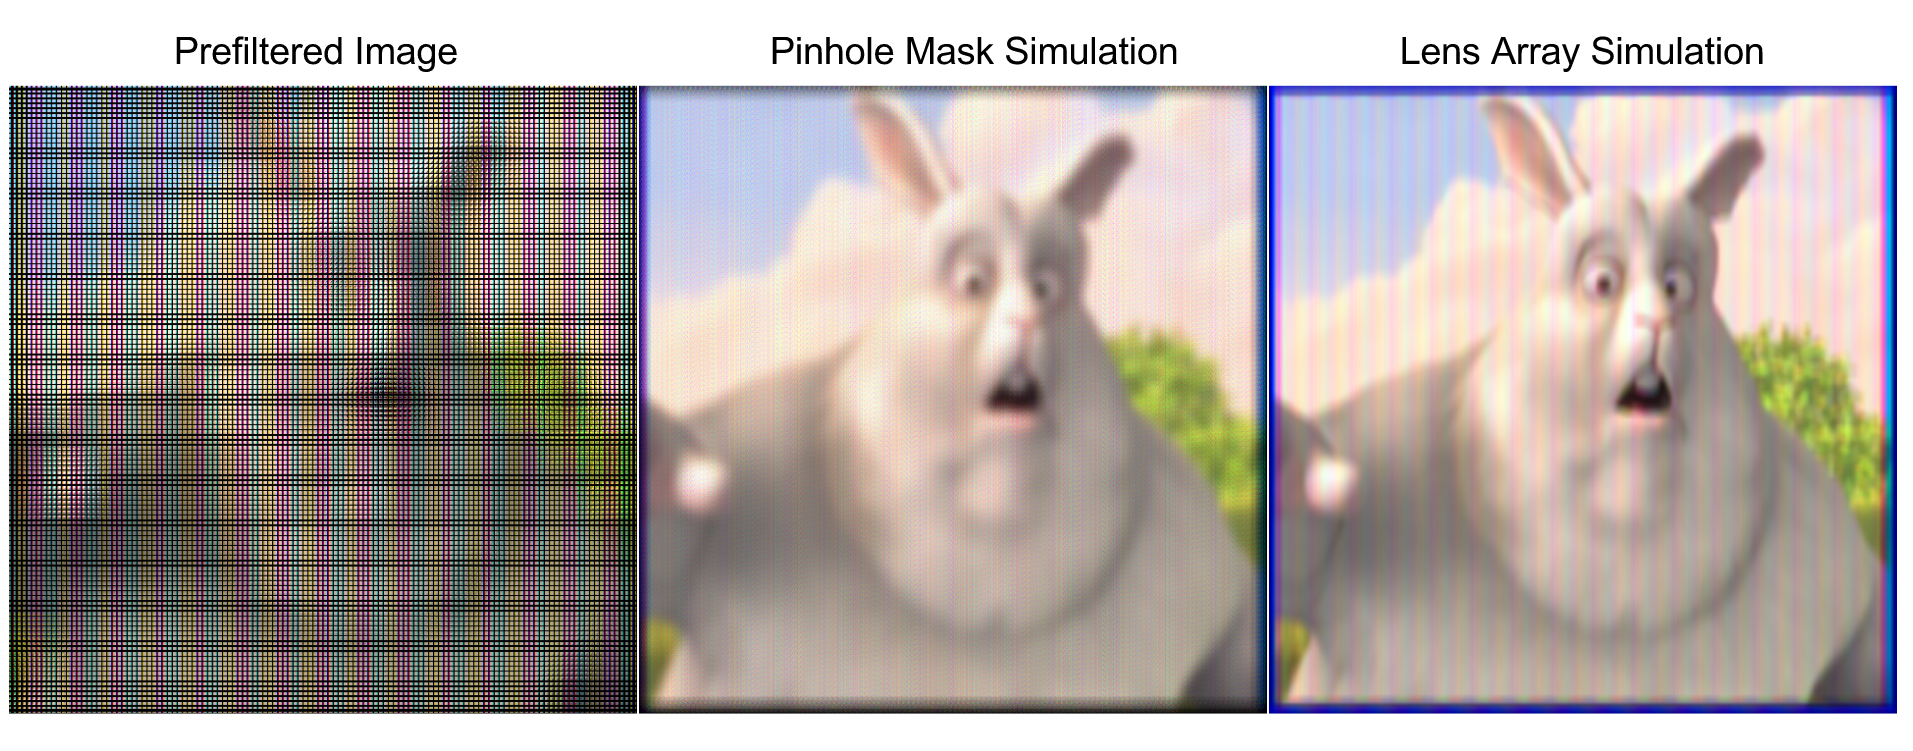
\includegraphics[width=\columnwidth]{chapters/chapter9/images/5x5_forward.png}
\end{figure}

\begin{figure}
    \centering
    \textbf{3x3 Backward Algorithm}\par\medskip
    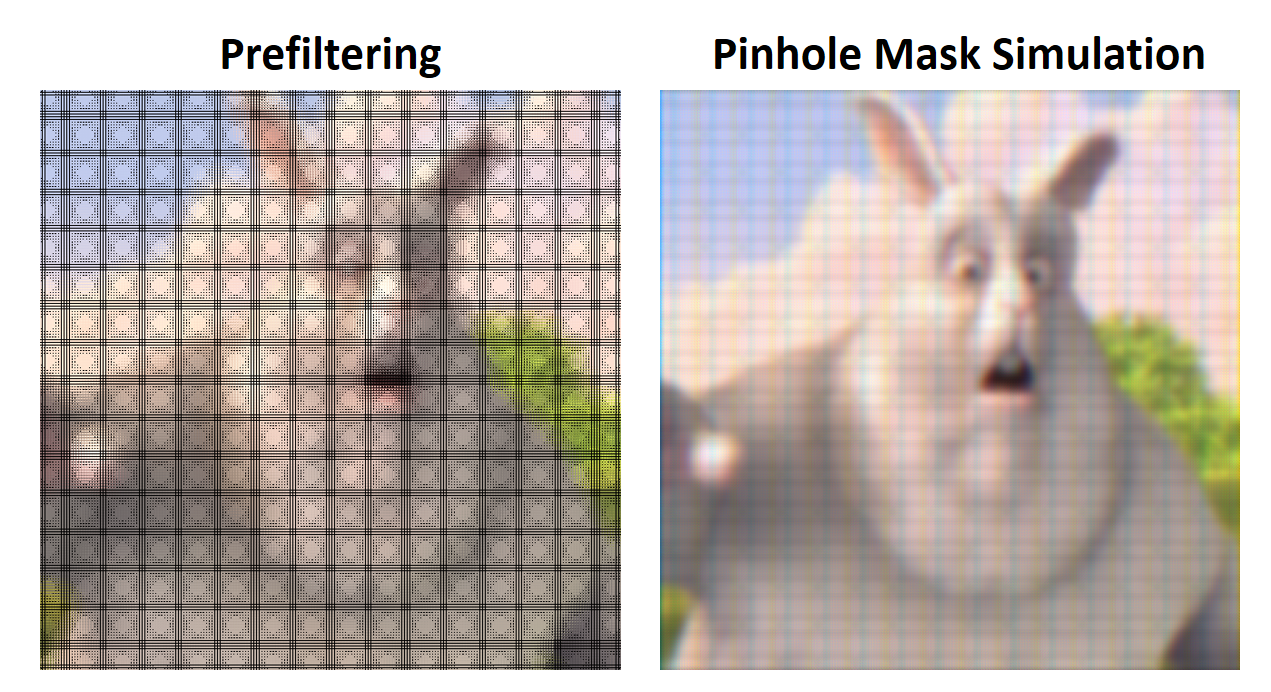
\includegraphics[width=\columnwidth]{chapters/chapter9/images/3x3_backward.png}
\end{figure}

\begin{figure}
    \centering
    \textbf{5x5 Backward Algorithm}\par\medskip
    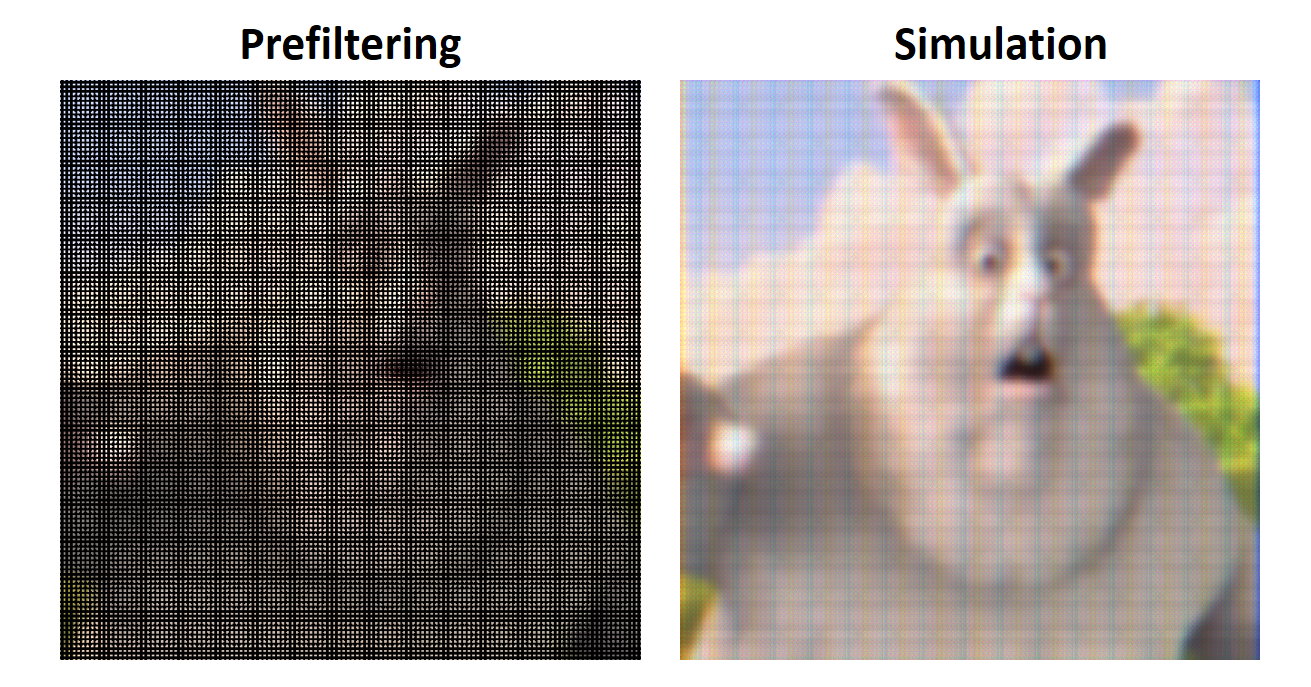
\includegraphics[width=\columnwidth]{chapters/chapter9/images/5x5_backward.png}
\end{figure}

\begin{figure}
    \centering
    \textbf{Huang's Algorithm at One Angle}\par\medskip
    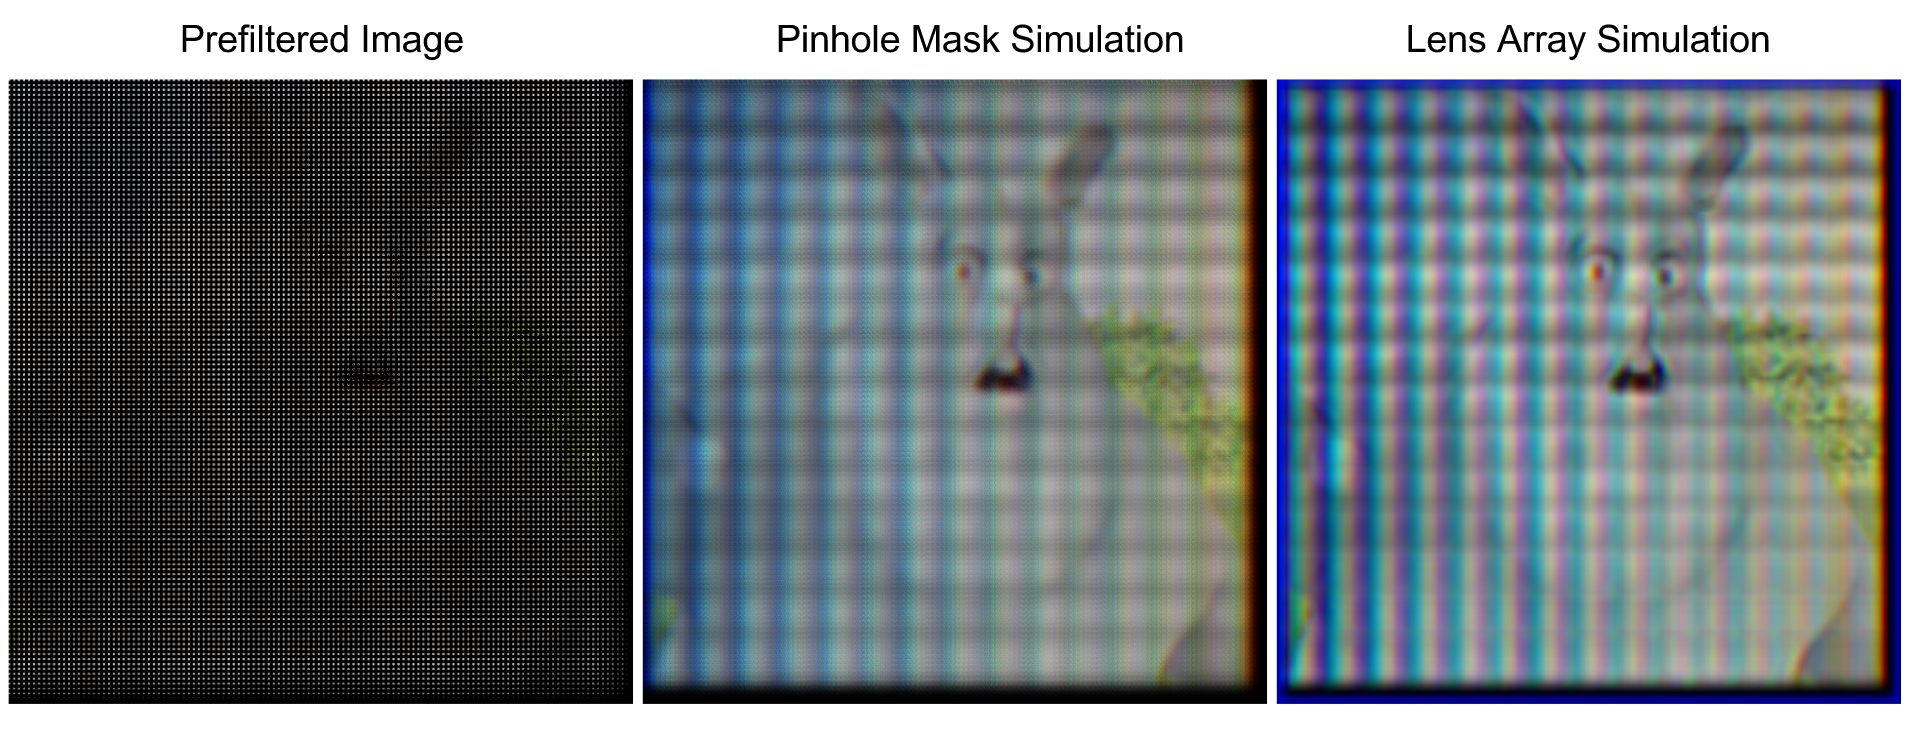
\includegraphics[width=\columnwidth]{chapters/chapter9/images/Huang_1_angle.png}
\end{figure}

\begin{figure}
    \centering
    \textbf{Huang's Algorithm at All Angles}\par\medskip
    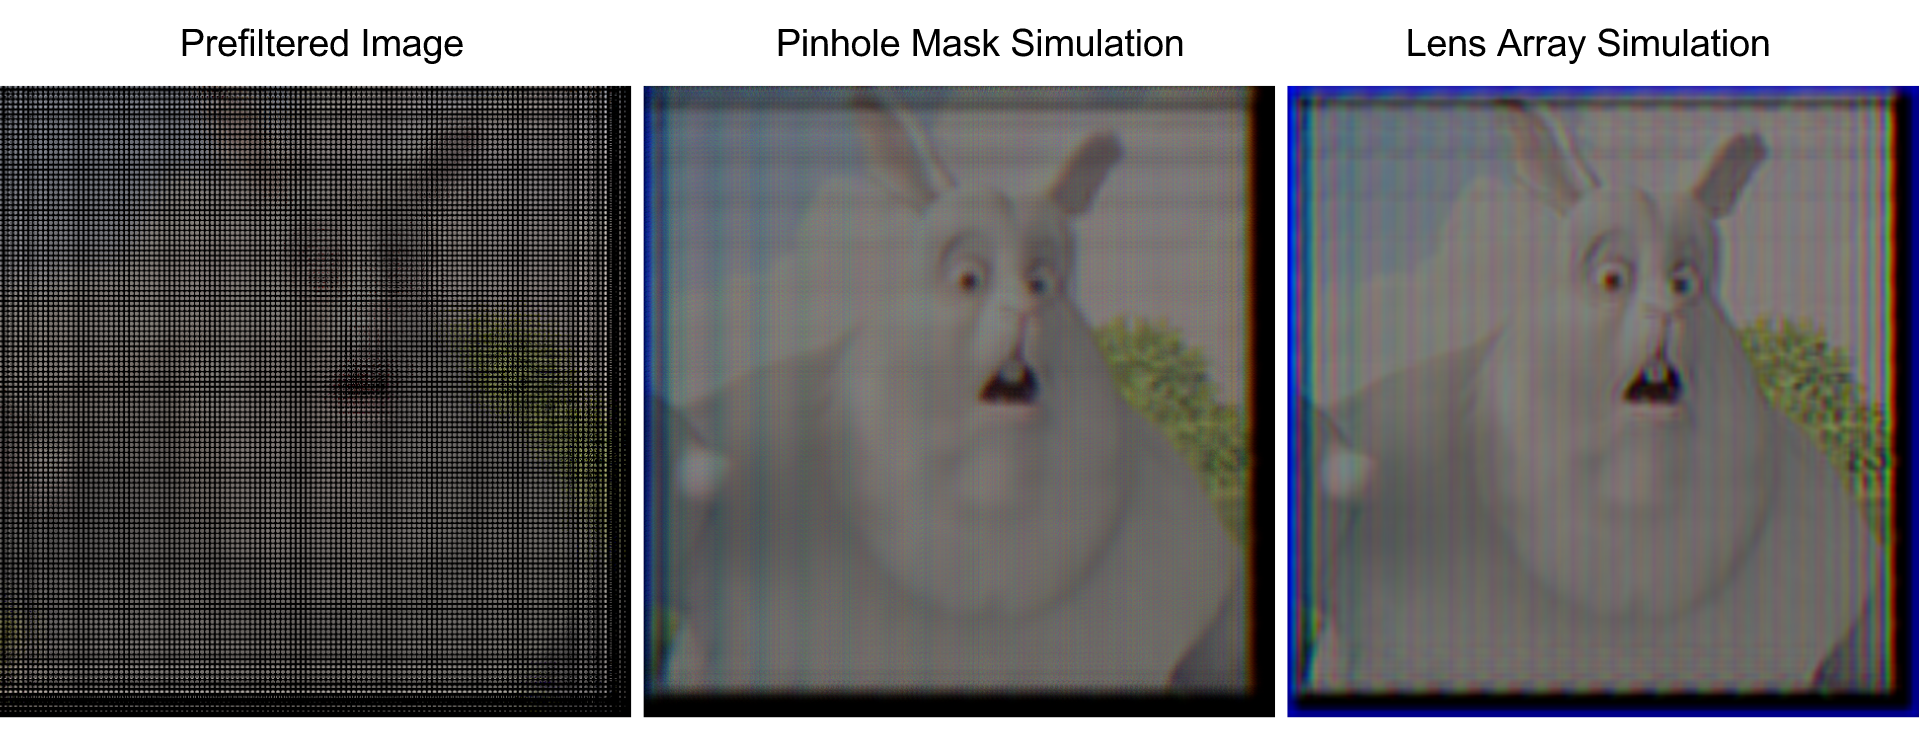
\includegraphics[width=6in]{chapters/chapter9/images/Huang_all_angle.png}
\end{figure}

\begin{figure}
    \centering
    \textbf{RMSE}\par\medskip
    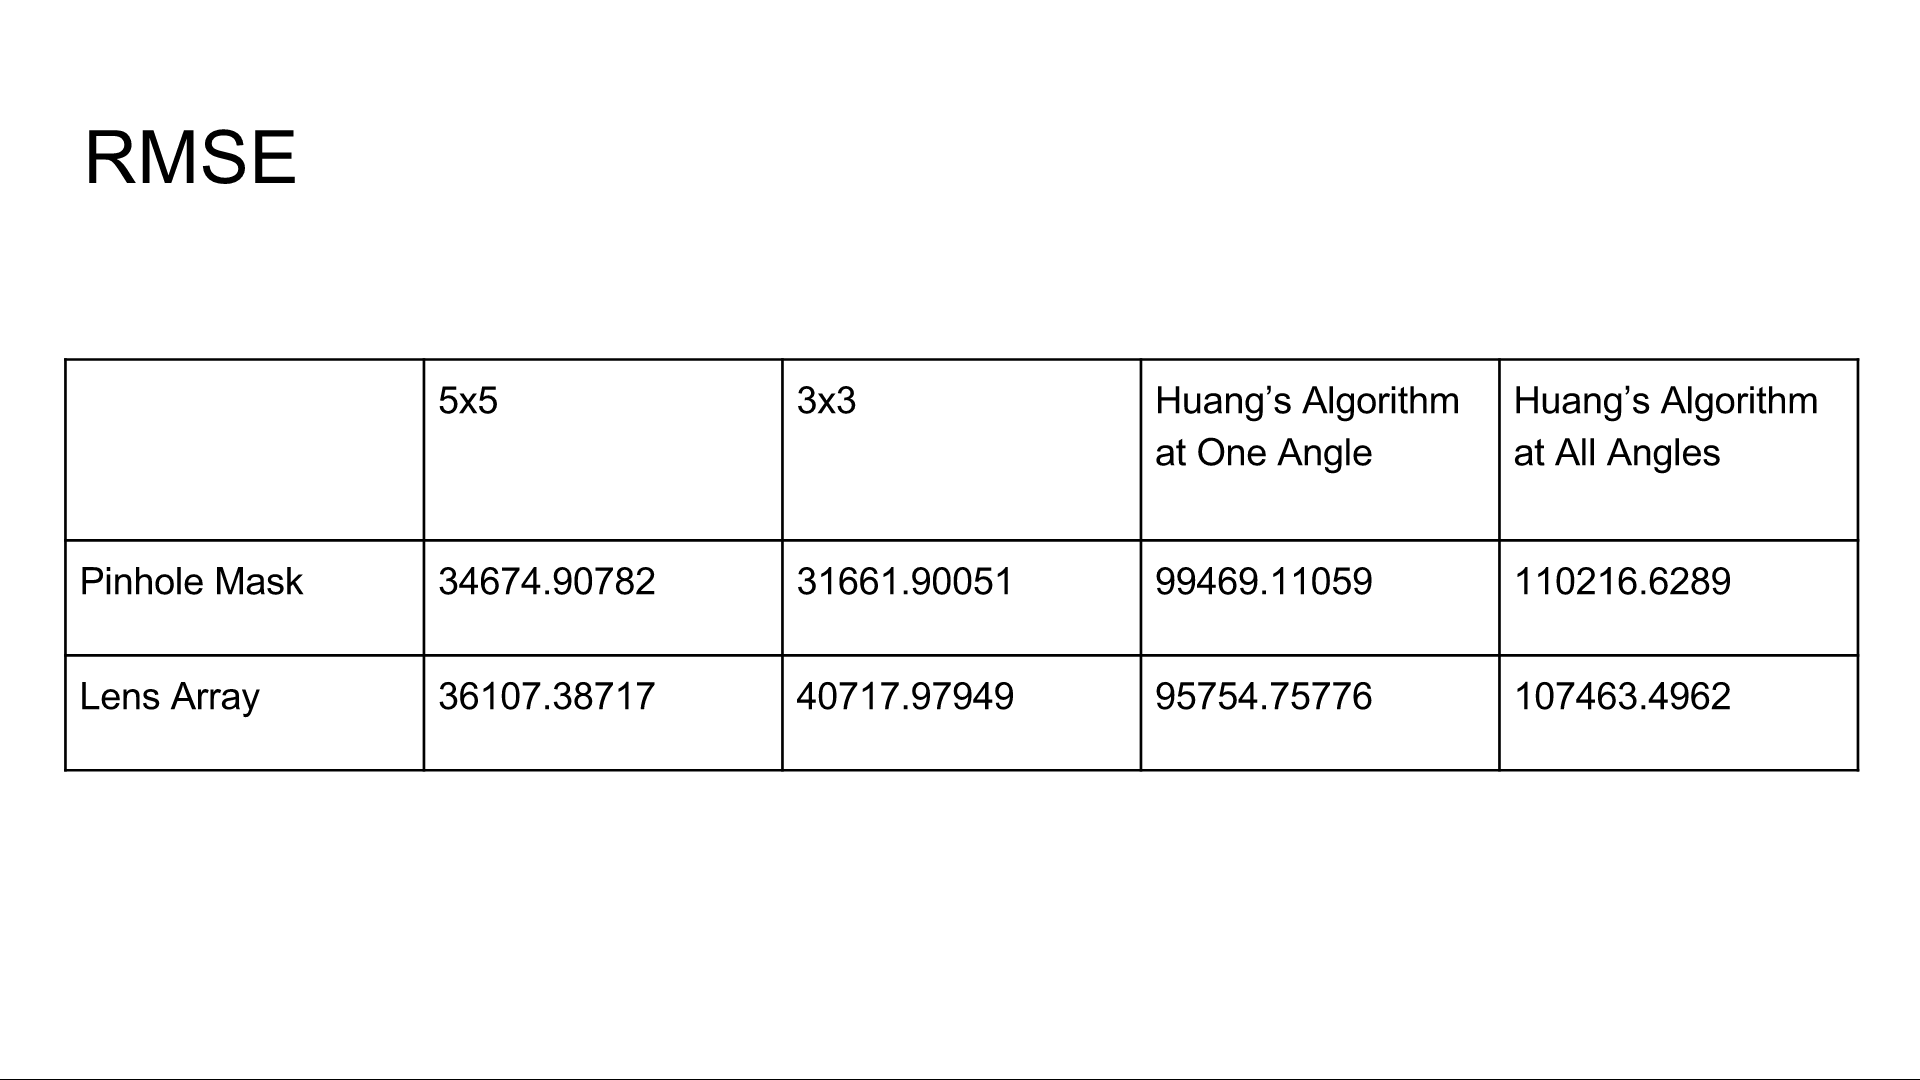
\includegraphics[width=6in]{chapters/chapter9/images/RMSE.png}
\end{figure}

\begin{figure}
    \centering
    \textbf{PSNR (Peak Signal to Noise Ratio)}\par\medskip
    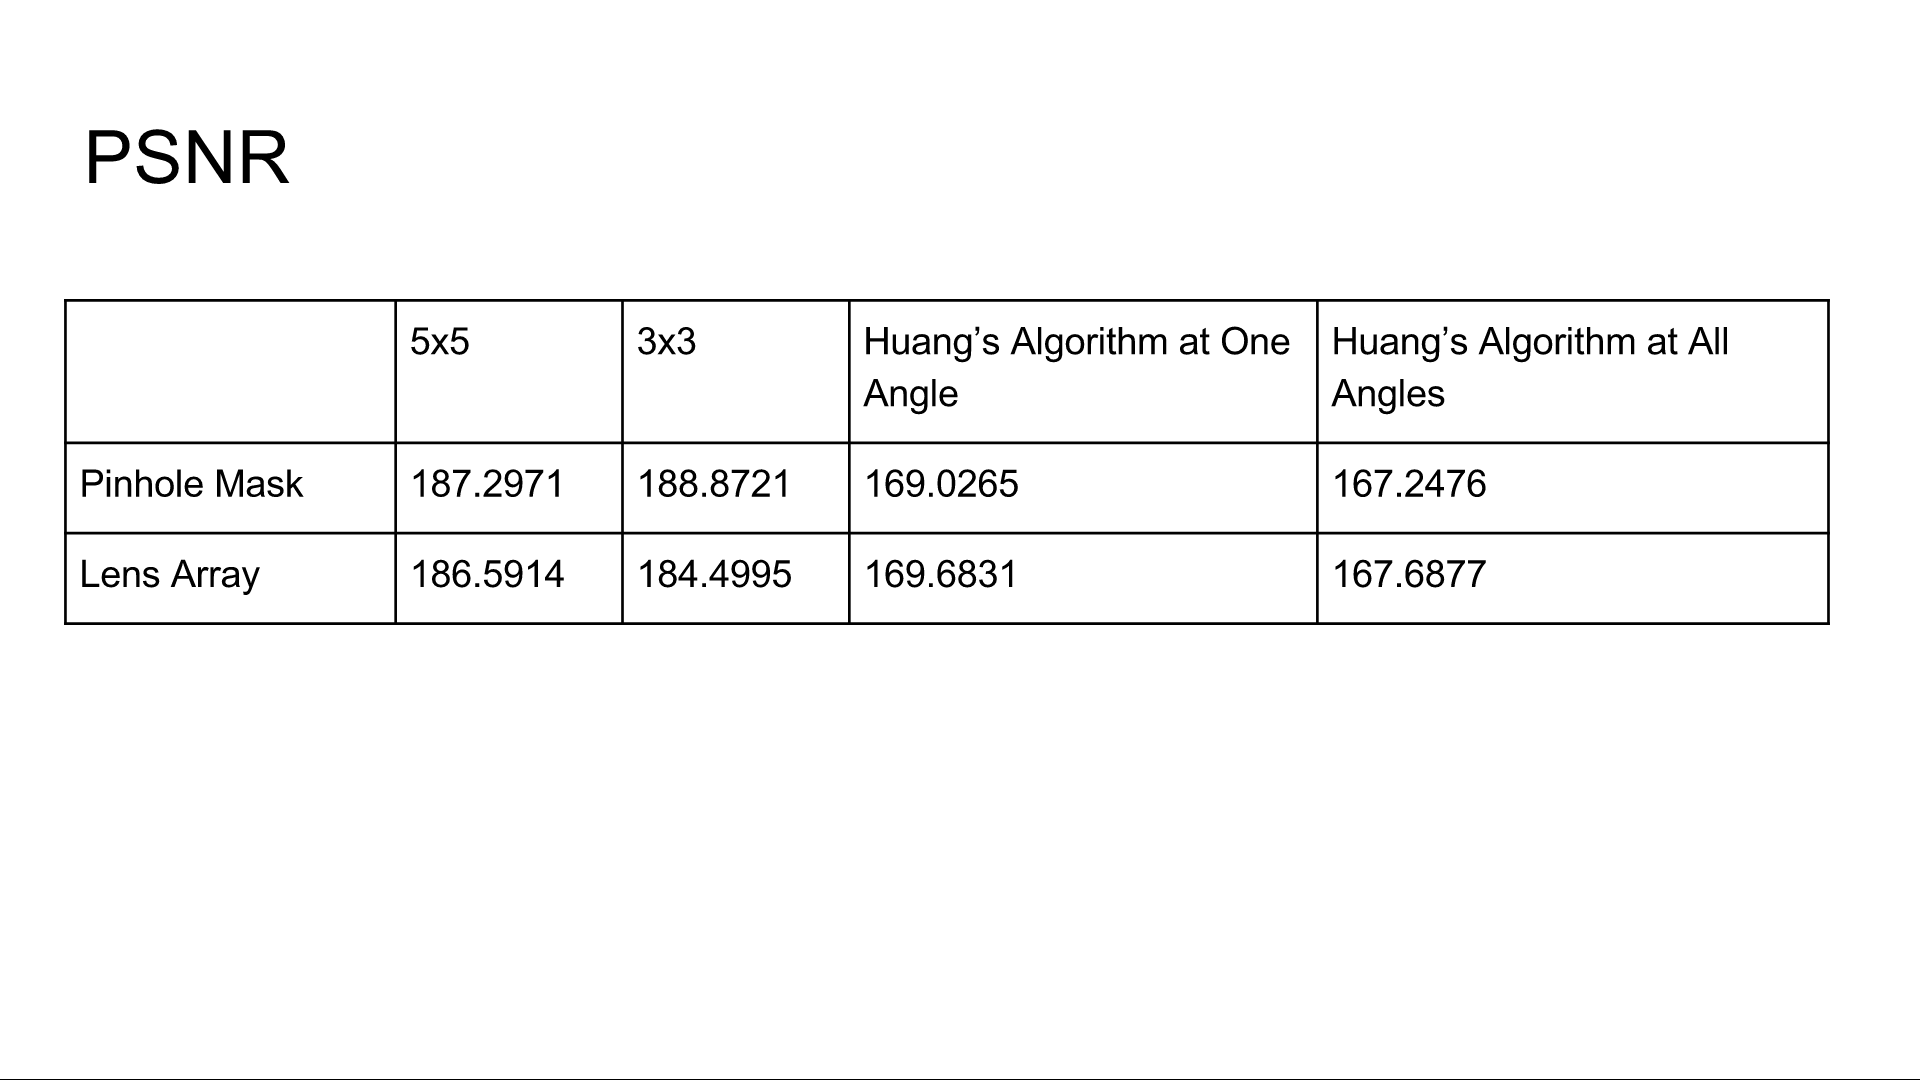
\includegraphics[width=6in]{chapters/chapter9/images/PSNR.png}
\end{figure}

\begin{figure}
    \centering
    \textbf{Contrast Loss}\par\medskip
    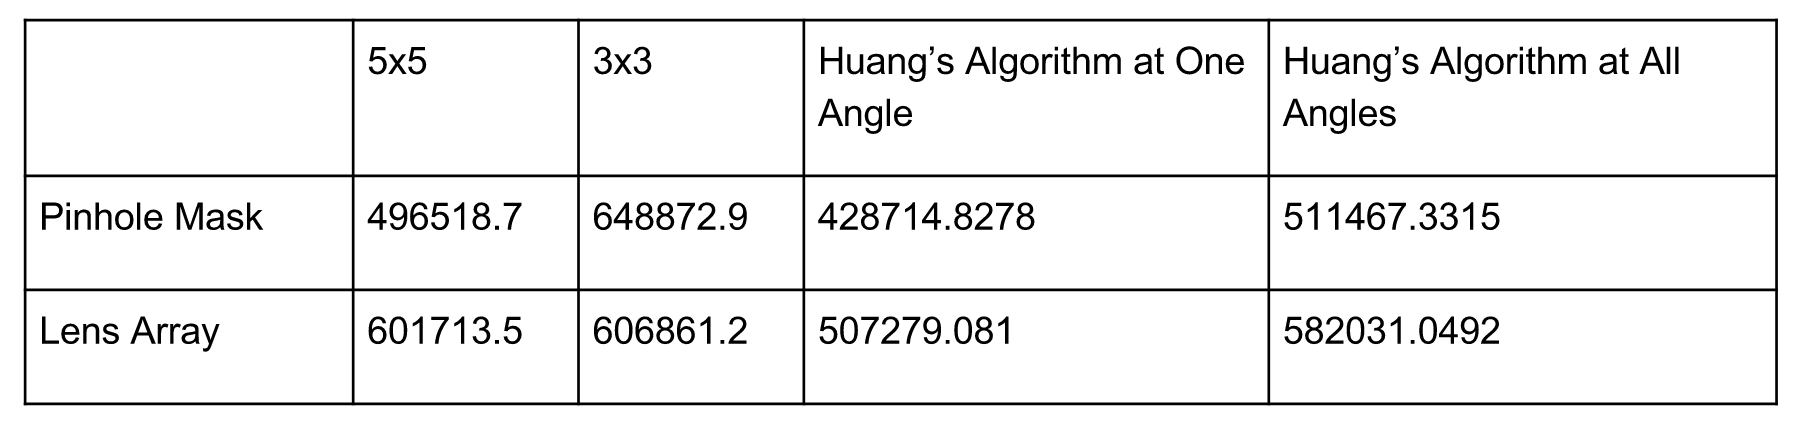
\includegraphics[width=\columnwidth]{chapters/chapter9/images/Contrast_Loss.png}
\end{figure}


\chapter{Conclusion}

In conclusion, the results of the physical experiment and software simulation show that the vision correcting display drastically improves the quality of vision for people with eye aberrations. As the number of people with vision problems increases and the time people spend on digital screens increases, new methods for correcting aberrations will become more and more necessary. The backward method proposed runs faster than the comprehensive version of Huang's algorithm and produces clearer images than the forward method depending on the light field display and angular resolution. The forward method and simulation algorithm work well regardless of the pixel arrangement of the device. The wave optics simulation takes into account diffraction through the pinhole mask and has many applications in optical physics. 

In the future, vision correcting displays will present a viable alternative to eyeglasses, contact lenses, and refractive eye surgery for people who want to view screens clearly. With the rapid increase in computing power, the algorithms will be able to run in real-time. Eye tracking software will be able to determine the parameters like distance to the eye. The next time a person watches TV or reads from a phone, he or she will not even remember his or her eye problems.

% Make the last sentence sound better

\printbibliography

\end{document}